\documentclass{article}
\usepackage[utf8]{inputenc}
\usepackage{pifont}
\usepackage{fullpage}
\usepackage{graphicx}
\usepackage{subcaption}
\usepackage{color}
\usepackage{todonotes}
\usepackage{amsmath}
\usepackage{amssymb}
\usepackage[final]{microtype}
\usepackage[backend=biber, sorting=none]{biblatex}
\newcommand{\cmark}{\ding{51}}%
\newcommand{\xmark}{\ding{55}}%

\newcommand{\SMC}{{\tt smcsmc }}

\title{Evidence for Directional Migration to Africa and Population Structure in the Paleolithic}
\title{Genomic Evidence for Prehistoric Migrations to Africa and Population Structure in the Paleolithic}
\author{}
\date{}

\addbibresource{migration-paper.bib}

\begin{document}

%
%\paragraph{Outline}
%\begin{enumerate}
%    \item Introduction
%    \item Methods
%    \item Current Results 
%    \begin{enumerate}
%        \item Effective population sizes from SMC2 and MSMC, which finds differences in the earlier periods. This is similar to what was seen in PSMC.
%        \item To investigate this, we simulate things like PSMC, and find that we also can recover the incorrectly high population size. (What could be causing this high population size?)
%        \item Migration rate inference shows a peak of migration after this time period, acting as a possible explanation for the inflated population size. This trend breaks down mostly by language group (which are also validated evolutionary phyla). 
%        \item Concerns about the phasing methodology made us validate this in HGDP. Language groups main trends line up well with results from SGPD.
%        \item Migration initialisation is important, talk about how different starting values can give different results. Include a brief supplemental section about seeding away from symmetric migration.
%        \item We can isolate the segments with a migration event in their history by using SMC2's estimated ARG. We can use these segments to look at the relationship between these individuals and all of the others in SGDP. We find that our statistics in our segments are higher, meaning that the segments are indeed more Eurasian.
%        \item Briefly talk about expectation of segment length, and how ours is consistent with a very large migration in that period, though we think this is unlikely, it does line up with the later evidence from the simulations. Caveats: not a single pulse (which makes it less than ideal, ideally would integrate similar to earlier paper (but this is very difficult to do analytically)), estimates not accurate with large values, selection almost certainly a factor.
%        \item We simulate to find situations consistent with what we see, and find that we can recover basically the exact same thing with very large migration pulses. This is unrealistic, and means that we have some bias, at some level dependant upon the age of the migration, which is affecting inference. A large migration is consistent with the migration segments analysis, but is unlikely.
%        \item {\textbf We use the segments we have to estimate relationships between the segments and a panel of ancient individuals, to try to get more clarity on the donating population. Ideally some estimate of consistency among populations, and pull in the average $D$ statistic calculation. Not sure what the results will be here.}
%        \item We look at the relationship between the segments and Neanderthals, which are known to have contributed to OoA groups around this time period. Talk about the SMC2 analysis with Vindija, and Kay's analysis with the $D$ statistics (which I will have to rerun).
%        \item  {\textbf We also use these $D$ statistics to estimate a demographic model with ADMIXTOOLS, and show the resulting best-fit graph. Not sure what the results will be here.}
%    \end{enumerate}
%    \item Discussion
%\end{enumerate}
%
%
%Things to (possibly) do.
%    
%\begin{enumerate}
%    \item \xmark Run MSMC alongside the actual inference, get the MSMC $N_e$ estimates on the same samples, overlay the plots. Have a figure which directly compares them on one particular case, then a supplemental that will have all of them with this overlay. Will probably want to include the x-coal rate somewhere in here. Put it on the migration plots probably.
%    \item \cmark PSMC simulations have to be re-run with the correct migration parameter. (These are actually only single haploid inference, so they're fine. The simulations in general have to be rerun, but these ones are okay as is.)
%    \item \cmark Simulations have to be run with the same magnitudes...? Did I do these already? Yes, I have all the magnitudes that I want, and I've run more midpoints with the different initiationalisation values for migration. 
%    \item (Long) Run all groups in Africa with the correct migration initiation. Ideally against a few different groups (French, Han, Papuan, something else)
%    \item (Long) Replicate the SGDP runs with the HGDP.
%    \item After the whole thing is done, do the $D$ statistics with all versus segments (ideally for all of the "ascertainment" schemes), and reproduce the plots from before.
%    \item The segment length estimation has to be redone, but there isn't all that much to do here.
%    \item Maybe redo a Vindija run, maybe not. 
%    \item Kay's Neanderthal analysis has to be redone with the new segments. Hopefully this should be straightforward, as I'll just have a script that reruns his particular statistics. This will be a table, like the one in his Nddth paper, with the individdual statistics picked out. The rest can go in a Supplemental section.
%    \item Admixturegraph if its possible.
%\end{enumerate}
%
%
%List of figures / tables:
%
%\paragraph{Figures}
%
%\begin{enumerate}
%    \item a) SMC2 versus MSMC population size inference for a case or two b) PSMC simulation that shows the same thing.
%    \item a) Migration inference by language phyla (possibly superimposed all on top of each other), along with HGDP validation. b) Initialisation conditions. c) Segment lengths (by replicate, and HGDP/SGDP)
%    
%\end{enumerate}
%
%\paragraph{Supplementary Figures / Sections}
%
%\begin{enumerate}
%    \item All of the SMC2 versus MSMC $N_e$ inference
%    \item All of the PSMC simulations.
%    \item Migration rate inference in SGDP and HGDP (with error bars)
%    \item Kay's statistics, and maybe add in an SMC2 run with the vindija. This is a low priority.
%    \item Probably a section for the "rest" of the D statistics, because I probably won't be able to use all of them. Potentially this can be a file though, instead of a table. The table doesn't really tell you very much. 
%\end{enumerate}
%
\newpage

Things remaining (that require computation):

\begin{enumerate}
	\item Vindija SMC2 run with lower migration (2 days?)
	\item Shum laka run (ancient African) (2 days) WGS at reich lab
	\item MSMC on HGDP (2-3 but maybe 4-5 days)
	\item Finish migration simulations, if they aren't already done (2 days)
\end{enumerate}

Total approx a week, not including qpgraph.

Things remaining (that don't):

\begin{enumerate}
	\item Demography figure
	\item Admixturegraph? I really don't see this happening.
	\item Write supplemental section describing full SGDP analysis
	\item Similarly with HGDP
	\item Supplemental section on simulation procedure
\end{enumerate}

Questions for Gerton / think about:

\begin{itemize}
	\item What to do with $D$ statistics? Maybe could combine all papuan statistics and all modern Eurasian statistics and that that they're less? Ideally I could jusst rerun this with different groups, but I could also take the average across the populations.
	\item I could also 

\end{itemize}

\newpage

\maketitle

\begin{abstract}
	African population structure prior to the expansion of agricultural and pastoral groups in the Holocene is largely unknown. Recently, several studies have attributed previously unexplained patterns in genetic variation to anciently diverged, unsampled populations. Using a novel particle filter method to estimate effective population size and directional migration rates over time in the Simons Genome Diversity Panel and the Human Genome Diversity Project, we find that over the last 100ky, approximately 50-60\% of the ancestors of modern day Niger-Kordofanian and Nilo-Saharan populations were replaced by a migration from a group more related to Han Chinese and French than to Papuans. South and Central African hunter gatherer populations show lower levels of migration, though both groups have a consistent peak of inferred migration between 50 and 70kya. We show that this migration has inflated previous estimates of population size and that by accounting for it, we recover a more recent split-time between African and non-African populations. This analysis consolidates suggestive evidence from many previous studies in support of a large-scale contribution to the ancestors of Western Africans from a ghost population related to the Out of Africa migrants.
\end{abstract}

\section{Introduction}

The early population structure of anatomically modern humans (AMHs) in Africa and their eventual migration into the Eurasian continent have shaped global patterns of genetic variation \cite{Pagani2016, Nielsen2017a}. However, little is known about population structure within Africa prior to the expansion of agriculturalists and pastoral groups \cite{Busby2016, Patin2017}. Recent evidence from the handful of successfully sequenced ancient African genomes hint at large-scale population movements and admixture from multiple highly divergent, extinct populations, with complex affinities to current groups \cite{Skoglund2018, Lipson2019, GallegoLlorente2015a}. The majority of structure in the continent is derived from events in the Holocene, including the spread of Bantu languages from Western Central Africa both East and South, as well as admixture from pastoralists its in the Near East and Western Eurasia \cite{Busby2016}. Eastern Africans are the most closely related group to the ancestral Out of Africa migrants, though they show particularly high levels of ancestry related to neolithic populations from Iran and the Levant consistent with multiple waves of back-migration in the Holocene \cite{Skoglund2017}.  Evidence for recent admixture from Eurasian sources is well established, however the lack of ancient African DNA from the Pleistocene has confounded efforts to uncover interactions between the earliest inhabitants of the continent. While the migration event associated with establishing current global population structure has been confidently dated between 60-80kya, Central and South African hunter gatherers such as the Mbuti and KhoeSan (without implying linguistic unity, defined as southern African hunter gatherers who speak non-Bantu languages which include a click consonant) may have diverged from other groups 200-250 thousand years ago (kya) \cite{Lipson2019, Schlebusch2017}. In the intervening millennia, fossils identified as AMH have been found in China about 80-120kya, Sumatra about 63-73kya, and artifacts from Australia 65kya \cite{Clarkson2017, Liu2015, Westaway2017}. Support for multiple migrations across Eurasia additionally comes from climate science, where four distinct periods of warming may have provided vegetated migration routes out of Africa (OoA) as early as 120kya \cite{Timmermann2016}. The extent of contributions to modern day populations from ``ghost'' populations is unknown, though controversially suggested in Australasia and South East Asia \cite{Malaspinas2016, Mallick2016, Pagani2016, Rasmussen2011, Skoglund2015} and Africa  \cite{Durvasula2019, Speidel2019, Lipson2019, Hammer2011, Plagnol2006, Ragsdale2019}. To a large degree, the fate of these anciently diverged populations and their contributions, if any, to modern day populations remains an open question. Here, we apply a recently developed particle filter using the sequentially Markovian approximation of the coalescent with recombination to dissect historical directional migration in Africa \cite{Henderson2018}. 

\todo[inline]{Question: Do you think that we need a review of other methods here? Do we need to defend our choice to use smcsmc?}

%Little is known about population structure within the African continent Current evidence mostly supports an early diversification of both Central and South African hunter gatherers, though the order is not yet resolved, possibly up to 200-250kya. \cite{Lipson2019,Schlebusch2017, Skoglund2017} The divergence between African and Out of Africa (OoA) lineages has been robustly dated to between 60 and 80kya, supported by both whole genome demographic inference and mtDNA phylogeography \cite{Lipson2019,Soares2012}. In the intervening millennia, archaeological evidence supports AMHs inhabiting sites in China, Australia, and Sumatra before the main OoA event \cite{Clarkson2017, Liu2015, Westaway2017}. The fate of these earlier migrants and their contribution to modern day populations remain an open question. 

%Unsampled populations, sometimes referred to as ``ghost'' populations, have been suggested to contribute to several global populations, most notably and controversially in Australasia and South East Asia . However, recent evidence points towards large unexplained patterns of admixture from both ancient and modern populations to several groups in Africa \cite{Durvasula2019, Lipson2019, Skoglund2017, Hammer2011, Plagnol2006, Ragsdale2019}. Support for these admixture events mainly derives from inference under approximations of the coalescent with recombination, analysing the site frequency spectrum, and fitting expectations of drift statistics to observed quantities. However, to date an understanding of the magnitude and timing of these migration events has been confounded by a lack of appropriate statistical methods for inferring directional migration over a wide range of time. 

%Approximating the coalescent with recombination with a Markovian process along the genome has provided a tractable framework for the inference of effective population size \cite{McVean2005}. Recent applications have adopted the sequentially Markovian coalescent (SMC) and its derivatives for inference in up to eight haploid individuals in methods such as the pairwise and multiple SMC (PSMC and MSMC) \cite{Li2011, Schiffels2014}. MSMC additionally infers a cross-population coalescent rate, which can be scaled to reflect relative symmetrical gene flow. Both methods estimate $N_e$ as the scaled inverse of the coalescent rate, a quantity which is equivalent to effective population size in panmictic populations but not in the presence of structure \cite{Chikhi2018}. Here, we use a newly developed particle filter to simultaneously estimate both $N_e$ and directional migration in up to eight haploid individuals, and explore population structure in the ancient past. A combination of importance sampling and a resampling process guided by a novel lookahead-likelihood samples from the posterior distribution of piecewise constant geneological trees collectively called the ancestral recombination graph (ARG). Variational Bayesian inference is used to estimate, in theory any demographic parameter which admits simulation along the sequence, but in practice effective population size and directional migration rates.  

\section{Results}

One individual was selected from each of the African populations in the Simons Genome Diversity Panel and their effective population size was modelled along with three seperate partner populations (French, Han Chinese, and Papuan) using both {\tt smcsmc} and MSMC (Figure \ref{neplot}). Directional migration rates between the African and Eurasian populations are simultaneously estimated; the converged parameter estimates represent the most likely set of piecewise constant parameter values. We choose to infer parameter values over 31 epochs equally spaced on the log scale. The inference of population size with MSMC and {\tt smcsmc} is mostly consistent, especially for the estimation of the Eurasian $N_e$ (blue in Figure \ref{neplot}). Both algorithms identify a clear bottleneck and subsequent expansion associated with the Out of Africa event. However, the estimation of African population size differs. In the ancient past, prior to the OoA event, MSMC identifies an early split between the two populations, followed by a transient increase in the African $N_e$ up to an average of approximately 40,000 individuals before coming back down to a stable estimate (red in Figure \ref{neplot}, detail in Figure \ref{averages}). This contrasts with the inference from {\tt smcsmc}. In all populations, there is no inflation in the African $N_e$ relative to the Eurasian one prior to population divergence, and the split times are additionally delayed, bringing them more in line with current estimates. A smaller ancestral African population size is inferred in each individual averaged over Eurasian donor (Figure \ref{averages}). We suspect that the differences in population size inference may be due to {\tt smcsmc} simultaneously accounting for directional migration. To test whether systematic differences in the inference methods may be responsible, a single population model is fit to two Yoruban genomes. When no migration parameters are fit, {\tt smcsmc} and MSMC infer very similar histories (green in Figure \ref{neplot}). To verify that systematic errors in the statistical phasing of the SGDP were not confounding inference, we performed the same analysis on 32 individuals from the Human Genome Diversity Panel whose genomes have been physically phased (Supplemental Section \ref{hgdp_section}). All trends identified in the SGDP are additionally present in the physically phased HGDP.   

\todo[inline]{I haven't made plots for the HGDP analysis yet becuase the MSMC runs haven't finished.}

A variety of demographic scenarios were simulated in {\tt scrm} to investigate the role of migration in population size inference. The timing of the migration, its duration, as well as the total proportion of the sink population replaced are varied systematically. Population size was inferred under a two island model with migration, performed similarly to the analysis of real data above. Additionally, the ``African'' genome in the analysis is isolated and modelled alone in a one-population analysis. A skeleton of Eurasian and African population size through time, given in Supplemental \ref{simproc}, is used as the truth in the simulations. Systematic underestimation of the African $N_e$ is found in the two-population analysis, while the $N_e$ is systematically inflated during the migration event and prior to population split in the single-population analysis (Figure \ref{sim}). 

Examining the migration rates inferred by {\tt smcsmc} supports this hypothesis. In all populations studied, migration from Eurasia to Africa is higher than the reverse (Figure \ref{migrationplot}a). The choice of Out of Africa population significantly impacts the amount of migration inferred (Figure \ref{averages_of_sgdp}). In general, and in each specific language family, Papuans significantly contributed approximately 5 percent less (individual comparisons shown in Figure \ref{averages_of_sgdp}) to the ancestral African population than did Han and French, which were statistically indistinguishable in all language groups (P $>$ 0.05, two-tailed paired $T$ test). For convenience, the following values are given for Han Chinese comparison, though all comparison averages are available in Table \ref{average_sgdp_migration_table}. Afroasiatic populations, which are known to have experienced Eurasian admixture during the Holocene, show up to a 72.1\ $\pm$ 2.9 replacement by Eurasian sources, though they contributed more to Western European (35.1 $\pm$ 9.2 percent contribution to French) than to Eastern Eurasian (24.1 $\pm$ 5.5 percent contribution to Han Chinese) populations. Nilo-Saharan and Niger-Kordofanian  populations show similar levels of migration, at 59.5 $\pm$ 7.9 and 51.4 $\pm$ 5.9 percent respectively. Khoesan show the least migration, averaging only 30.4 $\pm$ 0.5 proportion replaced over the last 100ky. MSMC inference clearly shows a different relatively cross-coalescent curve between Yoruban and San populations, which supports different migration histories for the two populations (Figure \ref{migrationplot}b,c). Compared to the MSMC inference, {\tt smcsmc} finds coalescent events across populations more recently, though a direct comparison between the magnitudes is infeasible. 

Without an understanding of the true demography, various demographic models are explored via simulation. {\tt scrm} is once again used to simulate directional migration in either direction and bidirectionally. The timing of the migration, its duration, and its magnitude are varied systematically. We plot the full inferred migration and effective population size histories of the backward, forward, and bidirectional cases in Figures \ref{fig:backsim}, \ref{fig:bisim}, and \ref{fig:fwdsim}. Integrated migration proportions are shown in Figure \ref{fig:intsim}. The inference of population size is generally consistent, up to noise and the low resolution of the inference. African population size estimation is systematically lower for higher magnitudes of simulated migration. Given that the magnitudes being simulated are somewhat unrealistic, and the simulations involve pure migration in one direction at a constant rate over a long period, this is not unexpected. No other remarkable trends can be seen in the inference of the effective population size. Empirically, {\tt smcsmc} has more power to detect migration in the more recent past, recovering up to 99\% of the total simulated migration for a moderate event 40kya, while it can only recover 46\% of the same event 70kya (Figure \ref{fig:intsim}). {\tt smcsmc} also has less power to detect Eurasian migration than African migration, recovering 54\% and 22\% for the same events 40 and 70kya. 
 
We use the estimate of the posterior distribution generated with the {\tt smcsmc} particle filter and isolate the individual trees which contain migration events from Eurasians to Africans between 50 and 75 kya on a sample-by-sample basis. We construct migration segments from these trees, and use these segments to calculate drift statistics. For each African individual $A$, we find a partner in the same population $A_p$ and calculate D(A, A$_p$, Y, Chimp) for a panel of global populations Y from the Reich Lab genotype dataset. $D$ statistics which significantly differ from zero indicate evidence for admixture, with the sign indicating the direction. We compare these ``segment statistics'' against statistics calculated for all available markers, which, up to noise, should be equal to zero. The segments of the African genomes isolated by {\tt smcsmc} show higher drift with global populations, both modern and ancient (Figure \ref{dstats}a). Overall, statistics are higher in the segments, which is consistent with our expectations, given that {\tt smcsmc} effectively isolates parts of the African genome that appear to be more Eurasian (Figure \ref{dstats}b,c). We look specifically at the samples in the Reich dataset which have been dated to the Paleolithic (>11.7kya) and find no sample which is consistently closer to all segments. However, we find that Denisovan and Neanderthal drift statistics are not inflated in the segments (Figure \ref{dstats}d). 

\todo[inline]{I want to have an actual run with the Vindija to confirm this. Just in case the weird migration initiation was blinding us before}

\section{Discussion}

As a geographically complex region with the longest history of continuous AMH occupation, patterns of genetic variation within the African continent contain a wealth of information about evolutionary history. Here, we analyse individuals from two global datasets and study ancient directional migration. Our analysis suggests that the ancestral African population was structured, with at least two distinct groups recieving substantially different amounts of migrants from Eurasia between 50 and 70kya. The San peoples, who are known to have branched from the ancestral population prior to the split of Out of Africa populations, received a small amount of migration from Eurasian sources, while the remainder of populations show a high degree of migrations from an unsampled population closer to modern day Han Chinese and French individuals than to modern day Papuans. 

Analysing the effective population size of the African population with MSMC shows a temporarily deflated coalescent rate in African populations immediately prior (as in, more ancient) to the inferred migration event. This same inference was made by the Pairwise Sequentially Markovian Coalescent (PSMC) model, where Li and Durbin theorised that this ``bump'' in the African $N_e$ was not a historical event but rather a consequence of substructure within the ancestral African population. While population substructure may play a role, we expect that delaying coalescences within a population would not result in a directional increase in cross-population coalescences such as we observe with {\tt smcsmc}. We are able to replicate this temporary $N_e$ inflation in a single population analysis, though when we simultaneously fit parameters for directional migration over time, the artifact is resolved in all populations. This effect is not driven by errors in statistical phasing, as analysis in a physically phased subset of the HGDP behaves in the same manner. Several simulated demographic scenarios involving directional migration also support this conclusion. From this we conclude that migration in the history of African populations may cause the inverse instantaneous coalescent rate (IICR) to deviate from the true population size, a known result in structured populations \cite{Chikhi2018}.

Languages in Africa may be broadly classified, with the exception of the Austronesian group in Madagascar, into four families which broadly align with the phylogeny of the continent \cite{Blench2007, Fan2019}. Niger-Kordofanian and Nilo-Saharan groups show the highest levels of migration from this ``ghost'' population, between 50 and 60 percent replacement, while we strongly believe that inference in Afroasiatic populations such as the Mozabite may be confounded by established recent admixture in the Holocene \cite{Busby2016}. The Khoesan, a representative of South African Hunter Gatherers (SAHG), show the lowest levels of inferred migration, amounting to approximately 30\% replacement over the last 100ky. Though the specifics of population divergences are contested, recent evidence strongly supports an early divergence and distinct geographical distribution of SAHGs with limited interaction with the majority of other African groups \cite{Excoffier2013, Behar2008a, Batini2011, Shi2010, Schlebusch2012}. The Mbuti, and to a lesser degree the Biaka, show the lowest non-Khoesan rates. Recent evidence places the divergence times of Central African Hunter Gatherers between 200-250kya; though yet to be resolved, this would be consistent with our results \cite{Lipson2019}. In this study, the Biaka were found to have a much higher Bantu-related component than the Mbuti, consistent with previous evidence of Bantu gene flow to Eastern CAHG, but not Western \cite{Quintana-Murci2008}. Interestingly, the next lowest migration magnitude is found in Bantu speakers in Botswana, known to have high levels of gene flow from the Khoesan \cite{Patterson2012}. Simulations show that {\tt smcsmc} has weak power to detect the actual magnitude of ancient migrations, so we suggest that care is taken in the interpretation of these values. An admixture event into the common ancestor of non-Khoesan, non-CAHG groups with some historical gene flow would be a parsimonious explanation for the observed migration. 

For several decades, evidence for an ancient directional migration ``back to Africa'' has been mounting. A recent pulse of admixture c.3kya has been well supported by ancient DNA \cite{Lopez2015, GallegoLlorente2015}. However, a much earlier migration during the Paleolithic period has been suggested to explain the spatial distribution of several haplogroups, such as E-M96, L3, M1, U6*, and DE*, proposed to have a Eurasian origin and subsequent back-flow variously dated to between 40 and 75kya \cite{Altheide1997, Hammer1998, Cruciani2002, Chandrasekar2007, Cabrera2018, Hervella2016, Haber2019}. A separate body of evidence supports a highly divergent lineage contributing to the ancestors of Western Africans \cite{Lipson2019, Skoglund2017, Speidel2019}. Evidence also comes from studies on whole genome sequencing data, where a clean split between African and OoA groups is inconsistent with MSMC X-Coal curves \cite{Schiffels2014}, and supports gene flow between the ancestors of Niger-Kordofanian groups and Eurasians, but not Papuans \cite{Malaspinas2016}.   We find lower levels of overall migration in the Papuans than Han Chinese and French, broadly supporting this assertion. In addition, we use the posterior ancestral recombination graph (ARG) generated by the {\tt smcsmc} particle filter to isolate segments of the African genome with a migration event in this period. These segments do not show more drift with Neanderthals or Denisovans, consistent either with a scenario where the admixing population either has not yet seen the introgression event from Neanderthals, or where this material was donated but subsequently selected against. It is currently unclear whether the inferred migration events may be confounded by super-archaic introgression \cite{Durvasula2019, Lachance2012} from populations not represented in the fossil record.  

With the relative scarcity of ancient DNA in Africa, it is difficult to explain the historical situation leading to a directional migration. Because we know that the ghost population is more genetically similar to modern day Eurasians than modern day Africans, we can be fairly certain that it was not the result of a failed earlier migration OoA as has been previously suggested. Instead we suggest that the source may be related to a group splintering off of the main OoA population (known as a ``ghost'' population in \cite{Malaspinas2016}) after its divergence with the group who would eventually inhabit Sahul. Periodic changes in the climate created a vegetated migration path between Eurasia and Africa, providing the requisite periods of isolation and genetic differentiation followed by migration \cite{Timmermann2016}. A more parsimonious explanation for the ghost population from \cite{Malaspinas2016} may be a retreat back to Africa during one of these green periods, causing an effective directional migration of Eurasian-like genetic material into the African gene pool.

Our results imply that a portion of sub-Saharan African ancestry derives from a group related to the main OoA migration. We identify directional migration in two large databases, extensively verify its plausibility through simulation, and improve the estimation of population divergence times by explaining artificially low intra-population coalescence rates. This work calls for a more nuanced investigation of gene flow in the ancient past, and reinforces the importance of fully parameterizing demographic inference models. Additional genome sequences from unsampled groups, both ancient and modern, may help to resolve the circumstances leading to a migration Back to Africa.

\section{Methods}


\paragraph{A Particle Filter for Demographic Inference} Details of the Sequential Monte Carlo for the Sequentially Markovian Coalescent (\SMC) algorithm have been previously published \cite{Henderson2018} (see the URLs for an implementation). Briefly, \SMC builds an approximation of the posterior distribution of genealogical trees along the genome using sequential Monte Carlo, also known as a particle filter. It does so by simulating a number of sequences of genealogical trees (particles) under a fixed set of demographic parameters $\theta$. Simulated recombination events may change the local trees along the sequence. Particles are then weighted according to their conditional likelihood given observed polymorphisms.  To avoid sample depletion, the set of particles is regularly resampled, which tends to remove and duplicate particles with low and high weight respectively.  To further increase the efficiency of the procedure, the
resampling procedure targets not the partial posterior distribution that includes polymorhpisms up to the current location,
but also includes a "lookahead likelihood" term that approximates a particle's likelihood's dependence on subsequent polymorphisms,
while ensuring that the estimate of the posterior tree distribution remains asymptotically exact.  From an approximate sample
of trees from the posterior, Variational Bayes (VB) or Stochastic Expectation Maximization (SEM) is used to update the estimates of demographic parameters $\theta$. This is repeated over a given number of iterations, or until the demographic parameters $\theta$ have converged.

We use \SMC to infer effective population sizes and migration matrices in pairs of unrelated individuals from the phased release of the Simons Global Diversity Panel. We set a uniform recombination rate of $3\times10^{-9}$ and a neutral mutation rate of $1.25\times10^{-8}$, both in units of events per nucleotide per generation; previous results indicate that modeling recombination
hotspots minimally affects results \cite{Li2011}. %\todo{Better reference here} 
We seed the model with an initial constant symmetric  migration rate of 0.0092 ($M_{i,j}$; proportion per generation of the sink population replaced by migrants from the source backwards in time).

\paragraph{Coalescent Simulation} Coalescent simulations were performed under the sequential coalescent with recombination model (SCRM) \cite{Staab2015}. 1 gigabase (Gb) of sequence was simulated.  In addition to branches in local
genealogical trees, SCRM retains non-local
branches in the ancestral recombination
graph (ARG) within a user-specified sliding
window.  In the limit of a chromosome-sized
windows SCRM is equivalent to the CwR, while
for a zero-length window it is equivalent to
the sequentially Markovian coalescent (SMC')
\cite{McVean2005,Marjoram2006}; we use a
100 kilobase (kb) sliding window to approximate the CwR and improve accuracy over SMC' while retaining tractable inference. We simulated a model of exponentially decreasing migration into Eurasia from Africa between 200 and 100 thousand years ago (kya).

We modelled migration back to Africa as an epoch  with a constant migration rate, parameterized by the total proportion migrated (0.4, 0.55, and 0.7), 
the total duration of the migration event (10000, 30000, or 50000 years), and the midpoint of the migration (50kya, 60kya, or 70kya). The proportions simulated are unrealistically high, in order to obtain estimates of migration that resemble observations from real data.  We then used \SMC to infer the demographic parameters using 10000 particles and 30 iterations of the VB procedure. We started inference at a reasonable approximation of human demographic history to aid in convergence, and set 31 logarithmically spaced epochs from 133 to 133016 generations in the past. We use a generation
time of 29 years throughout %\cite{??}. 
%\todo{Generation time citation... why do we use 29 yrs}  
For computational reasons, individual genomes were split into 120 chunks and processed in parallel, with sufficient statistics collected and
processed together in the VB steps.



\paragraph{Isolating Anciently Admixed Segments} We sampled genealogical trees with migration events from the posterior distribution estimated by the particle filter under the final, converged, demographic parameters. We scan along the sequence and identified trees with migration events from the source (Eurasian) population to the sink (African) population (forward in time) within the desired time period along with the beginning and end position of that tree in the genome sequence. In this process, we ignore recombination event that alter a tree in such a way that the migration event is retained.  

 
\paragraph{Expectation of tract length} Under the Markovian model of the SMC', the length of admixed tracts $L$ is an exponential process with scale factor $2N (1 - m ) \left( 1 - e^{-T / 2N} \right)$, with a proportion $m$ of the sink population being replaced with the source $T$ generations in the past and an effective population size of $N$ \cite{Marjoram2006,Liang953}. This gives an approximate mean length $\left[ (1 -m)r(T-1) \right]^{-1}$ with recombination rate $r$ in units of Morgans, which is well approximated
by  $(rT)^{-1}$ \cite{Racimo2015}; we use this approximation to derive expected distribution of fragment sizes. When analysing populations with \SMC, we fix the recombination rate at $3 \times 10^{-9}$ uniformly across the genome, in line with that used by MSMC in simulations \cite[Supp.\ section 7]{Schiffels2014a}.
This value is a conservative underestimate, accounting for the presence of recombination hotspots and \SMC's inability to deconvolve recombinations in these areas, effectively underestimating the true $r$.  For estimates of ancestral tract lengths, we use the more universally accepted value of $1 \times 10^{-8}$, equivalent to a one percent chance of a cross-over per megabase and per generation \cite{Dumont2008}. 
%\todo{better reference for recombination rate value}

\paragraph{Sequence Data and Preparation}

We download whole genome sequence (WGS) data from the phased release of the Simons Genome Diversity Panel and convert it to seg file format using a utility provided by the {\tt smcsmc} software implementation ({\tt smcsmc.vcf\_to\_seg}). We apply two masks to the data. Firstly, we mask the data with the strict accesibility mask provided by the 1000 genomes project (see URLs). Secondly, we mask any sites absent chimpanzee ancestry, due to a known issue in calling which resulted in artificially long runs of homozygosity. We develop a {\tt snakemake} pipeline for efficiently analysing sequence data with both {\tt smcsmc} and MSMC, available at the project's github page (see URLs). We assume a mutation rate of $1.25\times10^{-8}$ and a recombination rate of $3\times10^{-9}$, in line with recent literature. Two parameters must be set on a run-by-run basis. As the inference portion of {\tt smcsmc} uses a variational Bayesian approach, a number of maximum epochs must be set. Additionally, the number of particles to be used must be specified. Unless otherwise noted, the names of individuals used in this paper are the first in their population (i.e. an individual named Yoruban is {\tt S\_Yoruba-1} in the SGDP nomenclature). 


\paragraph{Formal Statistics} Patterson's formal statistics were calculated with ADMIXTOOLS \cite{Patterson2012} and the {\tt admixr} package \cite{Petr2019} in {\tt R}. We converted the above sequence data to Eigenstrat format with {\tt vcf2eigenstrat} %\url{https://github.com/bodkan/vcf2eigenstrat} 
formerly distributed with {\tt admixr}. We merged SGDP and archaic Eigenstrat datasets with {\tt convertf} and {\tt mergeit} implemented in {\tt ADMIXTOOLS}. 


\paragraph{Integrating Migration Rates over Time}
We wish to find the total fraction of a particular population replaced during a particular time period. We track the probability that a particular individual has not migrated after time $T$ (in generations). Let $\rho(t)$ be the instantaneous rate of migration per unit of time. In this formulation, $\frac{d}{dt} F(t) = - \rho(t) F(t)$, whose solution is $F(t) = e^{- \int_{t=0}^T \rho(t) dt}$; this gives a total migration probability in a range of epochs $E$ of  $1-F(T) = 1 - e^{\sum_{i \in E} r_i}$. 

\begin{figure}
	\centering
	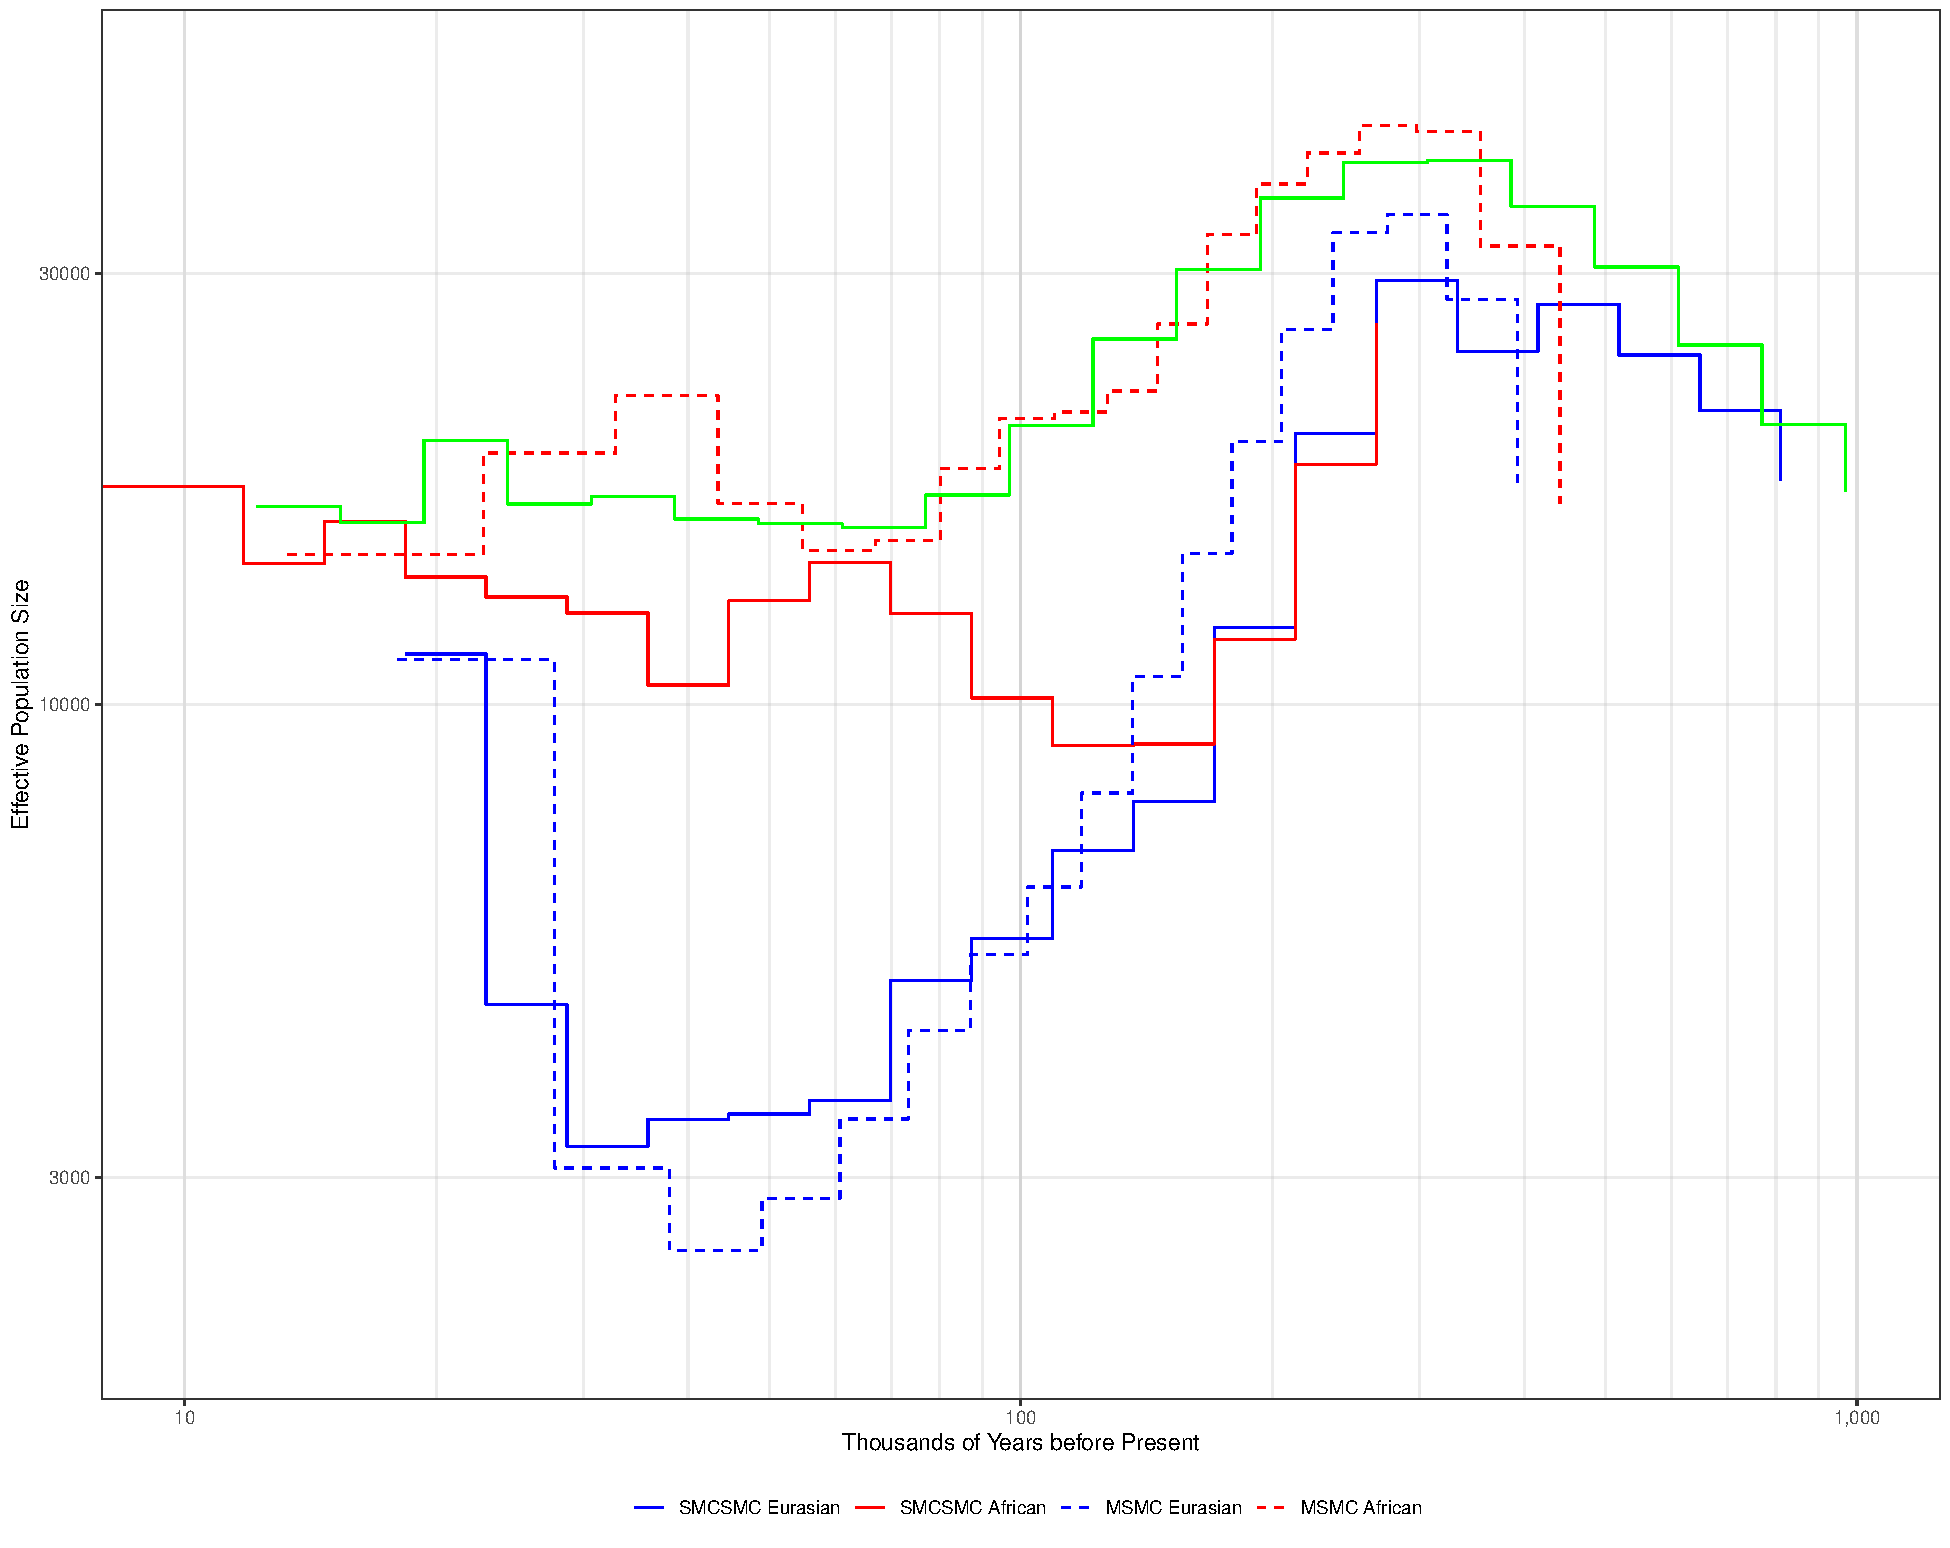
\includegraphics[width=\textwidth]{../plot/ne/figure.pdf}
	\caption{Inferred effective population size using {\tt smcsmc} and MSMC from real and simulated whole genome sequence data. A. Inferred $N_e$ of Han Chinese and Yoruban individuals from the SGDP in both MSMC and {\tt smcsmc}. B. $N_e$ of Han Chinese and Yoruban individuals from the physically phased subset of the HGDP. C, D, and E simulate demographic histories with a 33\%, 42.5\%, and 50\% total replacement 60kya, over the span of 10ky, in {\tt scrm} and reinfer the $N_e$ with {\tt smcsmc}. We replicate a PSMC-like analysis by analysing one diploid Yoruban with {\tt smcsmc} (PSMC$^2$).}
	\label{neplot}
\end{figure}

%In the populations with this trend, {\tt smcsmc} infers directional migration from Eurasian populations to African ones. Specifically, we select a representative from each African population in the Simons Genome Diversity and model migration to a French, Han, and Papuan individual in different analyses. We initialise the inference with a symmetrical migration equal to 1.00 4$N_0$ proportion replaced per generation (henceforth, we assume an $N_0=14312$ {\bf CITE?}), a choice we justify through simulation in Supplemental Simulation \ref{minit}. A comparable magnitude of migration is found in Niger-Kordofanian and Nilo-Saharan populations, while analysis with Afroasiatic populations shows a sustained history of bidirectional migration consistent with the literature. San groups show a lower degree of migration, which is seen to a lesser degree in Mbuti populations. 

\begin{figure}
	\centering
	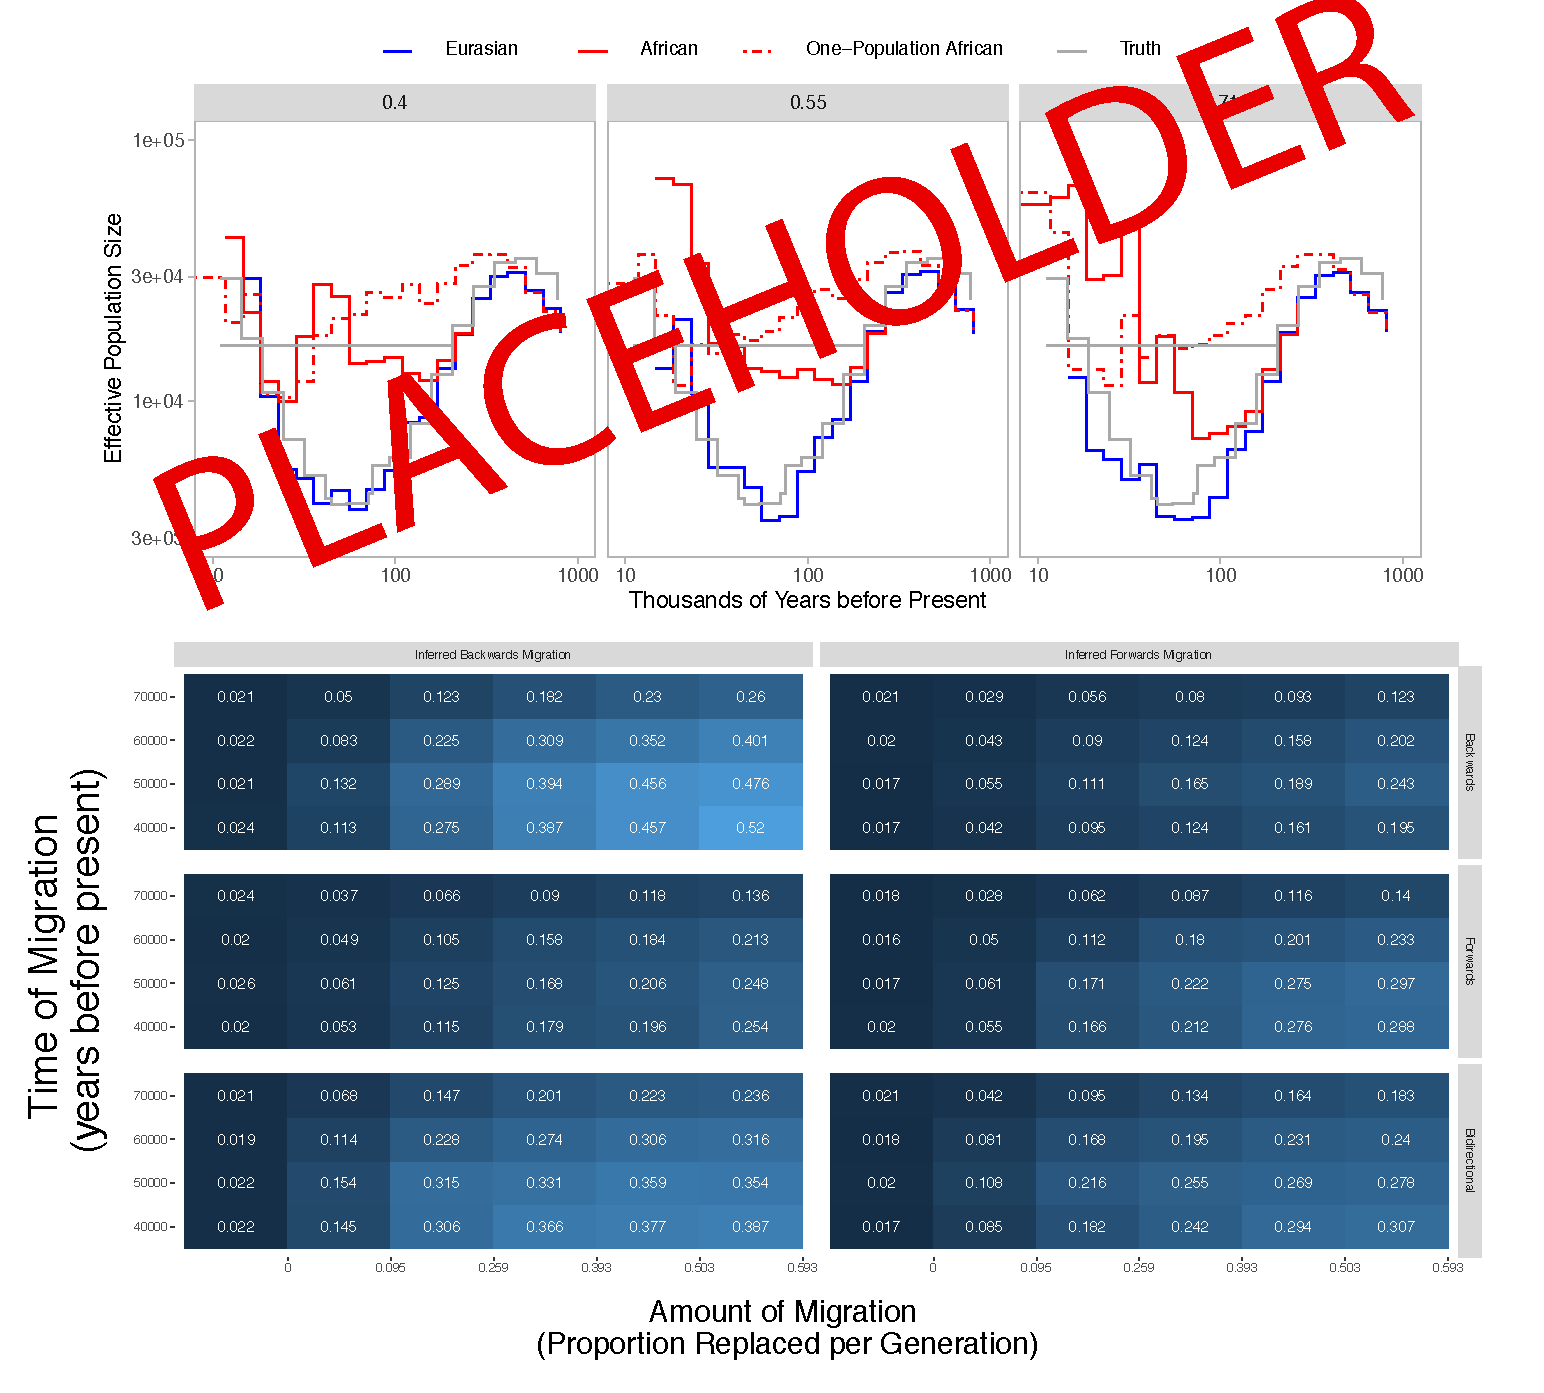
\includegraphics[width=\textwidth]{../plot/ne/PLACEHOLDER_sims.pdf}
	\caption{Top: One gigabase of sequence was simulated by {\tt scrm} under models with increasing migration from an ``African'' population to a ``Eurasian'' population. The magnitude of the population replaced by the migration is indicated in the grey ribbon. In Figure S we additionally vary the timing and duration of the migration, which for this figure are fixed at 60kya and 10ky respectively. Dotted line indicates a single diploid ``African'' genome which was analysed in a one-population model. Grey indicates the true population size simulated. Bottom: Under three different scenarios (migration ``backwards'' from Eurasia to Africa, migration ``forwards'' from Africa to Eurasia, and ``bidirectional'' migration, all forward in time), {\tt scrm} was used to simulate one gigabase of sequence and 5 iterations of {\tt smcsmc} with 5000 particles were used to infer migration. The axis of each heatmap shows increasing simulated proportion replaced over 100,000 while the Y shows the midpoint of the migration simulated. The full migration and population size inference over time along with a more substantial set of simulations is available in Supplemental Section \ref{simproc}.}
	\label{sim}
\end{figure}

\begin{figure}
	\centering
	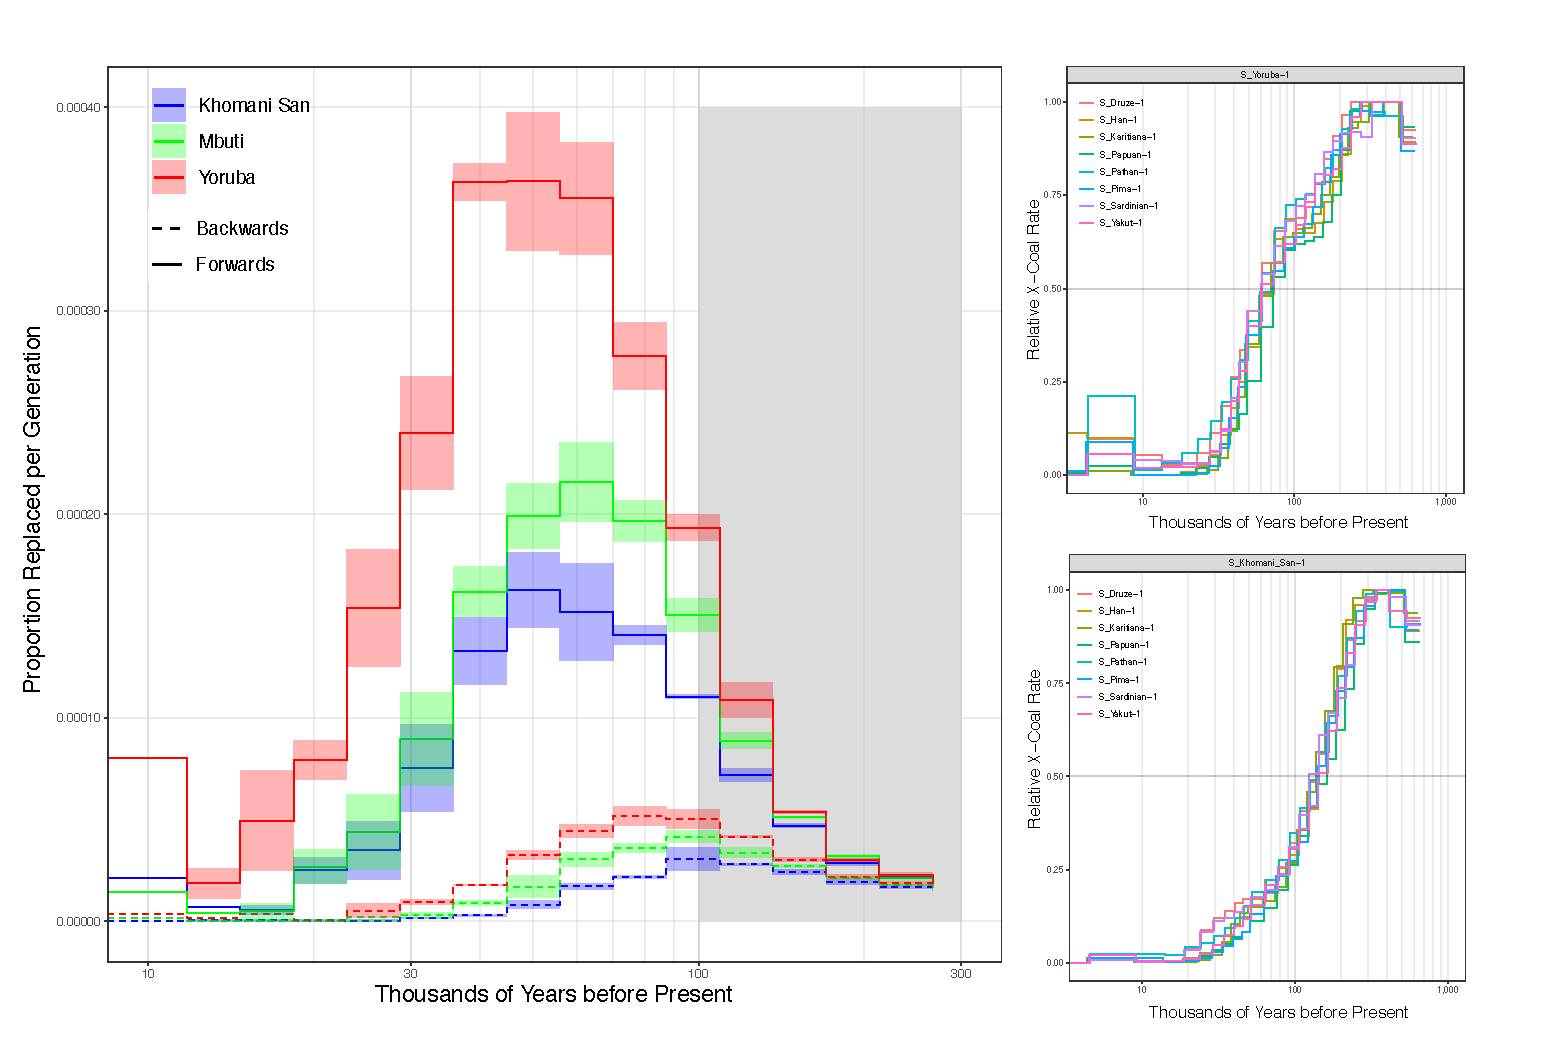
\includegraphics[width=\textwidth]{../plot/mig/mig.pdf}
	\caption{Migration estimates from the Simons Genome Diversity Panel. A. shows three replicates of {\tt smcsmc} inferred migration to with a Han Chinese individual in three contrasting populations representing Niger-Kordofanian and San populations, with the Mbuti a unique intermediate. Analysis used 10000 particles and 25 iterations of variation Bayesian inference to converge. Trend line represents the mean of the replications, while the shaded regions denote the standard deviation. B. and C. show relative cross-coalescent (x-coal) curves for the Yoruban and San individuals modelled with a panel of Out of Africa OoA populations showing contrasting migration histories.}
	\label{migrationplot}
\end{figure}

\begin{figure}
	\centering
	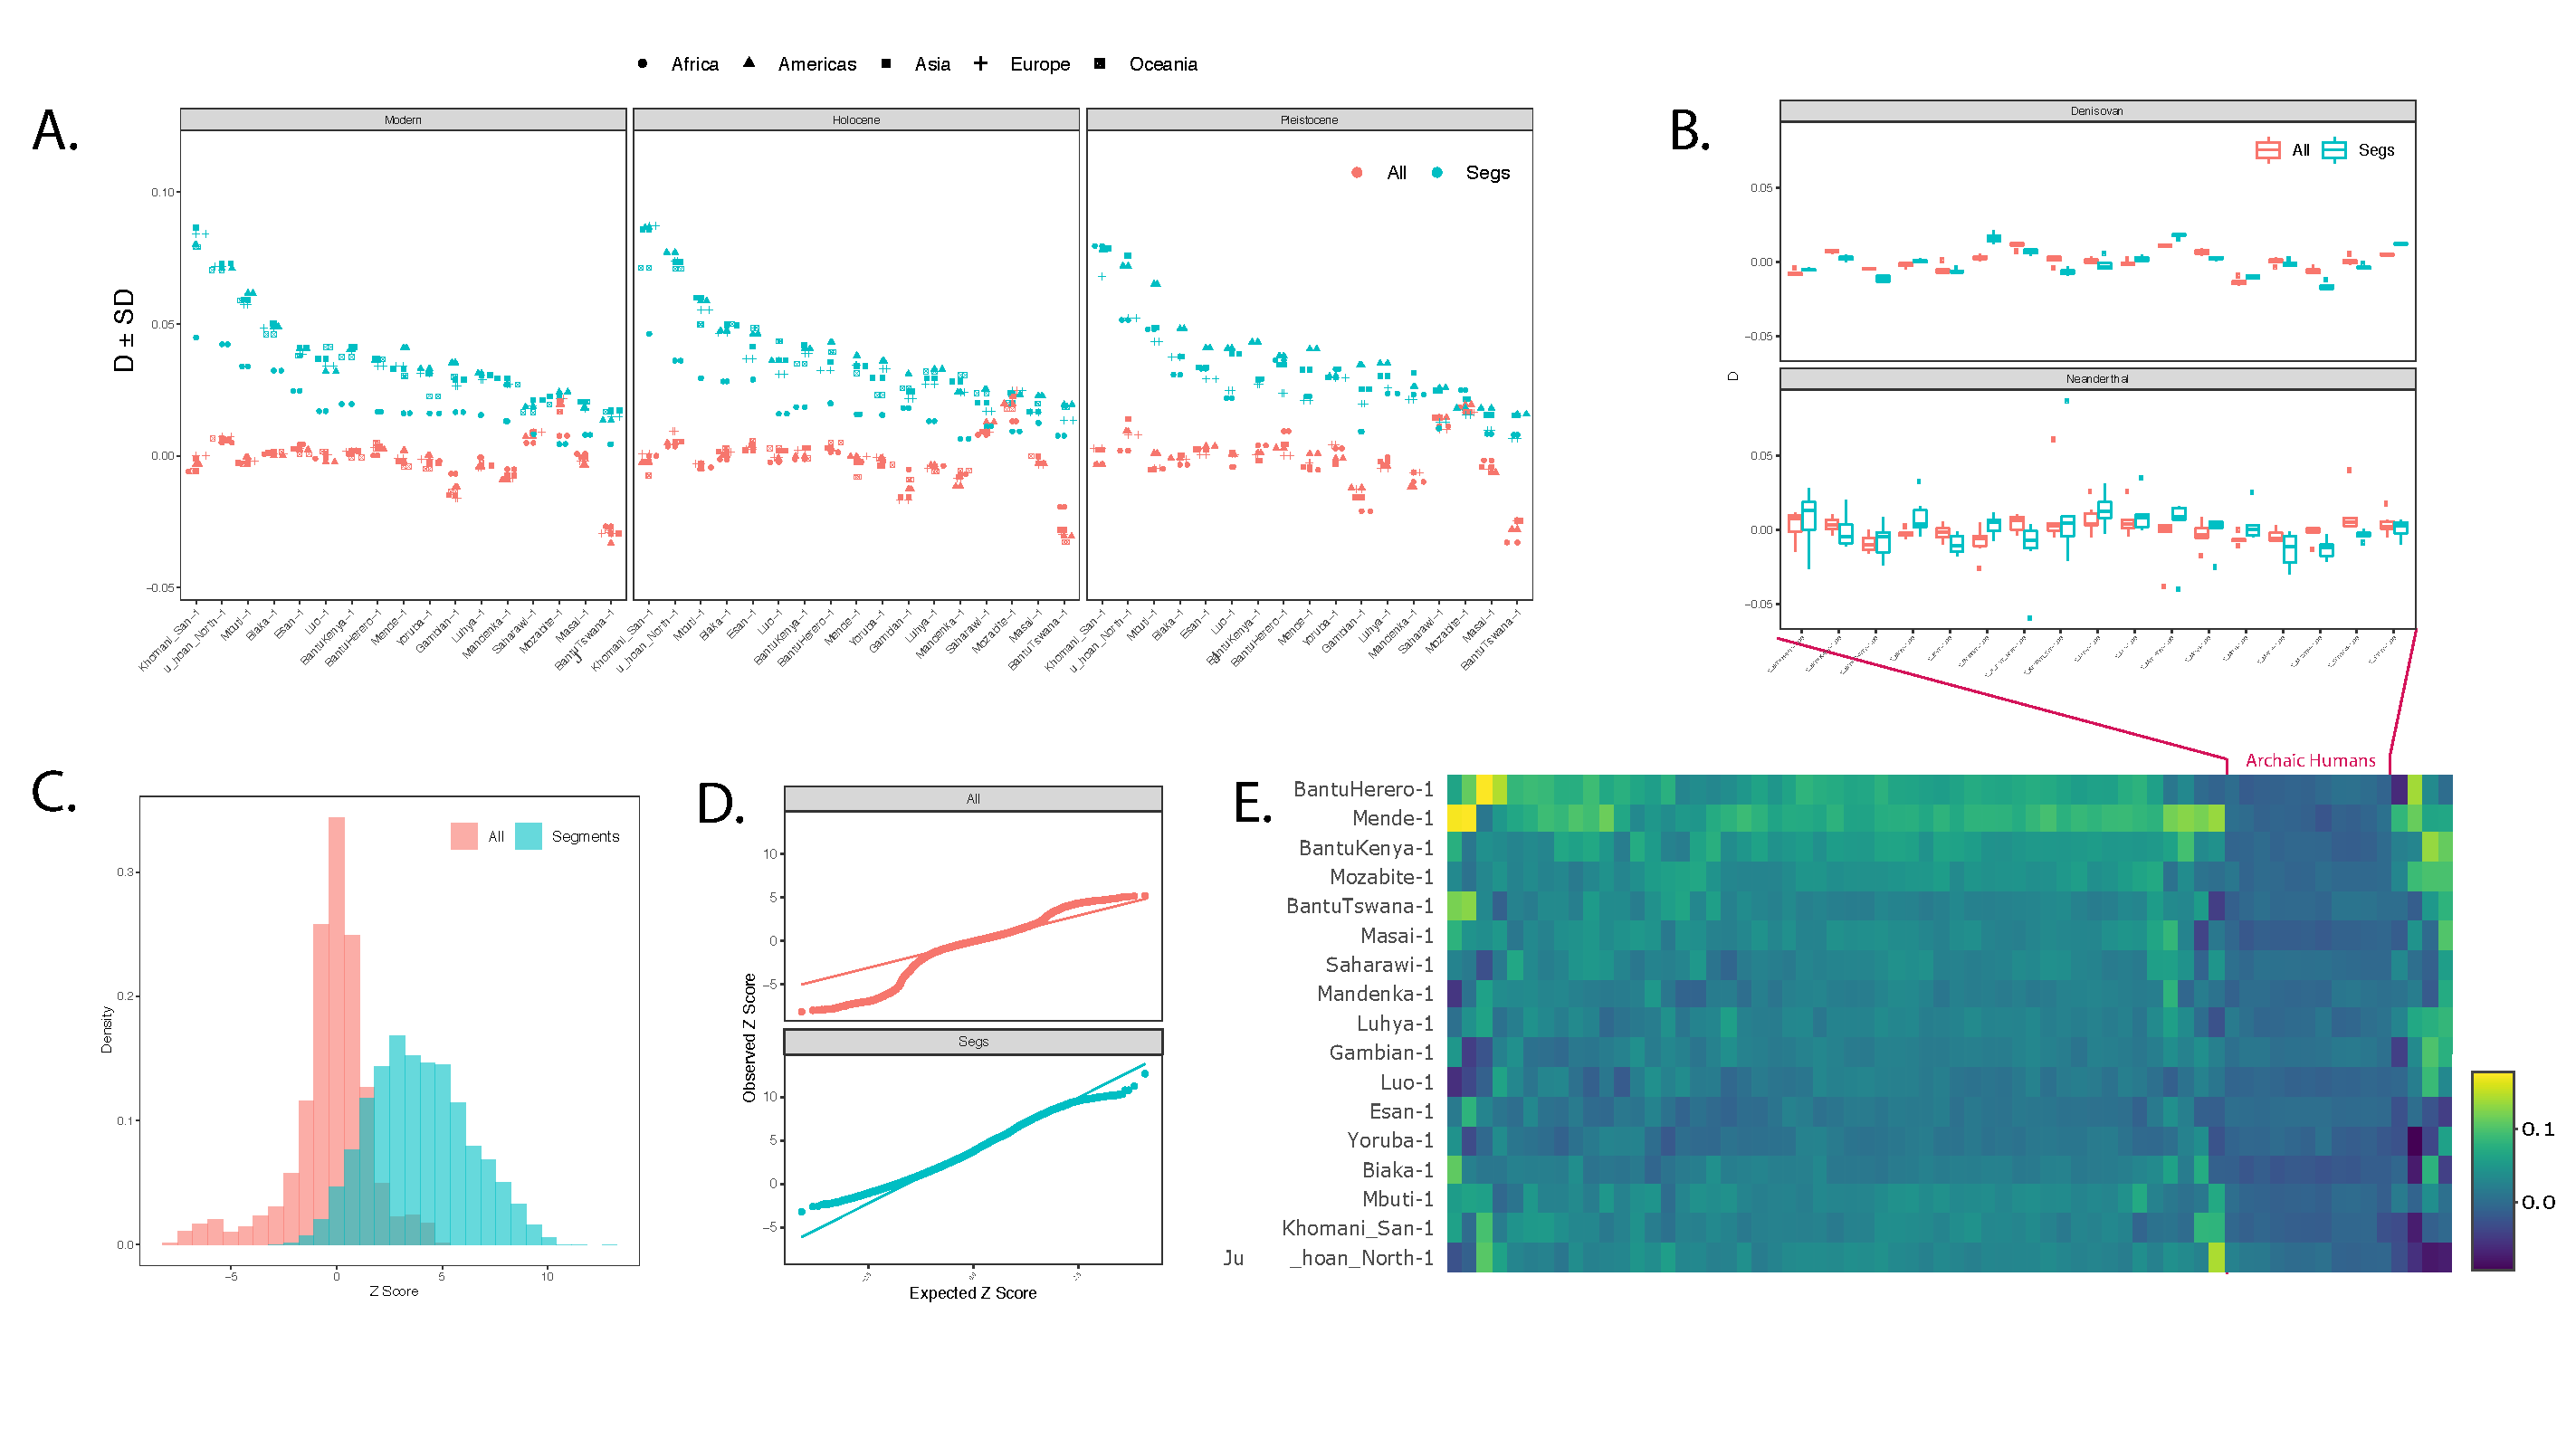
\includegraphics[width=\textwidth]{../plot/dstats.pdf}
	\caption{Analysis of $D(A, A_p, Y, Chimp)$ statistics for all analysed African populations $A$ paired with a partner from the same population $A_p$ and analysed for gene flow with a global population $Y$ from the Reich Lab genotype database. A. compares average $D$ statistic by continent in different African populations, calculated for both all available markers and for the portion of the genome whose tree contains a back-migration event. This is stratified by the age of the comparison sample, either Modern (Present - 1kya), Holocene (1kya - 11.7kya), or Pleistocene ($>11.7$kya). B. displays the distribution of $D$ statistics for both sections, while C. gives a QQ plot of their Z statistics. D. shows a heatmap of D statistics for all of the Pleistocene samples, with E. being a blow-out of the Denisovan and Neanderthal statistics.}
	\label{dstats}
\end{figure}


\begin{figure}
	\centering
	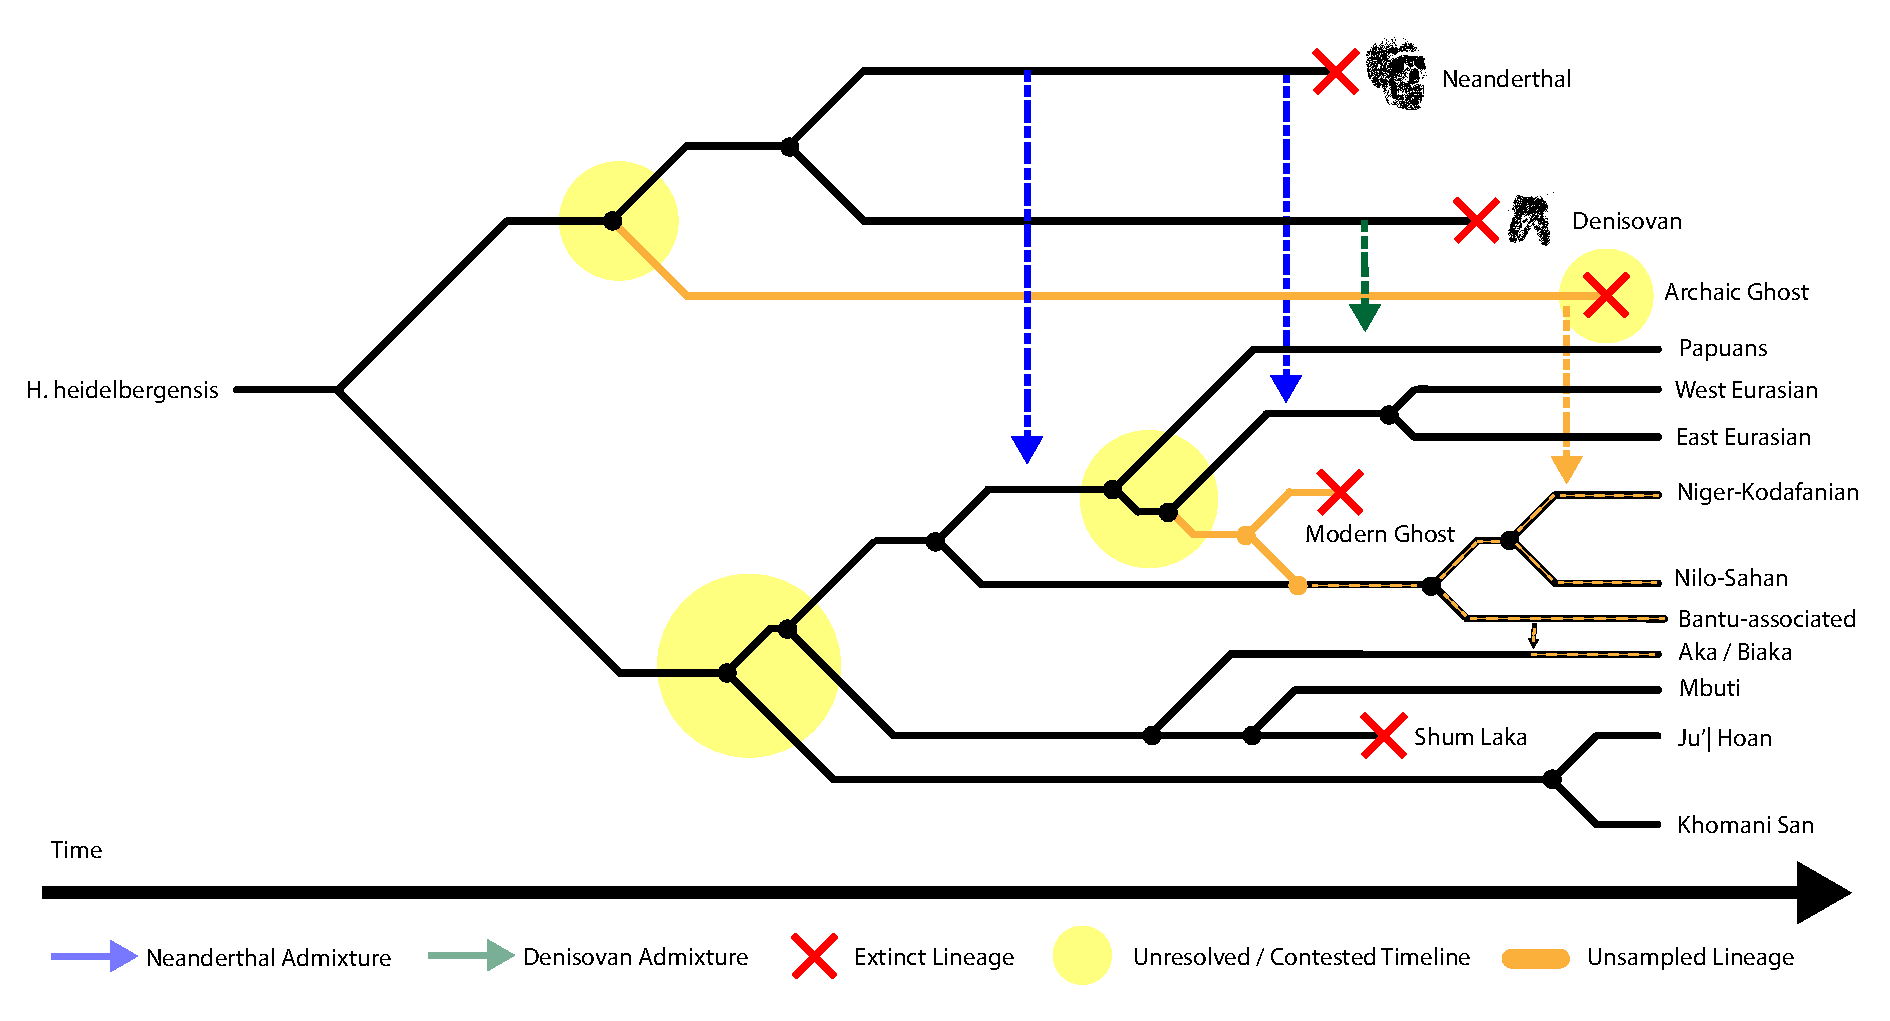
\includegraphics[width=\textwidth]{../plot/dem2.pdf}
	\caption{Proposed Demographic Model. Population splits coloured in yellow are contested. The existance of an archaic ghost lineage which has contributed to Western African populations has been broadly supported in the literature, but the time and order of divergences relative to Neanderthals and Denisovans remains an open question. Until recently, the San peoples were considered to be the most anciently diverged group in Africa, though recent evidence places Central African Hunter Gatherers on a similar timespan, with the addition of a modern ghost population. This existance of this population is additionally supported in the literature and in this article, though the order of divergence is contested. In this article we posit that the ghost diverged from the common ancestor of Eurasians after Papuans had diverged, similar to that suggested in \cite{Malaspinas2016}.}
	\label{fig_dem}
\end{figure}

%\subsection*{URLs}
%\paragraph{Simons Genome Diversity Panel Phased Release} \url{https://sharehost.hms.harvard.edu/genetics/reich_lab/sgdp/phased_data/}
%\paragraph{Human Genome Diversity Panel} \url{ftp://ngs.sanger.ac.uk/production/hgdp/hgdp_wgs.20190516/}
%\paragraph{Ancient DNA} \url{http://cdna.eva.mpg.de/neandertal/}
%\paragraph{Strict 1000 Genomes Accessibility Mask} \url{ftp://ftp.1000genomes.ebi.ac.uk/vol1/ftp/release/20130502/supporting/accessible_genome_masks/}
%\paragraph{SMCSMC Implementation} \url{https://github.com/luntergroup/smcsmc}
%\paragraph{vcf2eigenstrat} \url{https://github.com/bodkan/vcf2eigenstrat}
%\paragraph{ADMIXTOOLS} \url{https://github.com/DReichLab/AdmixTools}
%\paragraph{admixr} \url{https://github.com/bodkan/admixr}



\newpage
\emergencystretch=1em
\printbibliography

\newpage
\setcounter{section}{0}
\renewcommand{\thesection}{S\arabic{section}}%
\setcounter{table}{0}
\renewcommand{\thetable}{S\arabic{table}}%
\setcounter{figure}{0}
\renewcommand{\thefigure}{S\arabic{figure}}%


\section{Details of Data Analysis}

\subsection{Inferring population size and migration rates in the Simons Genome Diversity Panel}

This section describes analysis of the Simons Genome Diversity Panel with both {\tt smcsmc} and MSMC. {\tt smcsmc} version 1.0.1 was installed from the conda package manager (also found at \url{https://github.com/luntergroup/smcsmc/releases/tag/v1.0.1}), MSMC version 1.1.0 was installed from Github (found at \url{https://github.com/stschiff/msmc/releases/tag/v1.1.0}) and all analyses were performed on the Oxford Biomedical Research Computation cluster.

We download prephased sequencing data from \url{https://sharehost.hms.harvard.edu/genetics/reich_lab/sgdp/phased_data/} and mask for the strict accessibility mask from the 1000 genomes project. We additionally mask for any sites absent Chimpanzee ancestry due to a known issue with the phasing algorithm. We do this masking in {\tt vcftools}. We use {\tt smcsmc} to convert the sequence data from VCF to seg file format, a format very similar to MSMC format. We provide a script to convert from seg file format to MSMC file format as well. Unless otherwise noted, the names of individuals used in this paper are the first in their population (i.e. an individual named Yoruban is {\tt S\_Yoruba-1} in the SGDP nomenclature). We select two diploid individuals from each population in Africa  and infer piecewise constant population size and directional migration rates. Specifically, we use the following options for {\tt smcsmc}:

\begin{verbatim}
smc2 -c -chunks 100 -no_infer_recomb -nsam 4 -I 2 2 2
-mu 1.25e-8 -rho 3e-9 -calibrate_lag 1.0 -EM {EM} 
-tmax 3.5 -alpha 0.0 -apf 2 -N0 14312 -Np {Np} -VB 
${DEMOGRAPHIC_MODEL} -P 133 133016 31*1 
-arg -o ${OUTPUT} -segs ${SEGS}
\end{verbatim}

In order, we invoke the use of a QSUB cluster with {\tt -c} and split our analysis into 100 chunk. We do not infer recombination sites along with the demographic model in order to reduce runtime. Four haploid samples, two from each population, are analysed with a mutation rate of 1.25 $\times 10^{-8}$, a recombination rate of 3 $\times 10^{-9}$, and accumulating events for one unit of survival time along the sequence. We use a given number of epochs for parameter units, and bound the upper limits of the trees at 3.5 times the effective population size (set to 14312). We use the lookahead likelihood to guide the resampling process for a given number of particles {\tt Np} and use variational Bayes in place of the default stochastic expectation maximization algorithm. Parameters are inferred over 31 equally spaced intervals from 133 to 133016 generations in the past, and the sampled posterior ARGs are reported. 

We seed the particle filter with a demographic model of population size and uniform symmetric migration rate, given by the following {\tt scrm} command:

\begin{verbatim}
-ej 0.2324 2 1 -eM 0 1 -eN 0.0 6 -eN 0.0037 4.4 -eN 0.0046 3 
-eN 0.0058 2 -eN 0.0073 1.4 -eN 0.0092 0.85 -eN 0.093 1.2 
-eN 0.12 1.7 -eN 0.15 2.2 -eN 0.19 2.5 -eN 0.24 2.4 -eN 0.30 2.0 
-eN 0.37 1.7 -eN 0.47 1.4 -eN 0.59 1.2 -eN 0.74 1.0 
-eN 0.93 0.91 -eN 1.2 1.6
\end{verbatim}

We visualise this demographic model in the POPdemog package in Figure \ref{smc2demog}.

\begin{figure}
	\centering
	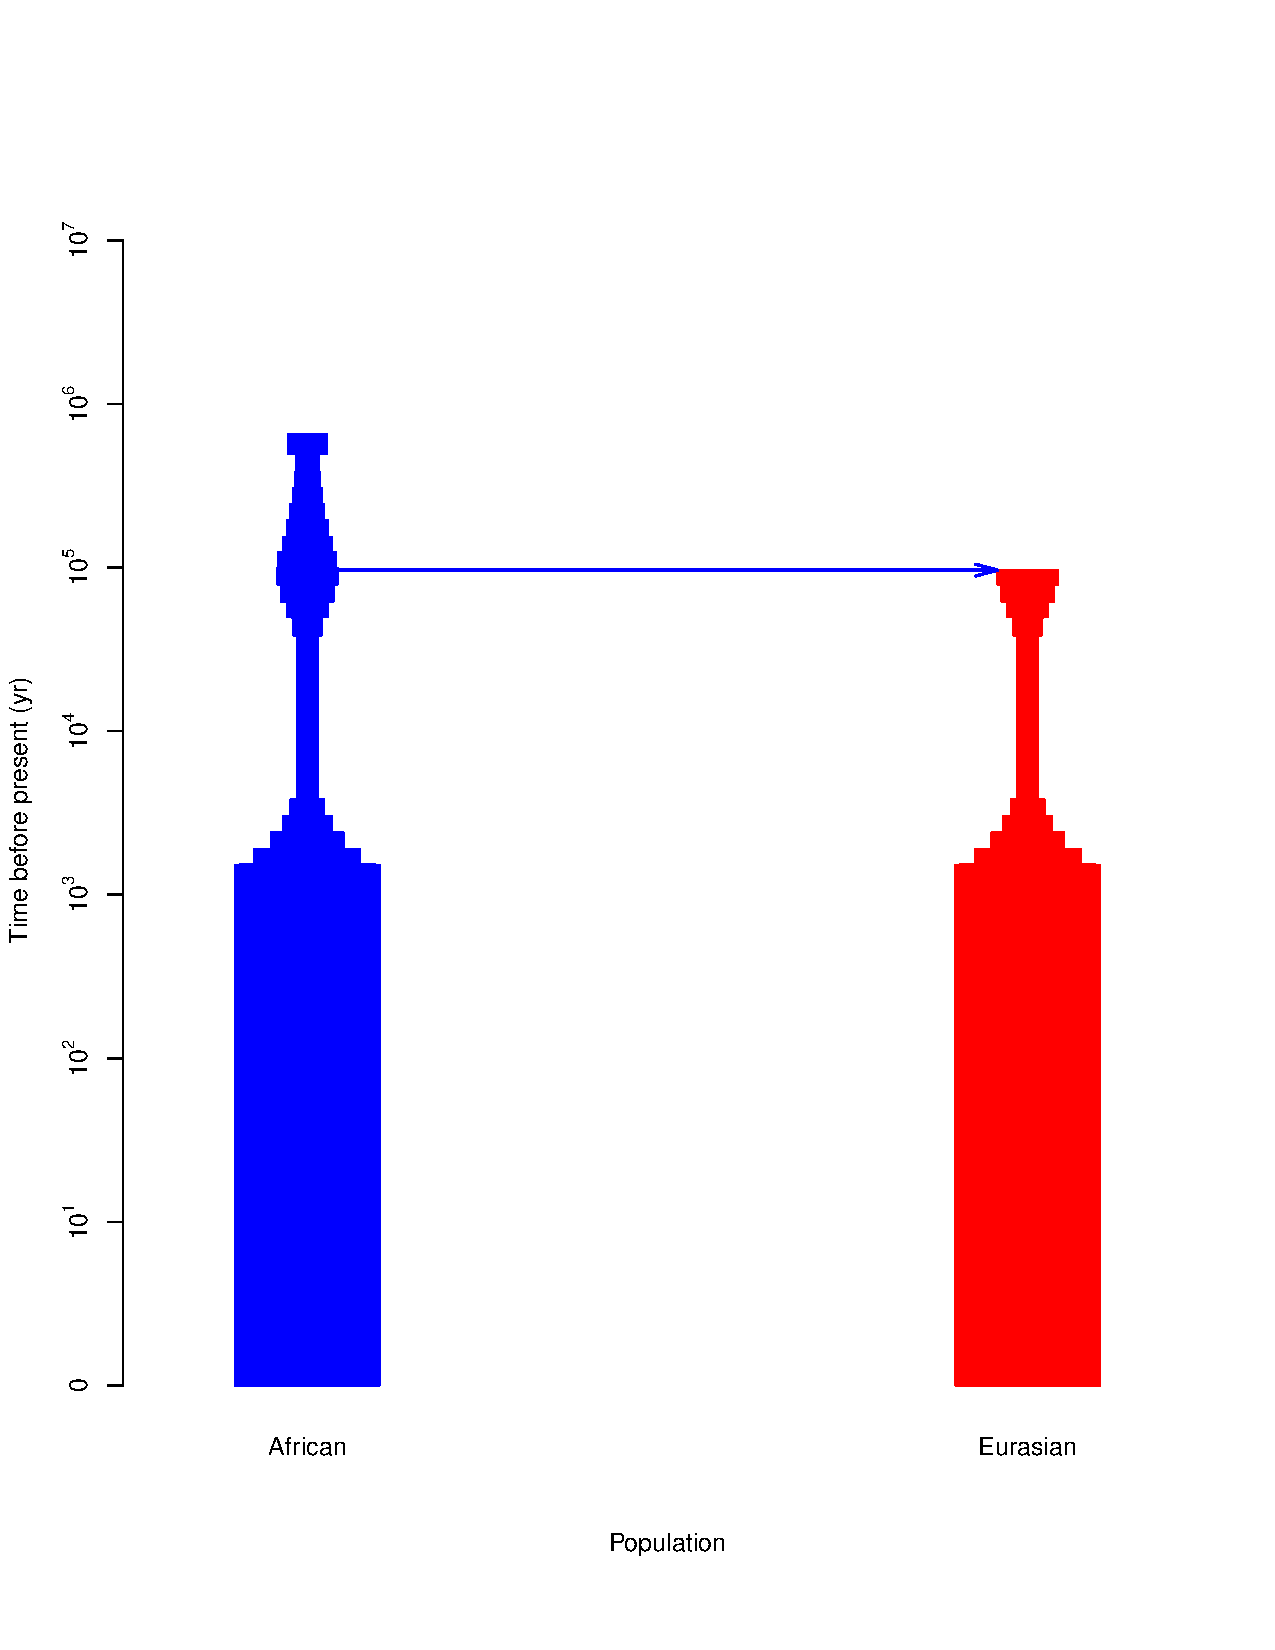
\includegraphics[width=0.25\textwidth]{../plot/dem_smc2.pdf}
	\caption{Demographic model used as a seed for SMC2 analysis}
	\label{smc2demog}
\end{figure}

Each {\tt smcsmc} analysis gives a final output file detailing migration and coalescent events, their rates, and their opportunities which denote the total opportunity for an event to occur during a particular epoch. Output files are trimmed to only visualise the final epoch of variational Bayes inference and assessed for convergence. Times and rates are interpreted differently than {\tt scrm} output. Rates are in units of $4N_0$ per generation, while times are given in generations. 

We implement the above in an open source {\tt Snakemake} pipeline at \url{SNAKEM} which also implements a default analysis of MSMC with forty iterations to converge. Sample size and relative cross-coalescent rates are transformed as described in the documentation using the same parameter values for mutation rate and generation time used for {\tt smcsmc} analysis. Effective population size and migration estimates for the populations analysed in the SGDP are given in Figures \ref{sgdp_ne} and \ref{sgdp_mig}. MSMC appears to consistently find a higher African $N_e$ in the ancient past until the average estimates across populations stabalises approximately 100kya (Figure \ref{averages}). We expand on a possible rational behind this effect in the main text of this article.

\begin{figure}
	\centering
	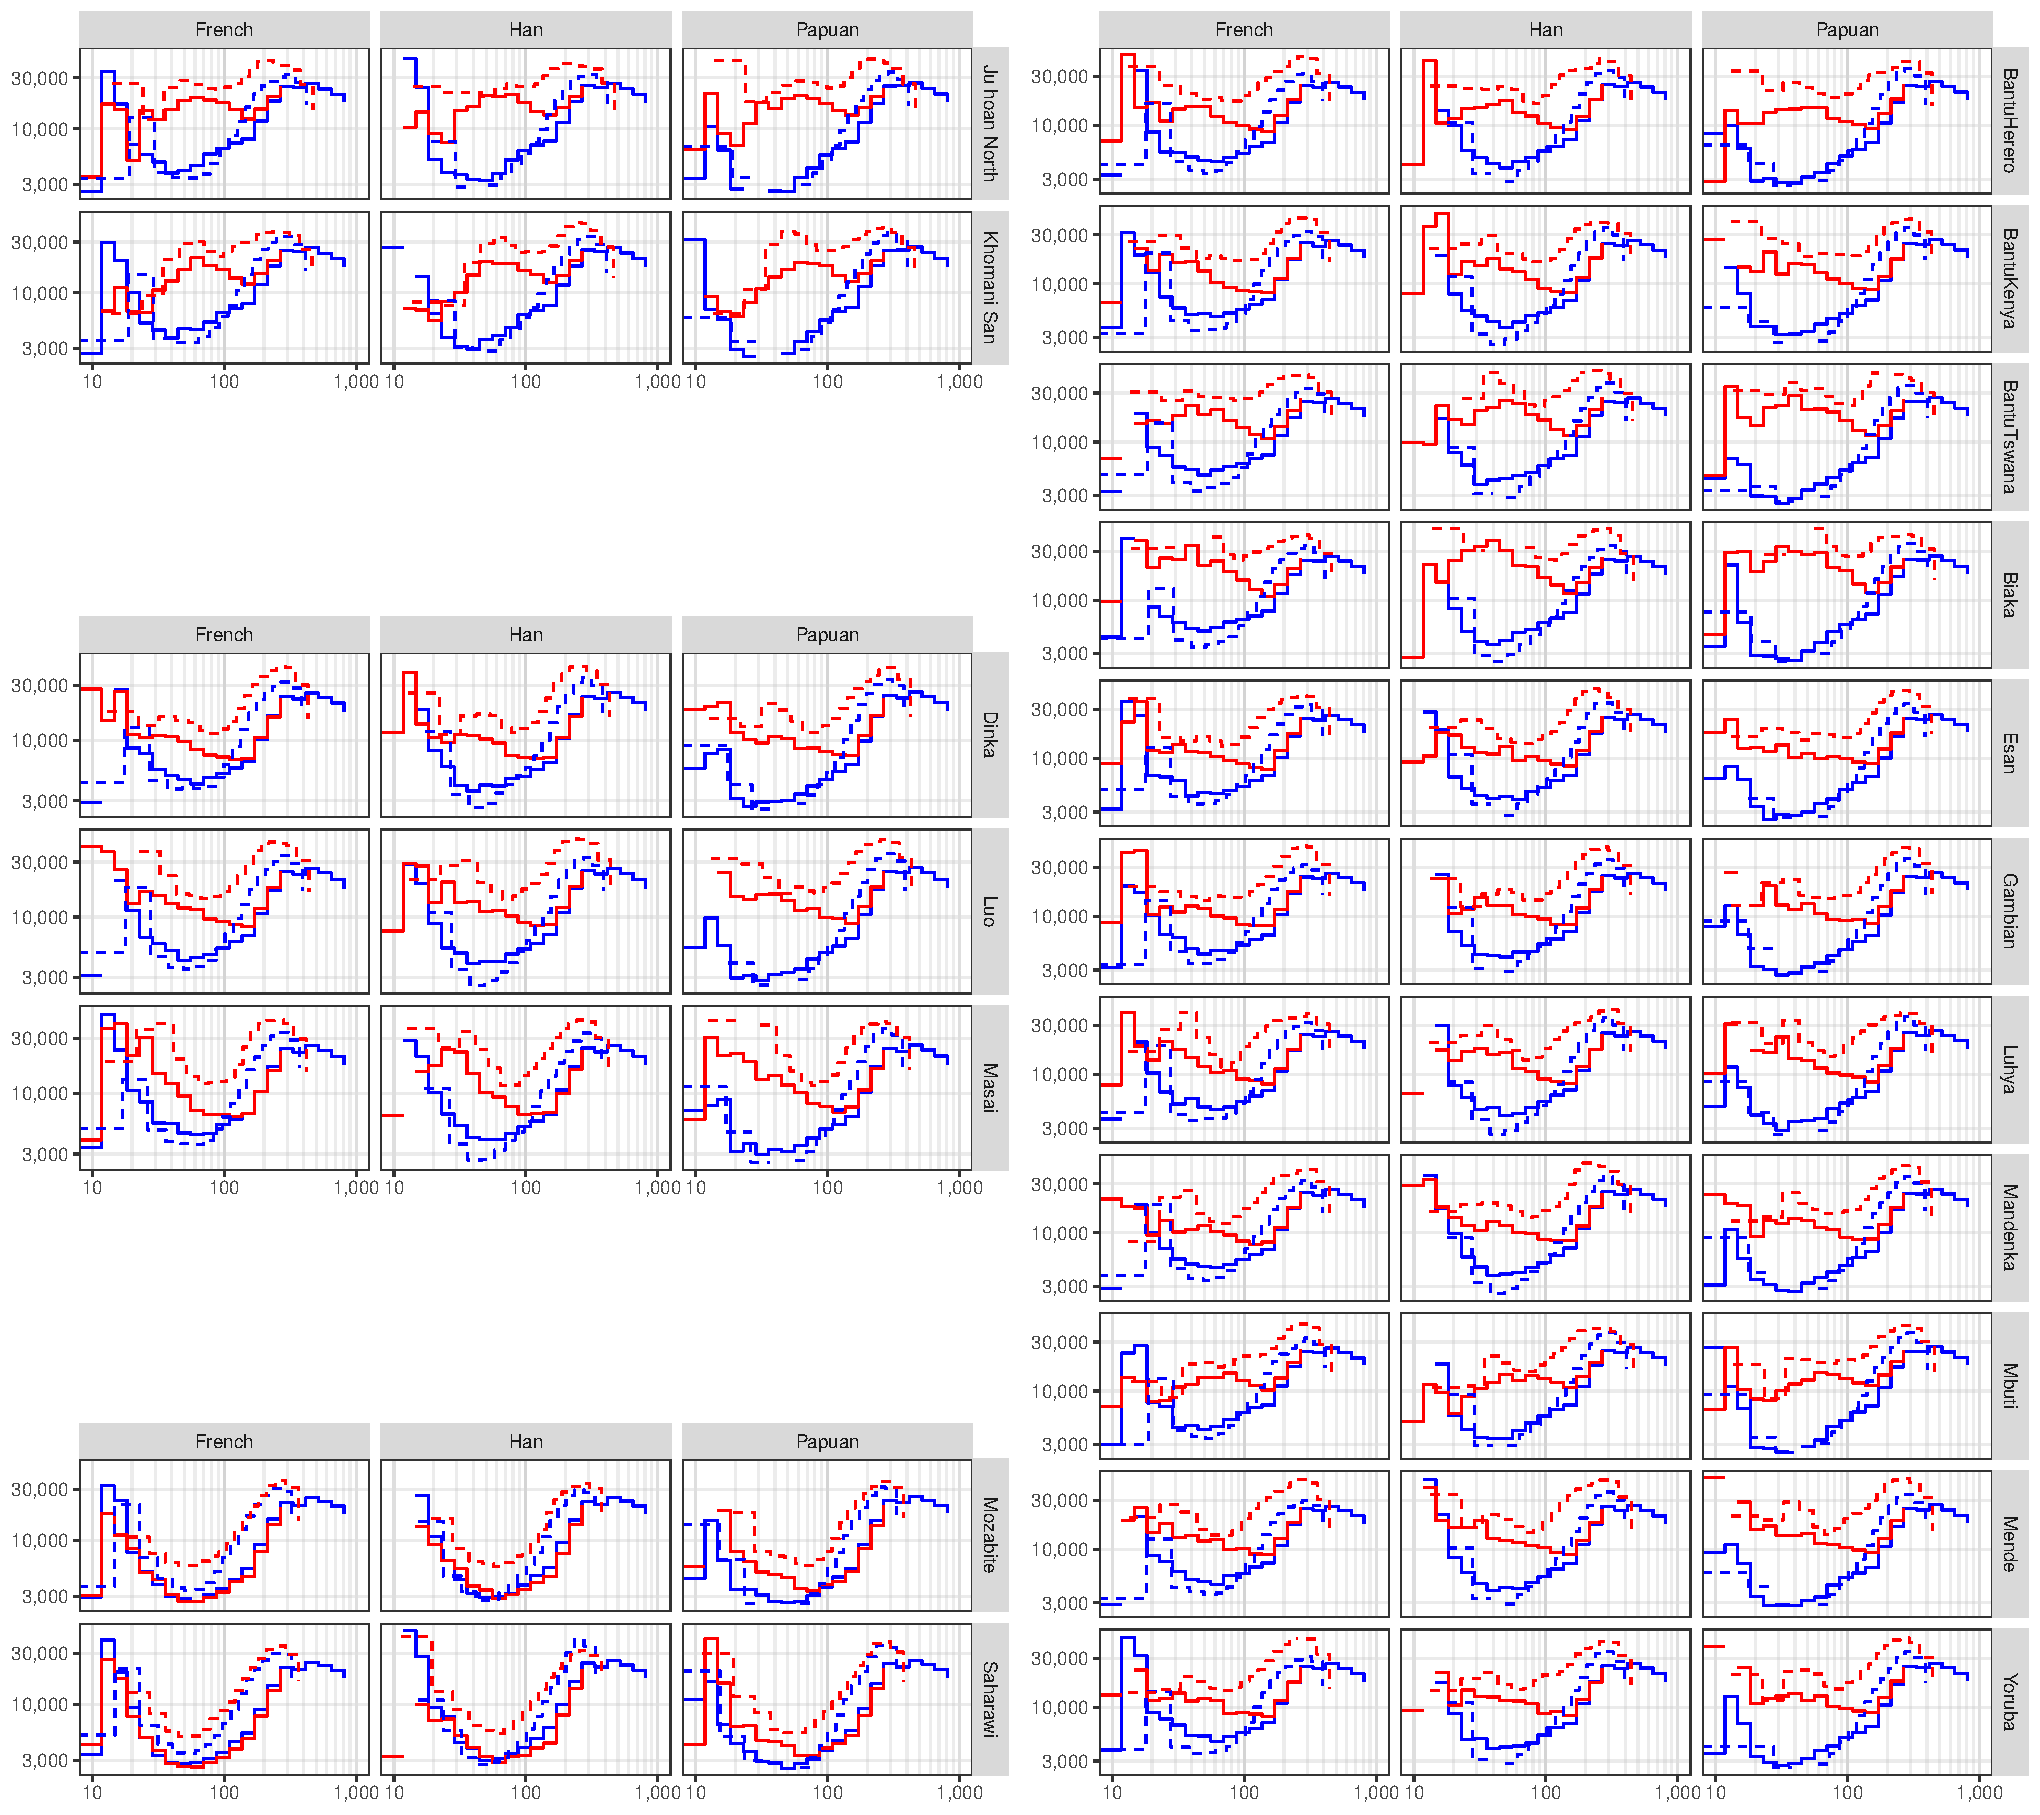
\includegraphics[width=0.75\linewidth]{../plot/sgdp_ne.pdf}
	\caption{Estimated effective population size in different African and Eurasian groups with {\tt smcsmc}. Left: From top to bottom, inferred $N_e$ in Khoesan, Nilo-Saharan, and Afroasiatic populations. Right: Inferred $N_e$ in Niger-Kordofanian populations. 5000 particles and 10 variational Bayes interations were used to achieve convergence.}	
	\label{sgdp_ne}
\end{figure}

\begin{figure}
	\centering
	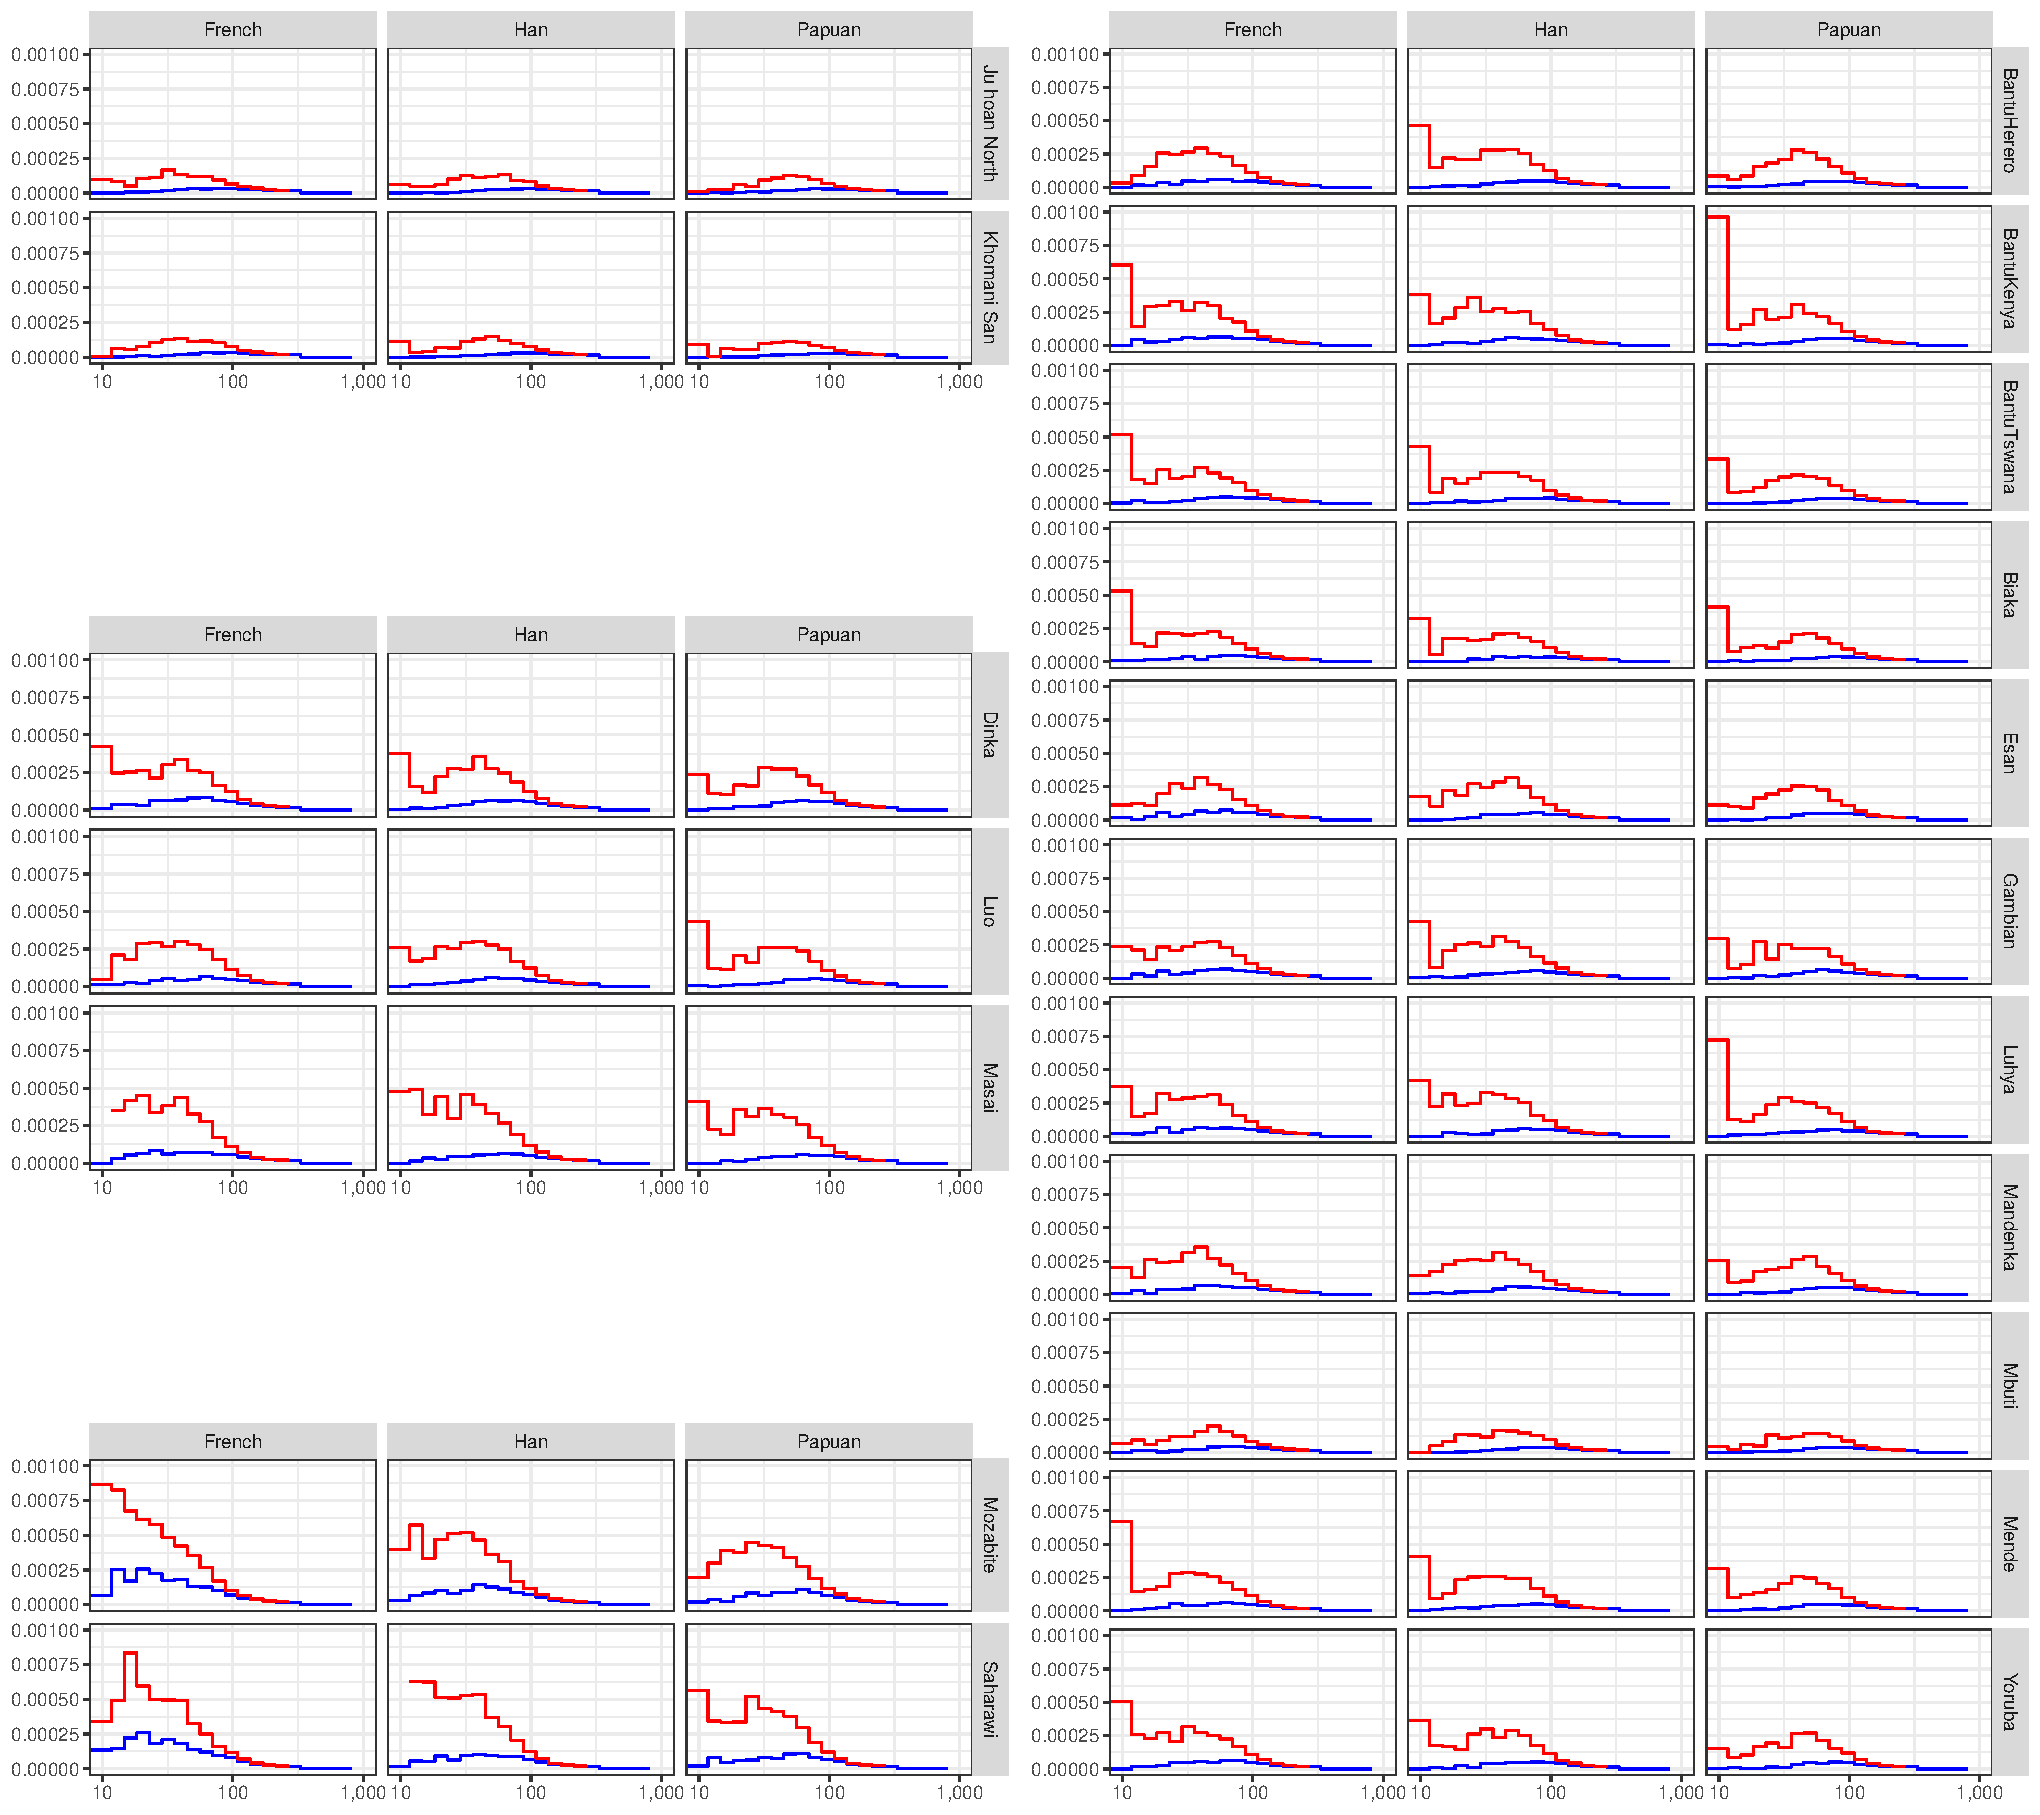
\includegraphics[width=0.75\linewidth]{../plot/sgdp_mig.pdf}
	\caption{Estimated directional migration between African and Eurasian groups in the SGDP with {\tt smcsmc}. Left: From top to bottom, inferred migration in Khoesan, Nilo-Saharan, and Afroasiatic populations. Right: Inferred migration in Niger-Kordofanian populations. 5000 particles and 10 variational Bayes interations were used to achieve convergence.}	
	\label{sgdp_mig}
\end{figure}

\begin{figure}
	\centering
	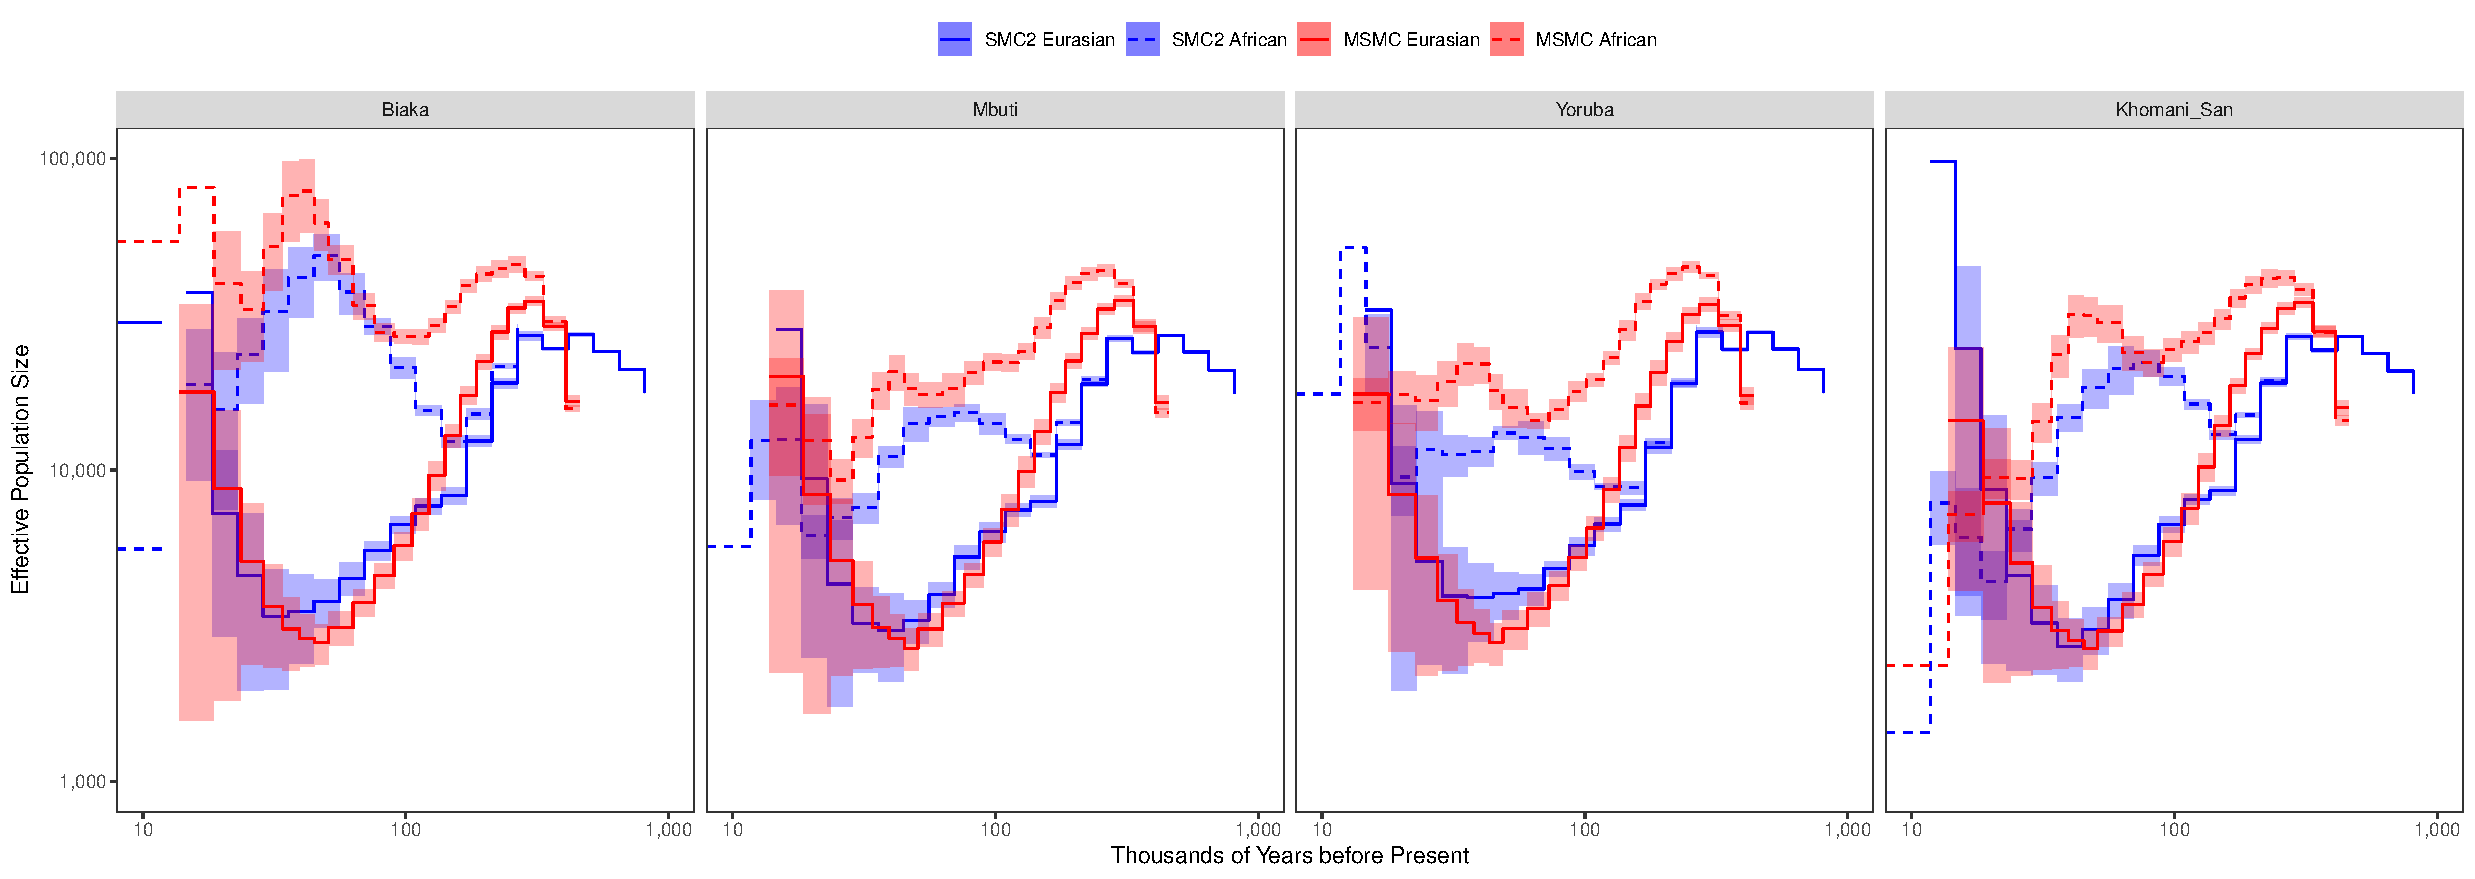
\includegraphics[width=\textwidth]{../plot/ne/average_ne_subset.pdf}
	\caption{Average $N_e$ estimate across four populations in the subset of SGDP used to compare with HGDP inference. Inference of population size is averaged over eight Eurasian populations, with the bars representing standard deviation. For MSMC, the time indexes were averaged to have consistent start and stop times for the steps.}
	\label{averages}
\end{figure}

Migration during the last 100ky is integrated to observe overall trends (Figure \ref{sgdp_heatmap}). We use two methods to integrate migration, the first presented in the main text given by $F(t) = e^{- \int_{t=0}^T \rho(t) dt}$. Alternatively, consider $p$ proportion of the population are replaced every generation. Start with 0 individuals from the source $N_{source}$ population in the sink population $N_{sink}$, each generation replace $p$ proportion of the sink population with the source. We track the proportion of the population which are replaced by the source $P$.  

$$ \begin{aligned} P_0 &= 0 \\ P_1 &= pN_{sink} \\ P_2 &= pN_{sink} + p(N_{sink} - pN_{sink}) \\ &= pN_{sink} + pN_{sink}(1-p) \\ P_3 &= pN_{sink} + pN_{sink}(1-p) + p((N_{sink}-pN_{sink}) - p(N_{sink}-pN_{sink})) \\ &= pN_{sink} + pN_{sink}(1-p)+p(N_{sink}(1-p)-pN_{sink}(1-p)) \\ &= pN_{sink}+pN_{sink}(1-p)+pN_{sink}(1-p)(1-p) \\ &\dots \\ P_n &=N_{sink}p(1-p)^n \end{aligned} $$

In practice, both methods give essentially identical proportions for all considered questions. Inferred migration varies across language groups (Figure \ref{averages_of_sgdp}. Afroasiatic groups show high migration from Han and French populations, with a lower proportion deriving from Papuans. Niger-Kordofanian and Nilo-Saharan groups show an intermediate magnitude, between 50 and 60 percent replacement, though also significantly (P < 0.05, two-tailed paired $T$ test) closer to French and Han sources than Papuans. The Khoesan show the lowest migration, consistent with their early diversification from the remainder of African groups and the relative lack of gene-flow from Western African populations \cite{Lipson2019}. This is contrasted with the Mbuti and Biaka, Central African Hunter Gatherer populations who have historically recieved substantial amounts of gene flow from Western African sources. Both of these populations show the lowest migration in their language group (Table \ref{average_sgdp_migration_table}). 

\begin{figure}
	\centering
	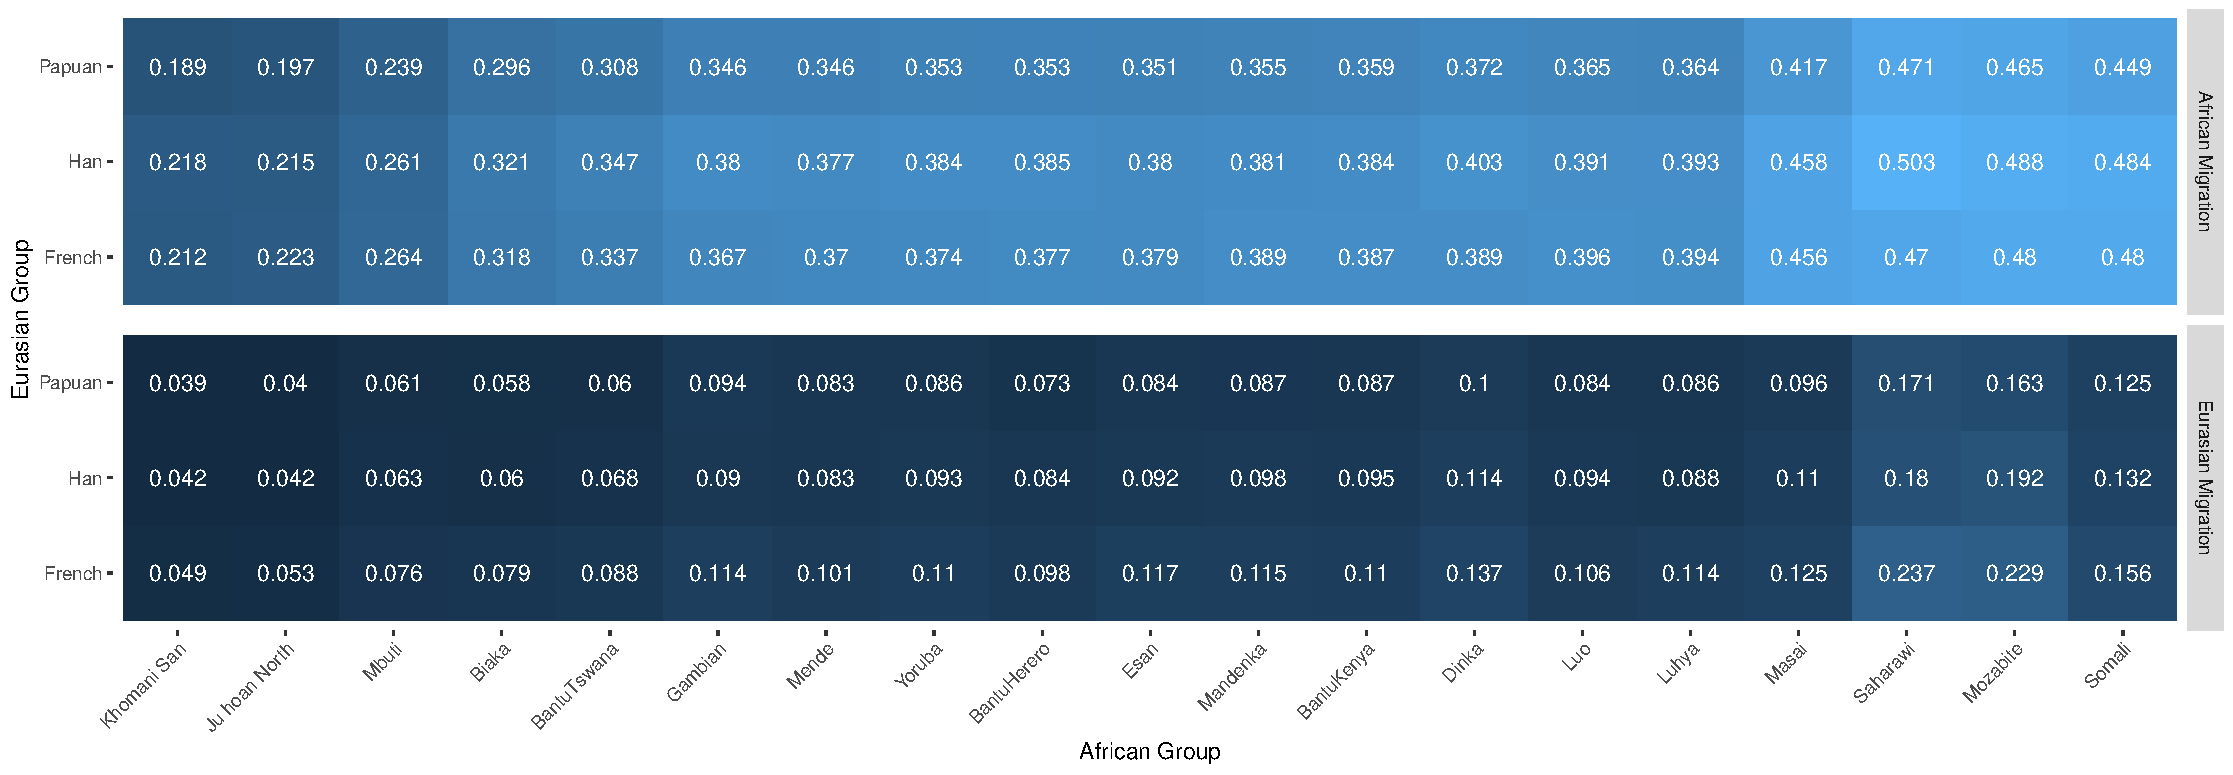
\includegraphics[width=\textwidth]{../plot/mig/integrated_sgdp.pdf}
	\caption{Integrated migration proportion in {\tt smcsmc} analysed SGDP populations.}
	\label{sgdp_heatmap}
\end{figure}

\begin{figure}
	\centering
	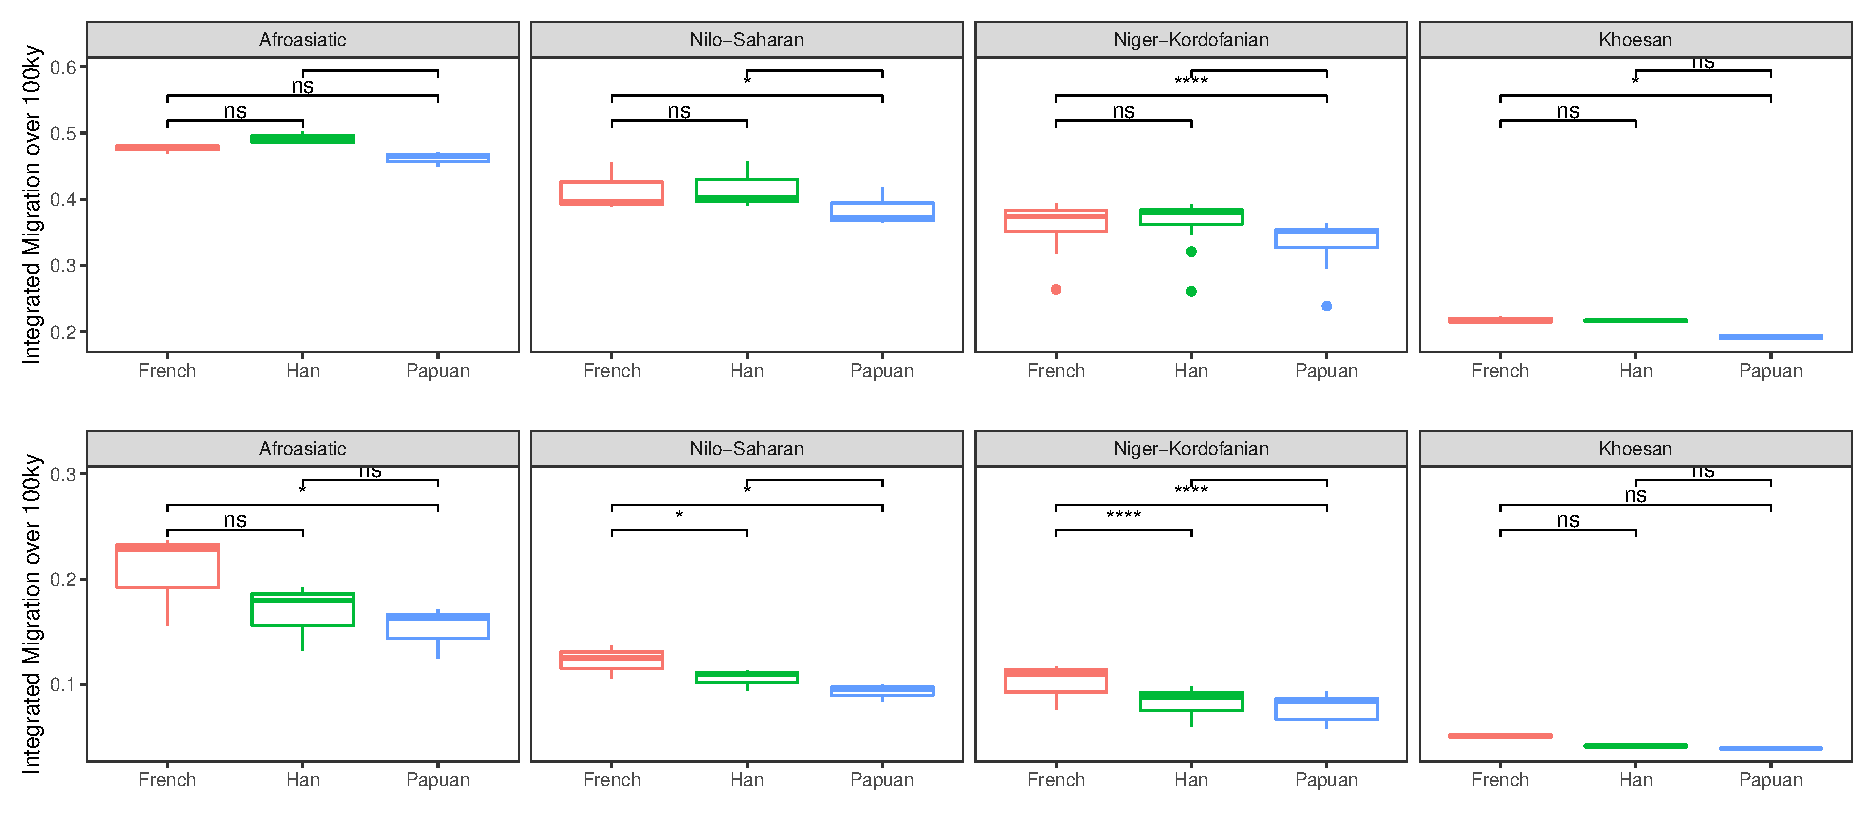
\includegraphics[width=\textwidth]{../plot/mig/sgdp_averages.pdf}
	\caption{Integrated migration proportion over the last 100 thousand years (ky) between language families by comparison population. Papuans contributed significantly less to African populations across all populations in a two tailed paired T test. ns = Not Significant, * = $P<0.05$, ** = $P<0.01$, *** = $P<0.001$, **** = $P<0.0001$.}
	\label{averages_of_sgdp}
\end{figure}

% latex table generated in R 3.5.3 by xtable 1.8-3 package
% Wed Jan 22 11:49:06 2020
\begin{table}[ht]
	\centering
	\begin{tabular}{llll}
		\hline
		African & Eurasian & $M_{E, A}$ (SD) & $M_{A, E}$ (SD) \\ 
		\hline
		Afroasiatic & French & 0.722(0.014) & 0.351(0.092) \\ 
		Afroasiatic & Han & 0.721(0.029) & 0.241(0.055) \\ 
		Afroasiatic & Papuan & 0.642(0.018) & 0.218(0.043) \\ 
		Khoesan & French & 0.304(0.005) & 0.079(0.006) \\ 
		Khoesan & Han & 0.292(0.002) & 0.065(0.004) \\ 
		Khoesan & Papuan & 0.257(0.001) & 0.063(0.004) \\ 
		Niger-Kordofanian & French & 0.514(0.059) & 0.151(0.024) \\ 
		Niger-Kordofanian & Han & 0.513(0.061) & 0.121(0.016) \\ 
		Niger-Kordofanian & Papuan & 0.462(0.059) & 0.114(0.016) \\ 
		Nilo-Saharan & French & 0.595(0.079) & 0.186(0.028) \\ 
		Nilo-Saharan & Han & 0.581(0.055) & 0.152(0.012) \\ 
		Nilo-Saharan & Papuan & 0.525(0.048) & 0.134(0.014) \\ 
		\hline
	\end{tabular}
	\caption{Average plus or minus standard deviation integrated directional migration from Eurasian to African populations in the last 100 thousand years (ky)} 
	\label{average_sgdp_migration_table}
\end{table}

\subsection{Validation in a physically phased subset of the Human Genome Diversity Panel (HGDP)} \label{hgdp_section}

For the {\tt smcsmc} algorithm, the use of phase is not necessary but does help convergence. It additionally helps the lookahead-likelihood to better guide the resampling procedure. Therefore, we do not expect errors made during statistical phasing to significantly impact the inferred parameters. However, to test this, we replicate the above analysis in a physically phased subset of the HGDP downlaoded from \url{ftp://ngs.sanger.ac.uk/production/hgdp/hgdp_wgs.20190516/}. The same {\tt snakemake} pipeline is used as in the analysis of the SGDP data. Data is additionally masked for the filters provided. We plot the effective population size and migration rates in Figures BLAH and BLAH.

{\color{red} All of these (with the exception of one) are complete, but do not have MSMC runs, so there's no use in making all the figures twice.}


\subsection{Patterns in population size and migration fully replicate in an equivalent subset of the SGDP}
To directly compare these results to those obtained in the SGDP, we select the closest matching samples to those in the physically phased HGDP dataset and analyse these with MSMC and {\tt smcmsc} using 10k particles and 25 iterations to achieve convergence (Figure \ref{hgdp_sgdp_ne}). The effective sample size around the OoA migration is similarly inflated in MSMC analyses, while the estimation of the Eurasian population size remains largely consistent.  

\begin{figure}
    \centering
    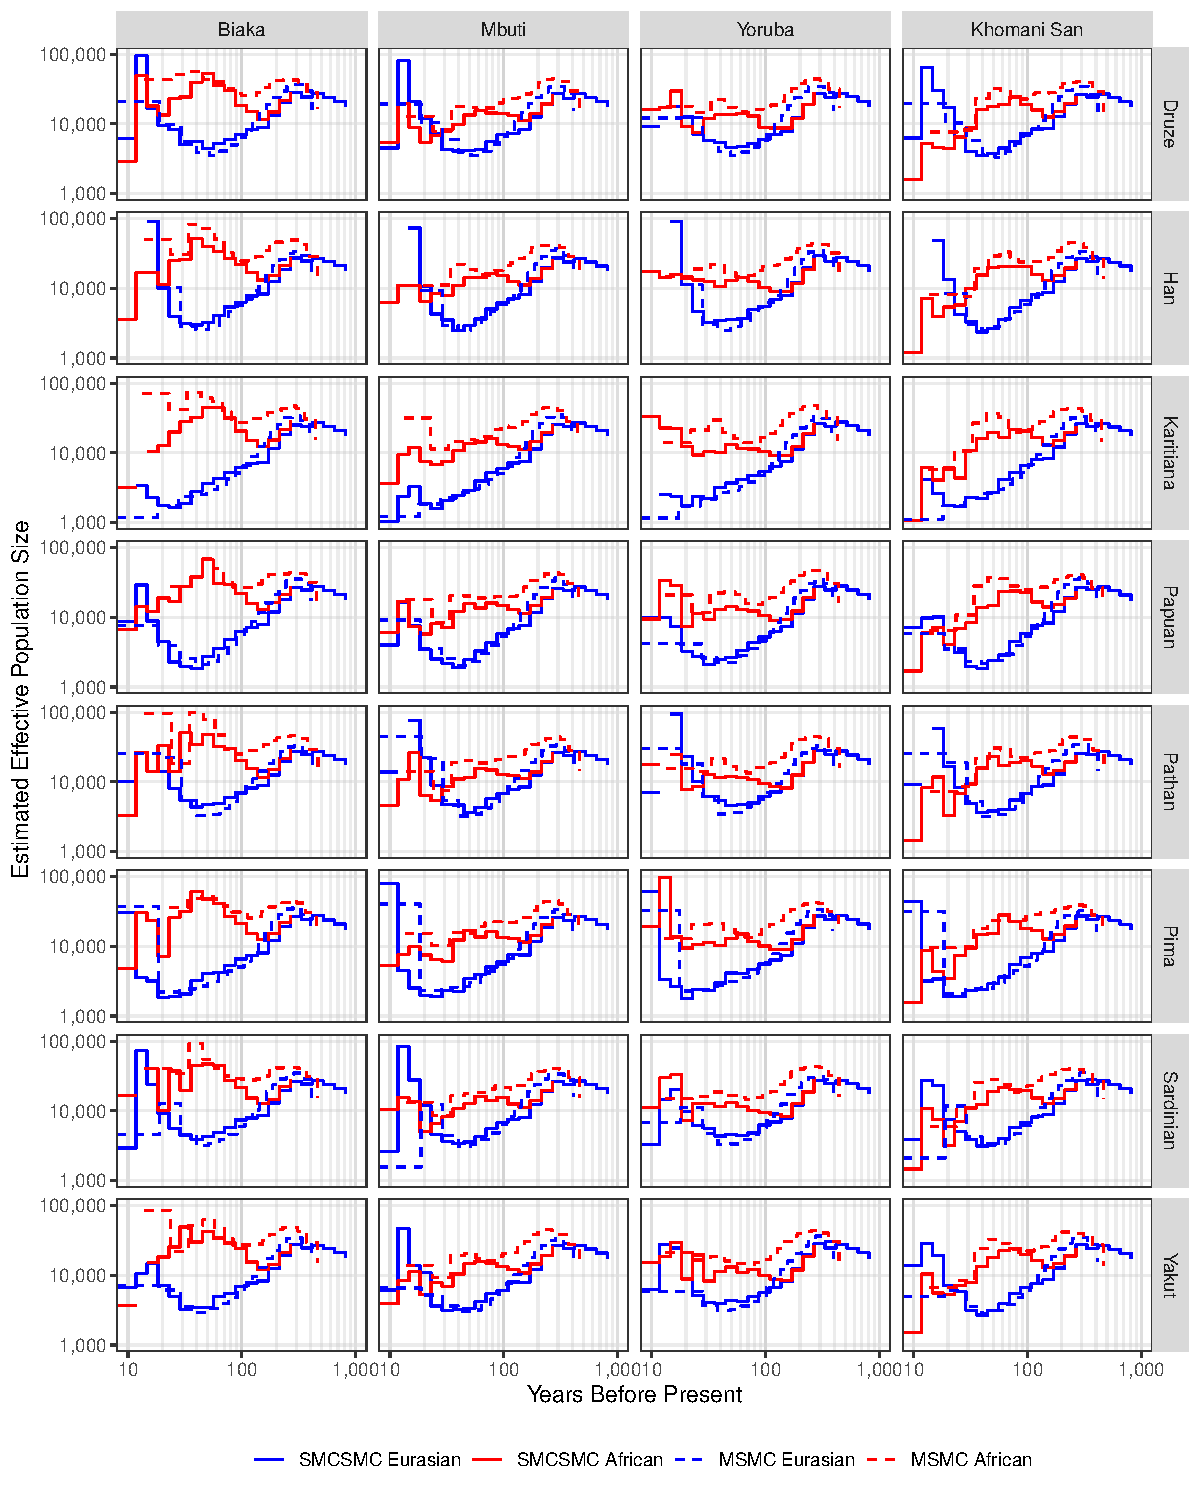
\includegraphics[width=0.9\textwidth]{../plot/sgdp_subet_ne.pdf}
    \caption{{\tt smcsmc} and MSMC inferred effective population size of several populations in the Simons Genome Diversity Panel. These samples were selected to match, as closely as possible, those in the physically phased subet of the Human Genome Diversity Project panel. 10,000 particles and 25 iterations were used for {\tt smcsmc} and 40 iterations for MSMC.}
    \label{hgdp_sgdp_ne}
\end{figure}

\begin{figure}
	\centering
	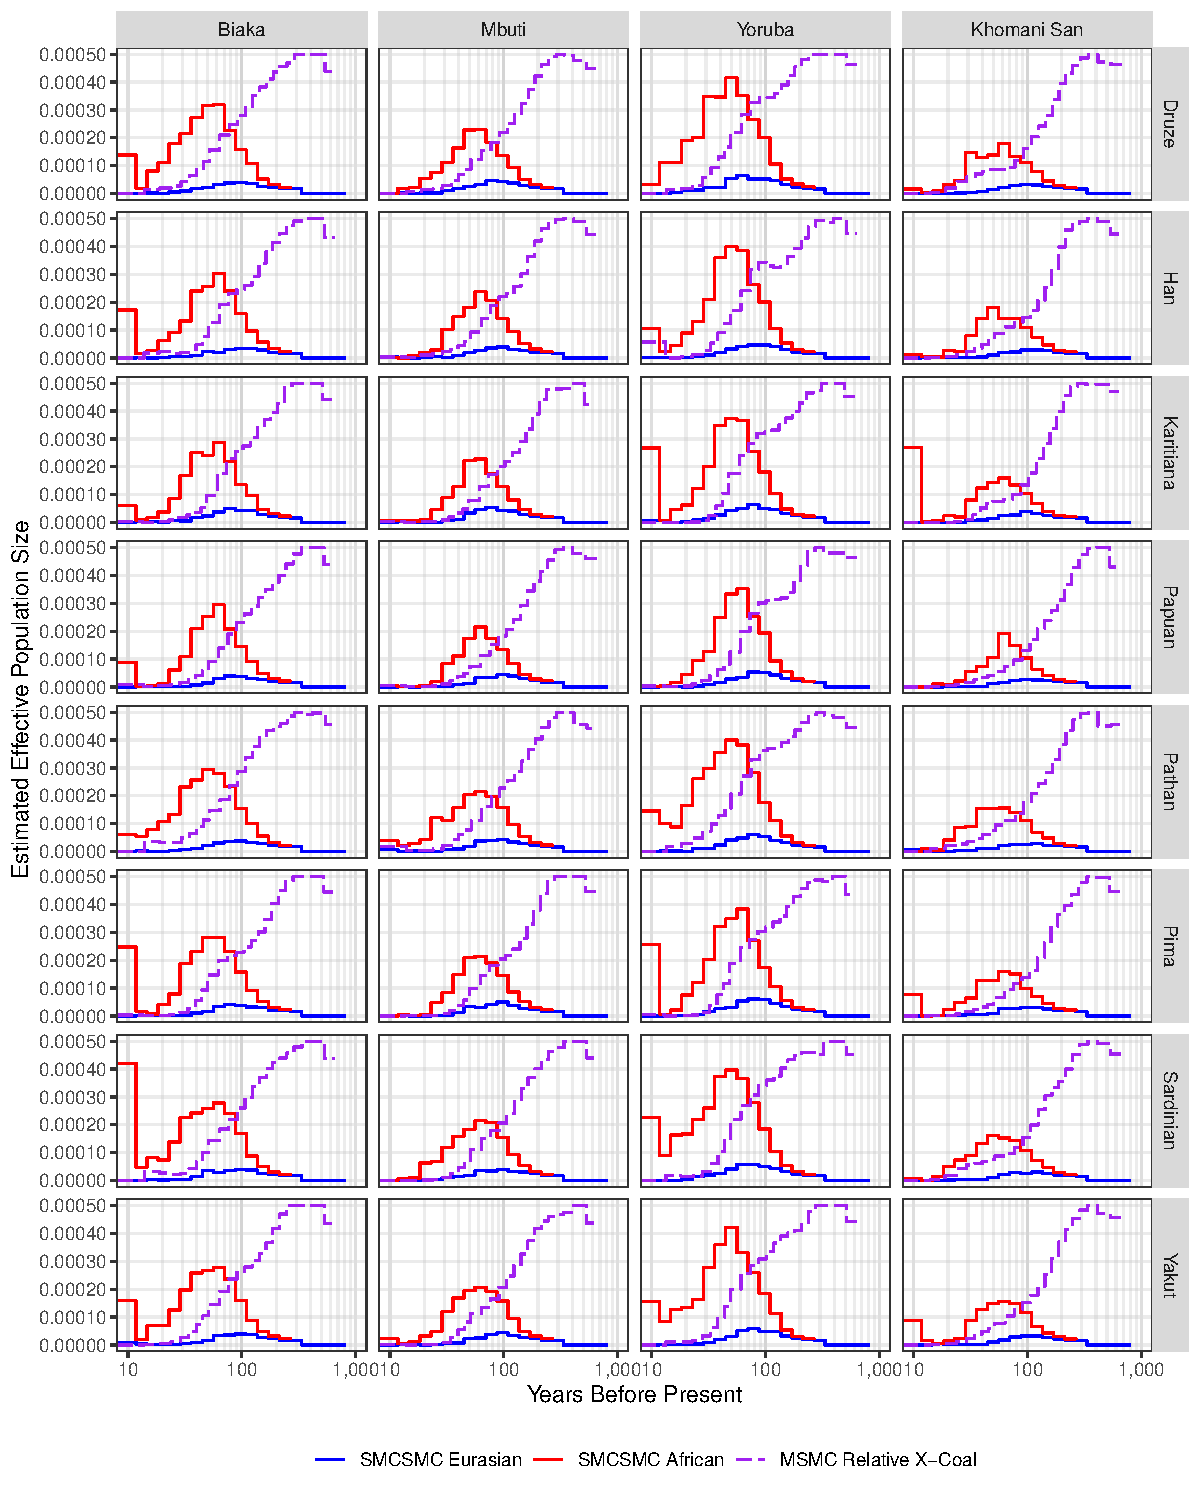
\includegraphics[width=0.9\textwidth]{../plot/sgdp_subet_mig.pdf}
	\caption{Inferred migration using {\tt smcsmc} in the Simons Genome Diversity Panel along with the scaled relative cross-coalescent rate estimated by MSMC. Samples were chosen to match, as closely as possible, those in the physically phased subset of the Human Genome Diversity Project panel. 10,000 particles and 25 iterations were used, 40 in the case for MSMC.}
	\label{fig:hgdp_sgdp_mig}
\end{figure}


\section{Statistical Analysis of Migrated Segments} \label{dstats_section}

\begin{figure}
	\centering
	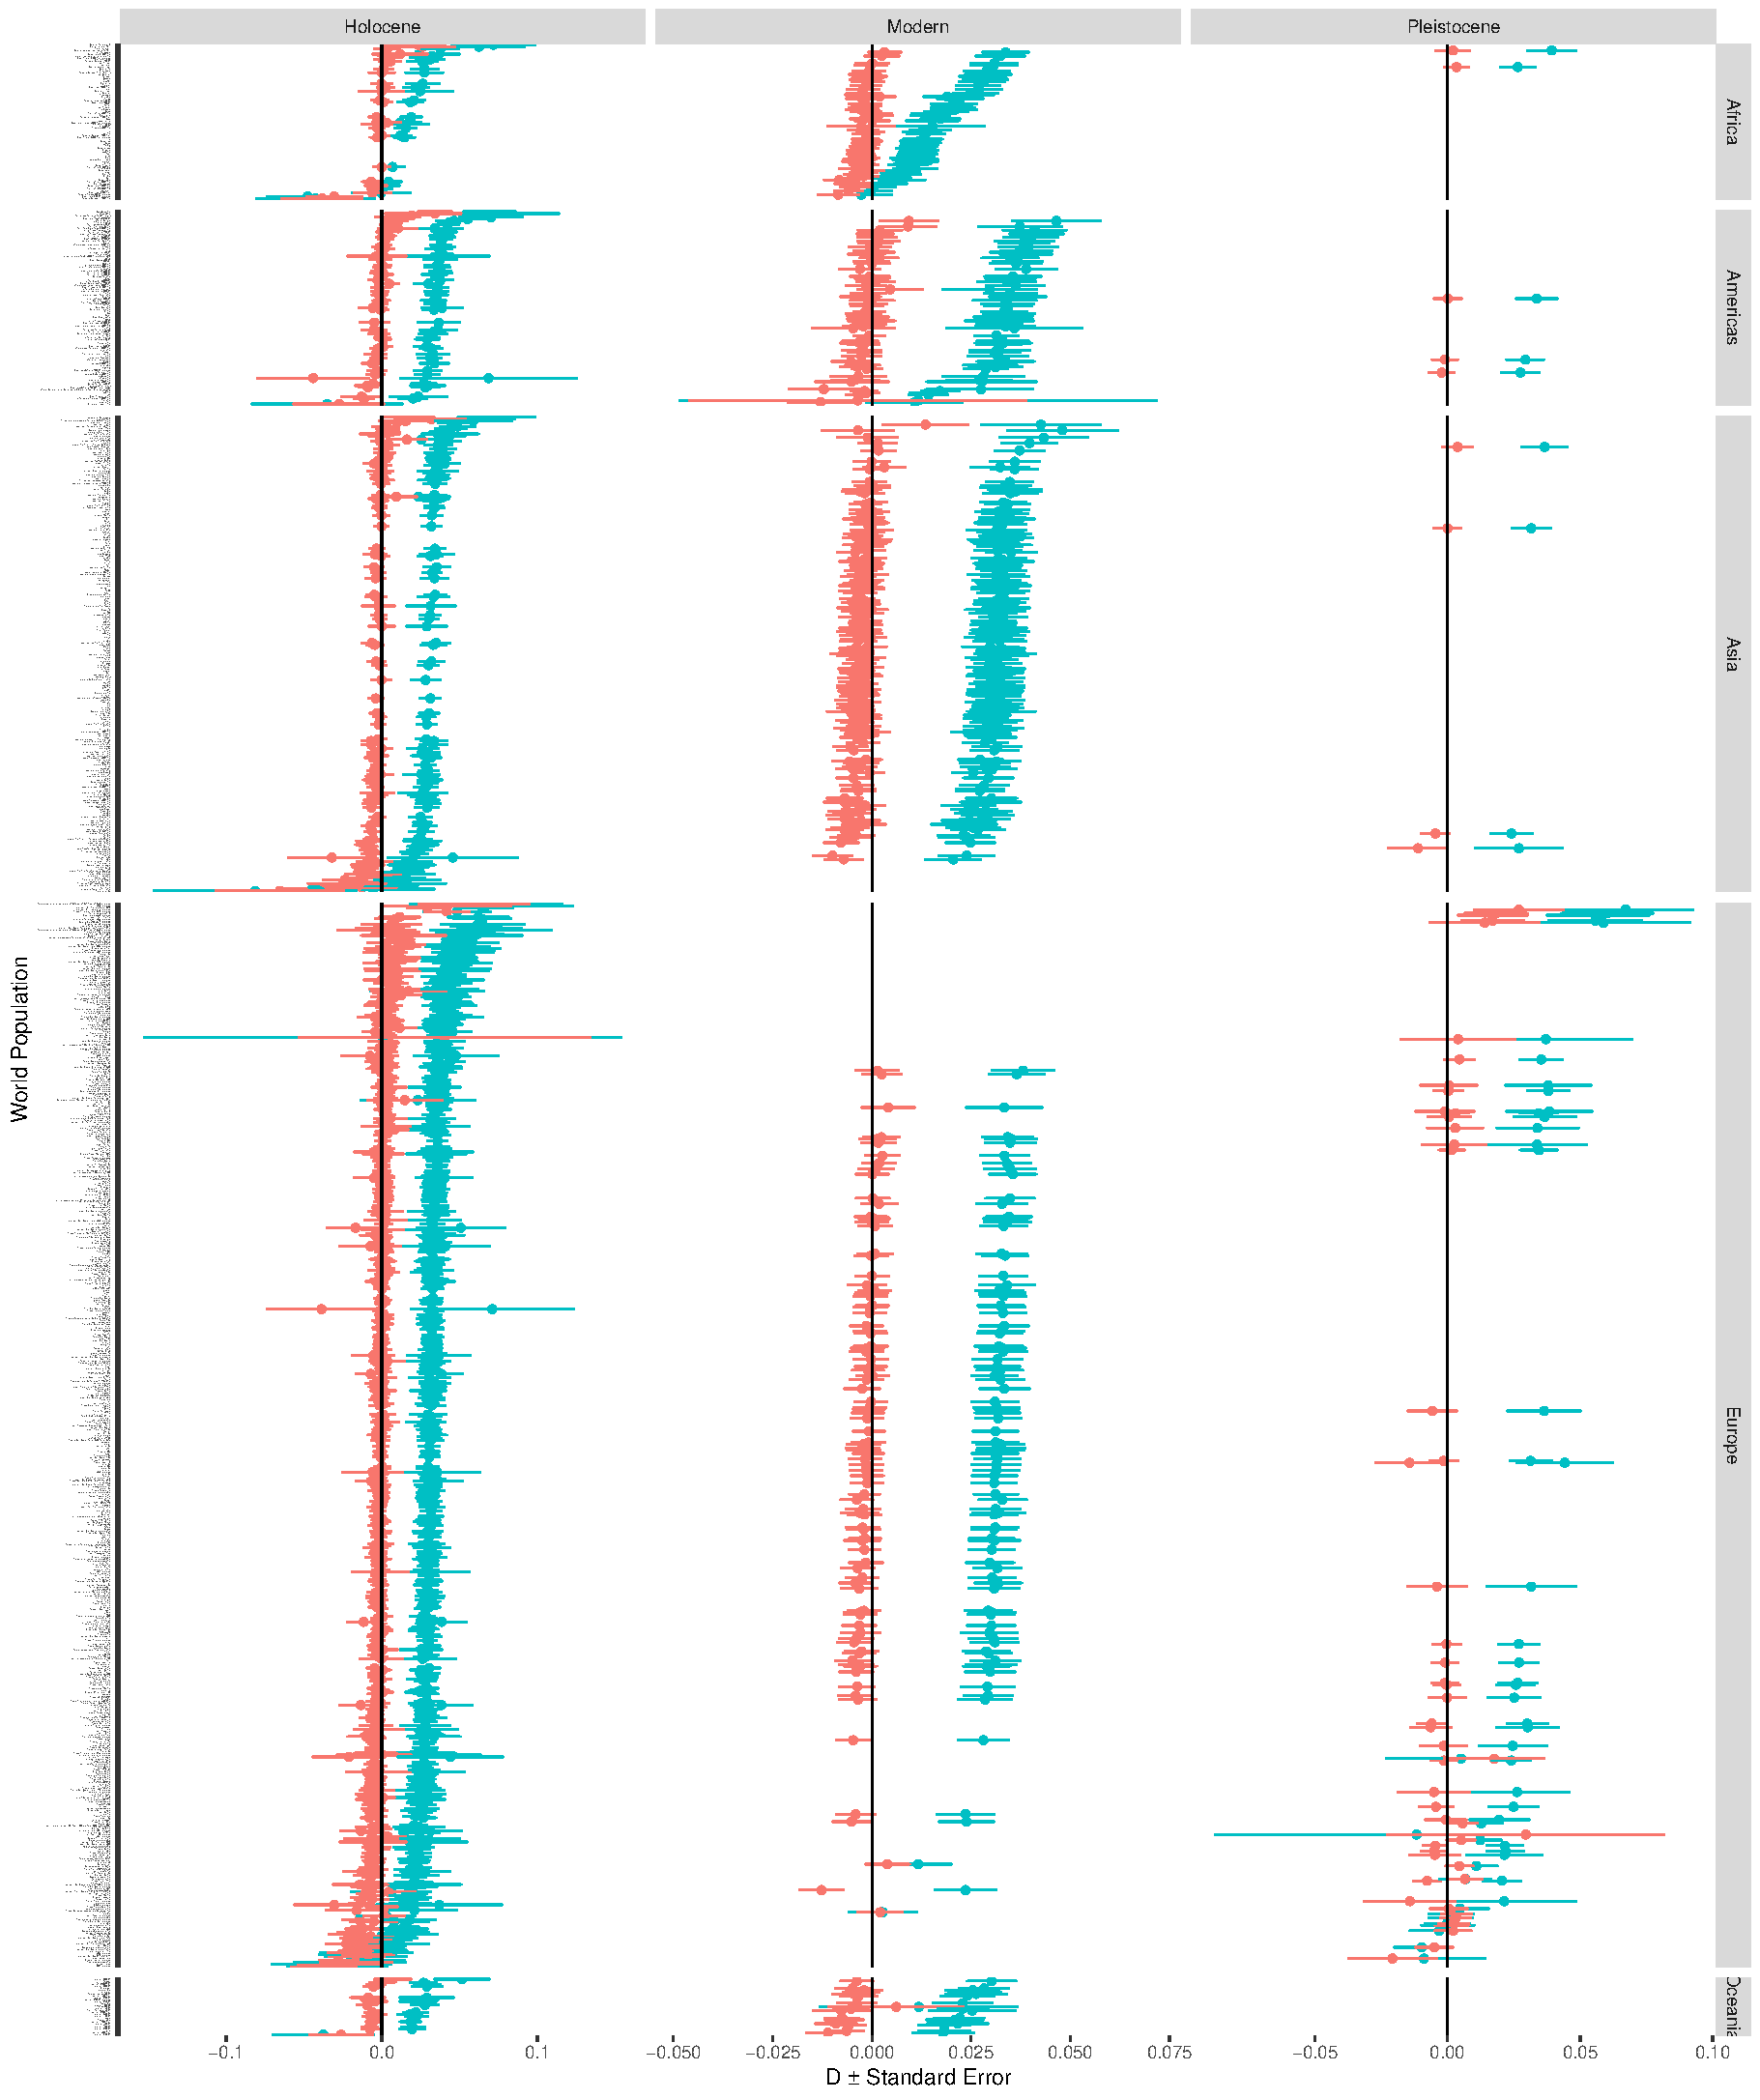
\includegraphics[width=\textwidth]{../plot/yri_d_stats.pdf}
	\caption{D statistics of the form (X, Chimp; Yoruba-1, Yoruba-2) for all global populations in the Human Origins dataset.}
	\label{fig:alld}
\end{figure}


\begin{enumerate}
	\item 
\end{enumerate}

\section{Simulation procedure} \label{simproc}

The ability of {\tt smcsmc} to recover a back-migration signal is evaluated through simulation. One gigabase of sequence was simulated in {\tt scrm}, and subsequently re-inferred by {\tt smcsmc}. Migration is parameterised by three factors, magnitude, midpoint, and duration. A scenario is simulated where the midpoint is the center of a block of a given duration which has uniform migration which integrates to a given total proportion replacement over the period. We use the following demographic model for population size throughout all simulations:

\begin{figure}
    \centering
    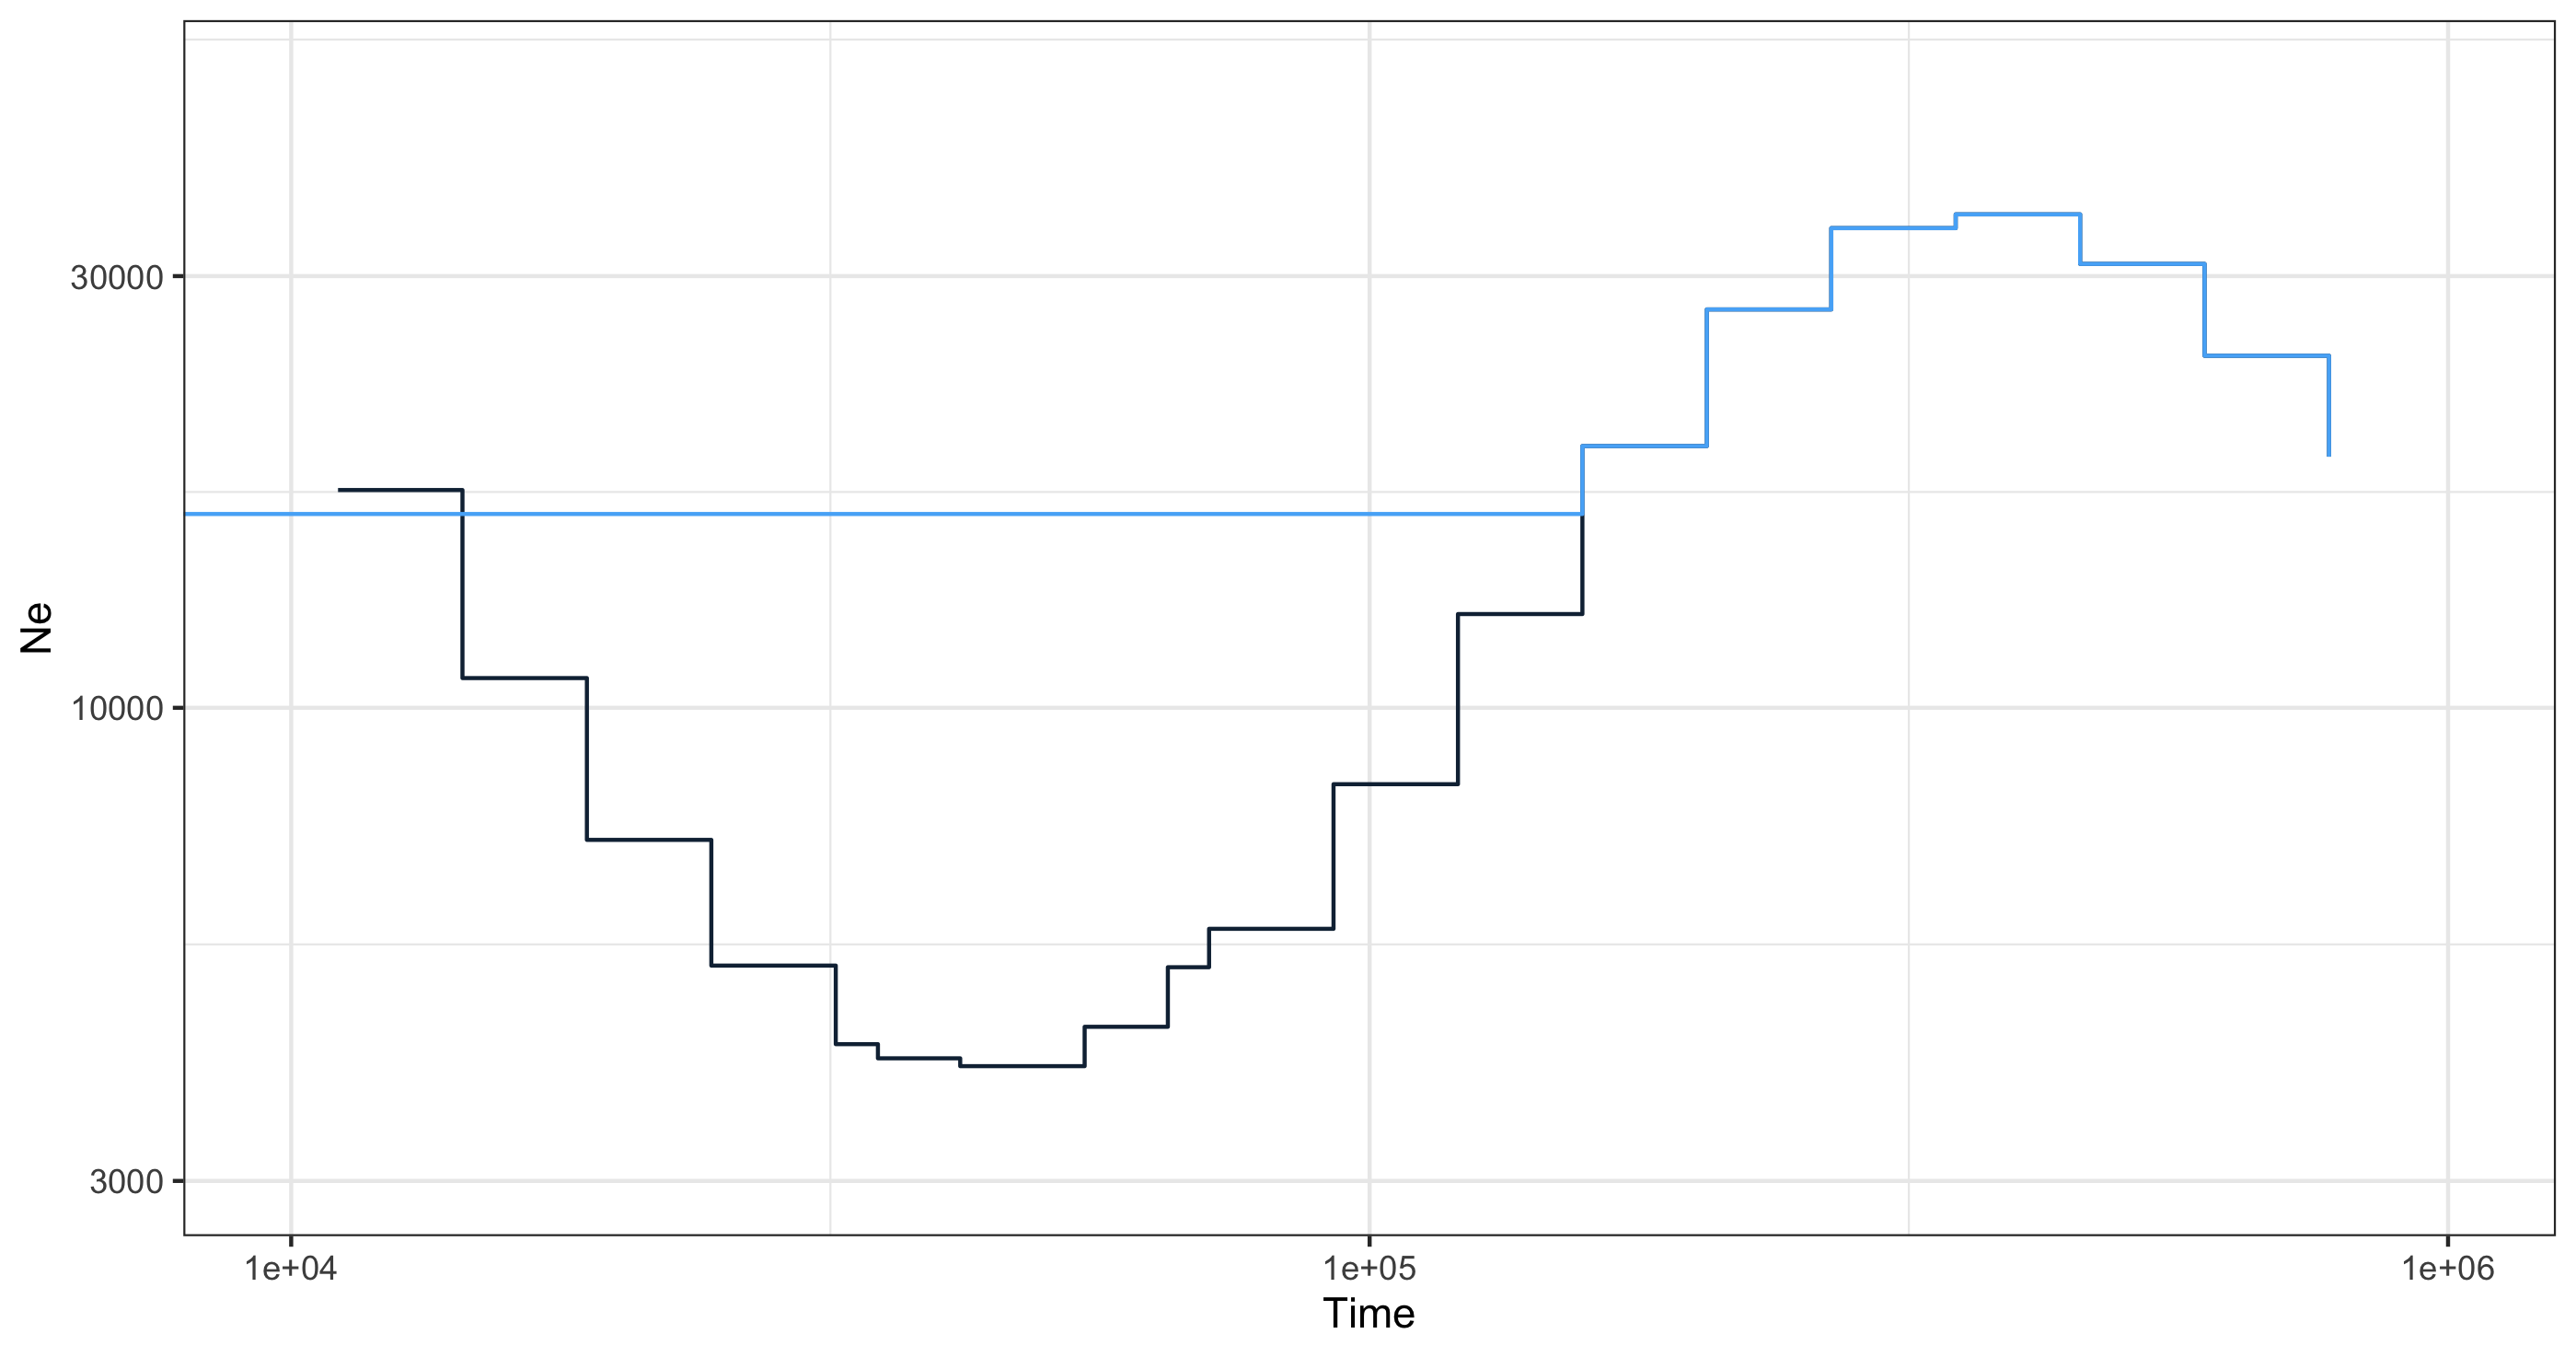
\includegraphics[width = 0.5\linewidth]{../plot/demographic_model.png}
    \caption{Population size model used for simulations.}
    \label{fig:dem}
\end{figure}



The following commands can be used in either {\tt ms} or {\tt SCRM} to specify demographic models. The African population size is given by 

\begin{verbatim}
-en 0.00000000 1 36.9124479 -en 0.00229999 1 14.8978177 -en 0.00299994 1 7.04453213 
-en 0.00391291 1 3.68961222 -en 0.00510371 1 2.06587476 -en 0.00665692 1 1.21617010
-en 0.00868280 1 0.75362392 -en 0.01132521 1 0.49927968 -en 0.01477178 1 0.36258332
-en 0.01926724 1 0.29687253 -en 0.02108190 1 0.28637149 -en 0.02513079 1 0.28071694
-en 0.03277878 1 0.31028768 -en 0.03915210 1 0.36107482 -en 0.04275426 1 0.39815181
-en 0.05576555 1 0.57528787 -en 0.07273654 1 0.88701054 -en 0.09487226 1 1.36014053
-en 0.12374449 1 1.92573639 -en 0.16140334 1 2.36832894 -en 0.21052280 1 2.45284038
-en 0.27459066 1 2.16222564 -en 0.35815613 1 1.71146032 -en 0.46715286 1 1.32388966
-en 0.60932028 1 1.09778746 -en 0.79475315 1 1.04669123 -en 1.03661833 1 1.16969768
-en 1.35208972 1 1.45788656 -en 1.76356769 1 1.80077313 -en 2.30026970 1 1.89942369
\end{verbatim}

While the European population size is given by

\begin{verbatim}
-en 0.00000000 2 1.14422216 -en 0.00229999 2 1.14422216 -en 0.00299994 2 1.14422216
-en 0.00391291 2 1.14422216 -en 0.00510371 2 1.14422216 -en 0.00665692 2 1.14422216
-en 0.00868280 2 1.14422216 -en 0.01132521 2 1.14422216 -en 0.01477178 2 1.14422216
-en 0.01926724 2 1.14422216 -en 0.02108190 2 1.14422216 -en 0.02513079 2 1.14422216
-en 0.03277878 2 1.14422216 -en 0.03915210 2 1.14422216 -en 0.04275426 2 1.14422216
-en 0.05576555 2 1.14422216 -en 0.07273654 2 1.14422216 -en 0.09487226 2 1.36014053
-en 0.12374449 2 1.92573639 -en 0.16140334 2 2.36832894 -en 0.21052280 2 2.45284038 
-en 0.27459066 2 2.16222564 -en 0.35815613 2 1.71146032 -en 0.46715286 2 1.32388966
-en 0.60932028 2 1.09778746 -en 0.79475315 2 1.04669123 -en 1.03661833 2 1.16969768
-en 1.35208972 2 1.45788656 -en 1.76356769 2 1.80077313 -en 2.30026970 2 1.89942369
\end{verbatim}

Times are in units of $4gN_0$ while population sizes are in units of $N_0$. For $g=29, N_0 = 14312$, the demographic model is as shown in Supplemental Figure \ref{fig:dem}.  

The demographic model which we have assumed for both population's effective sizes has been shown to recapitulate similar inference to real data (data not shown). The migration parameter must be initiated at a given magnitude; further back in time, the particle filter is less able to identify lineage's true populations, and the inference of migration rates becomes essential uniform. Thus, we see a ``drop-off'' effect, where in the ancient past, the inference remains at the initiation value, and as more certainty about different histories is obtained, the migration values recapitulate real information. Thus the choice of an appropriate parameter for the initial migration rate is a crucial step in {\tt smcsmc} analysis, and here we chose to arrive at this value through simulation.

We simulate back-migration scenarios of varying total migration proportions from 0 (no migration) up to 60\% population replacement.For each simulation, we initiate the particle filter at either 0, 1, or 5 4$N_0$ proportion replaced per generation (which are the units used internally by {\tt scrm} and {\tt ms} for simulation).  {\tt smcsmc} is then used to infer effective population size and migration histories in five iterations with 5000 particles. As a cautionary note, these simulations are almost certainly not fully converged, and are used as an indication of power. Their power, theoretically, approaches 1, as particle filters asymptotically exactly approach the true posterior distribution. However, these low resolution attempts are indicative of a ``quick'' overview of the abilities of the algorithm. With 600 cores available, each of the cases (forward, backward, or bidirectional) was able to run in approximately 20 hours. 

Generally, beginning with a higher migration rate seems to recover a higher proportion of the simulated migration. However, as in the case of a 60\% replacement simulated 40kya, beginning with 5 4$N_0$ rather than 1 4$N_0$ recovers similar proportions of backwards migration (0.502 vs 0.52) yet the higher migration rate finds 0.301 Eurasian migration rather than 0.195. The higher initial migration rates thus slightly reduce power (though, not in all cases, and for fully converged solutions, we would expect both proportions to be similar up to noise) while additionally finding an increased migration in the opposite direction.  Beginning with a zero rate leads to highly unstable estimates of the migration rate and effective population size, and we exclude it from our analysis.

We select a more comprehensive set of initiation parameters and particle values and use them to analyze a Yoruban and French individual from SGDP (Fig \ref{init_yri}). The effect of the initial migration rate seems relatively consistent for low values (0.5 - 2.0),while an increasingly small migration peak is seen for higher initial magnitudes 4.0 - 10.0. Again, beginning with an initial rate of zero tends to lead to highly unstable estimates of effective population size and migration rates. For the remainder of the analyses in this article, we choose to use an initial rate of 1.0. 


\begin{figure}
	\centering
	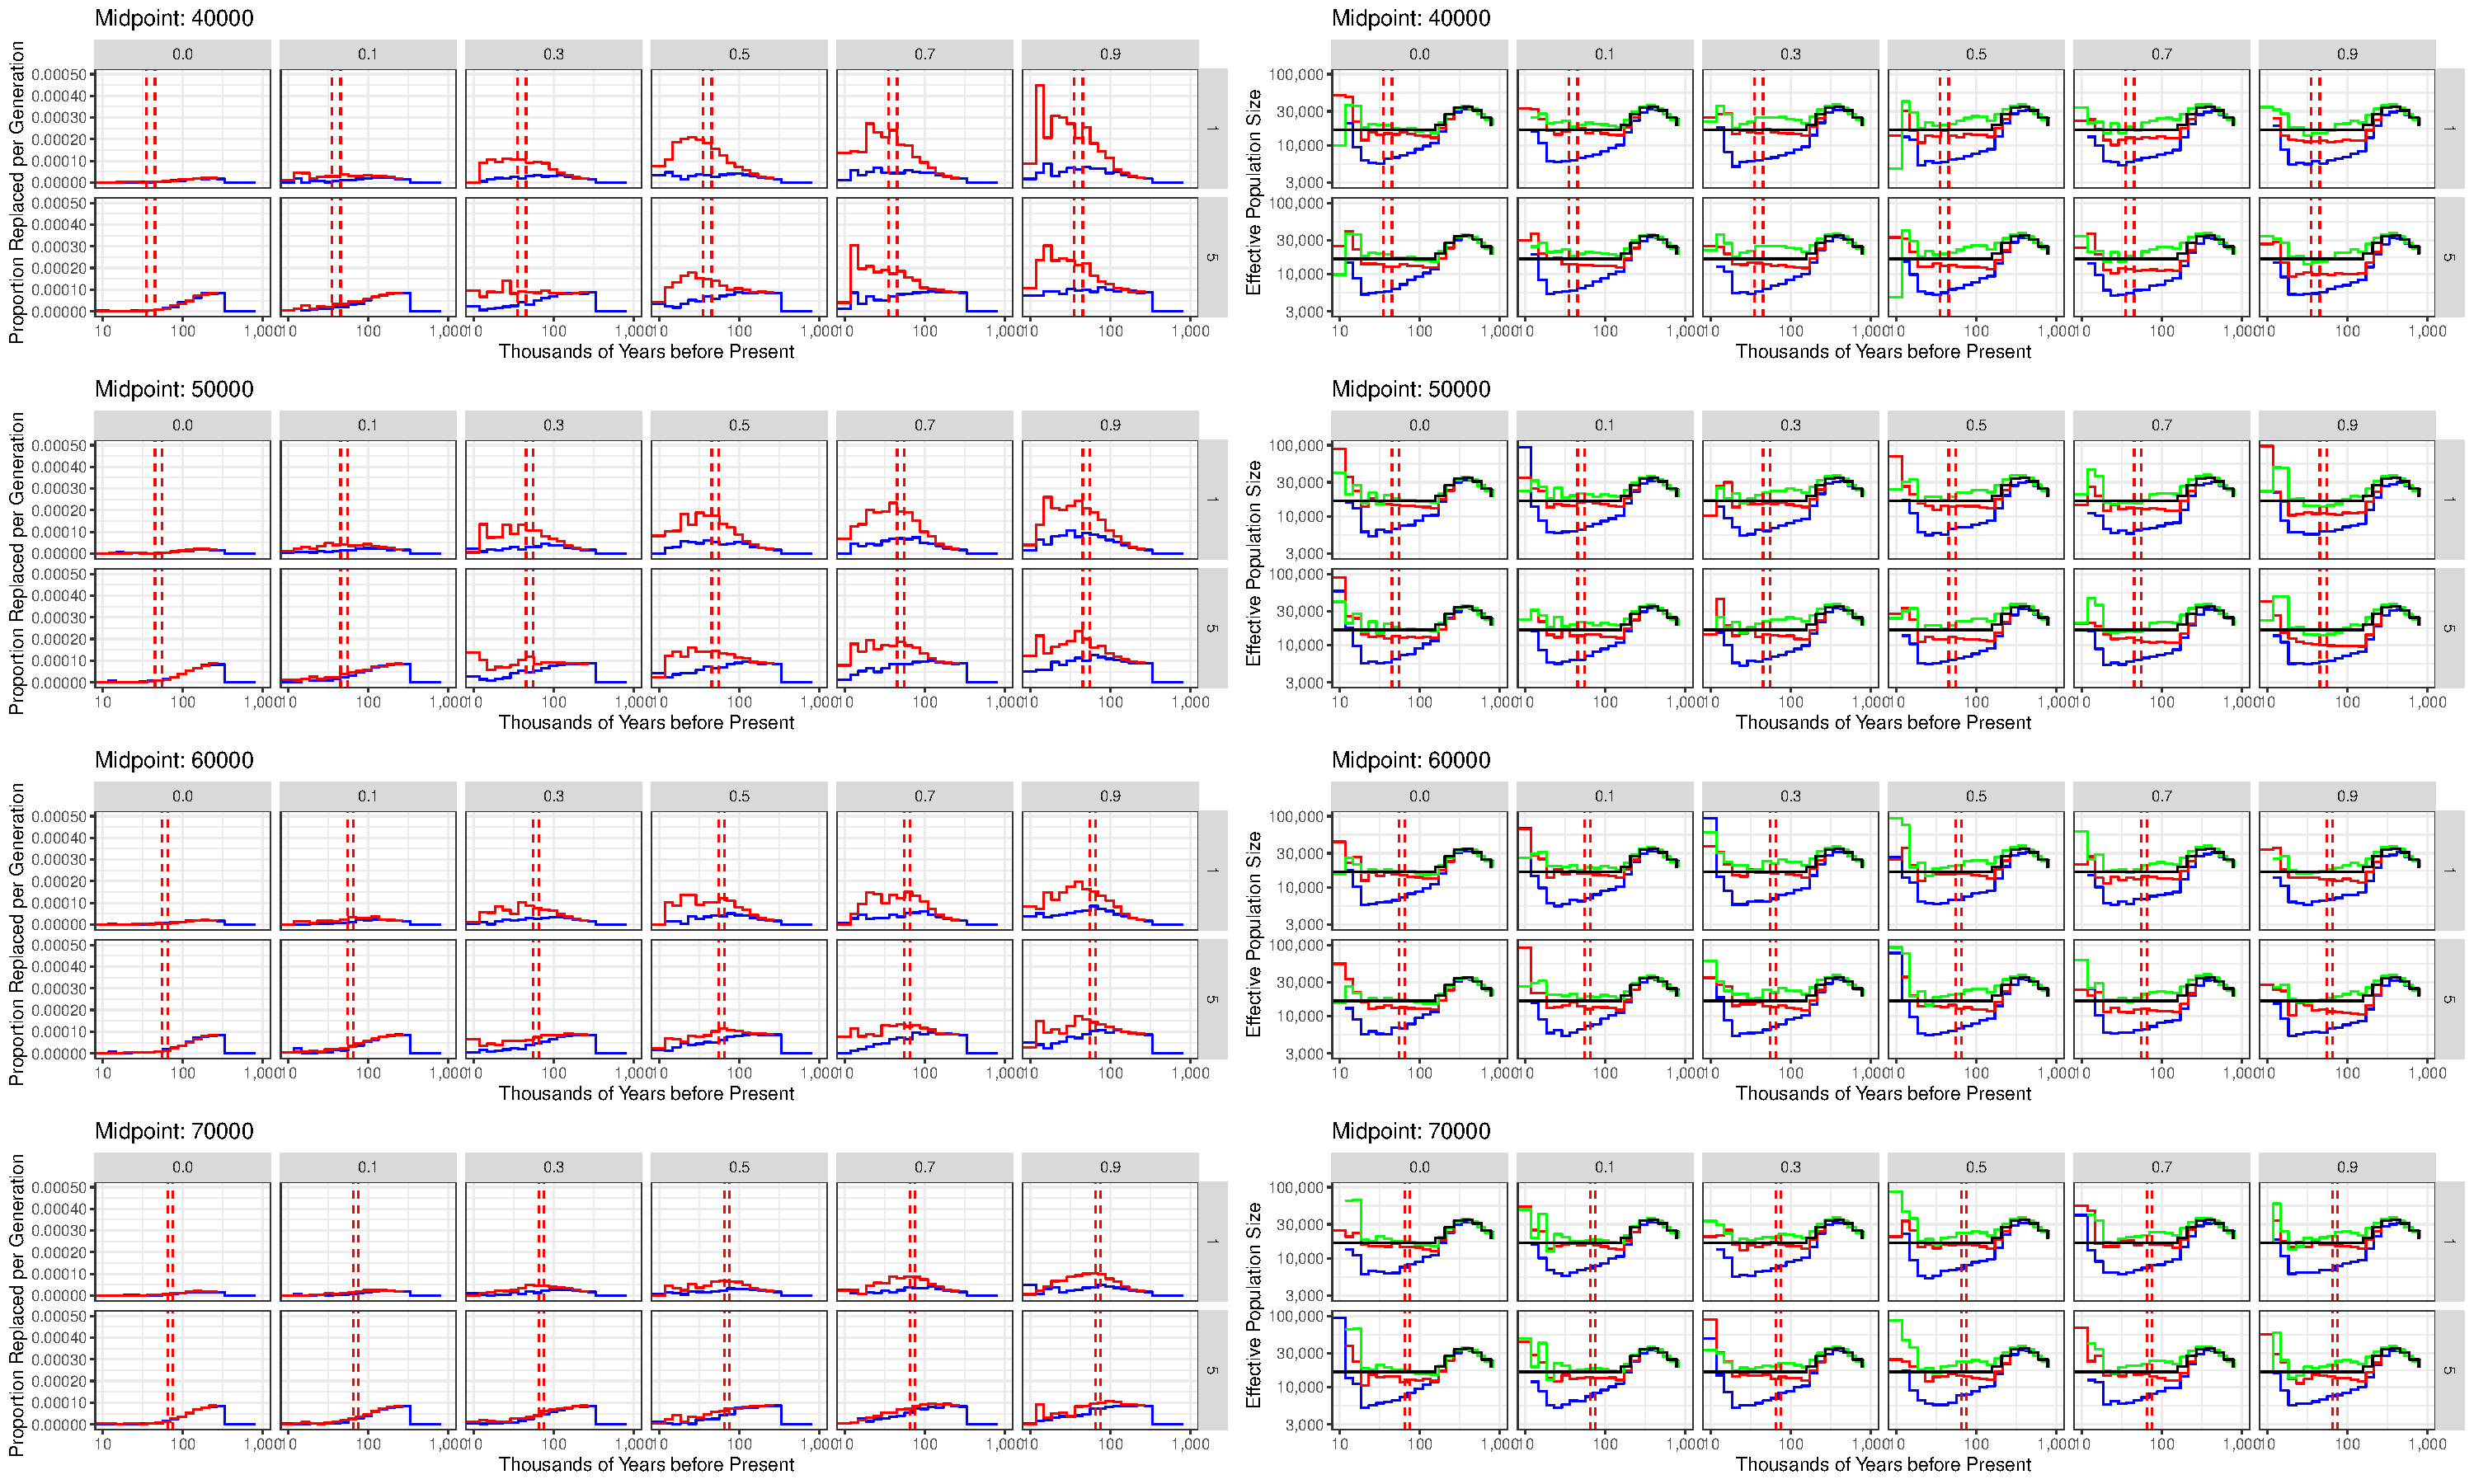
\includegraphics[width=\textwidth]{../plot/sims/backward_different_starts.pdf}
	\caption{Backwards simulation}
	\label{fig:backsim}
\end{figure}


\begin{figure}
	\centering
	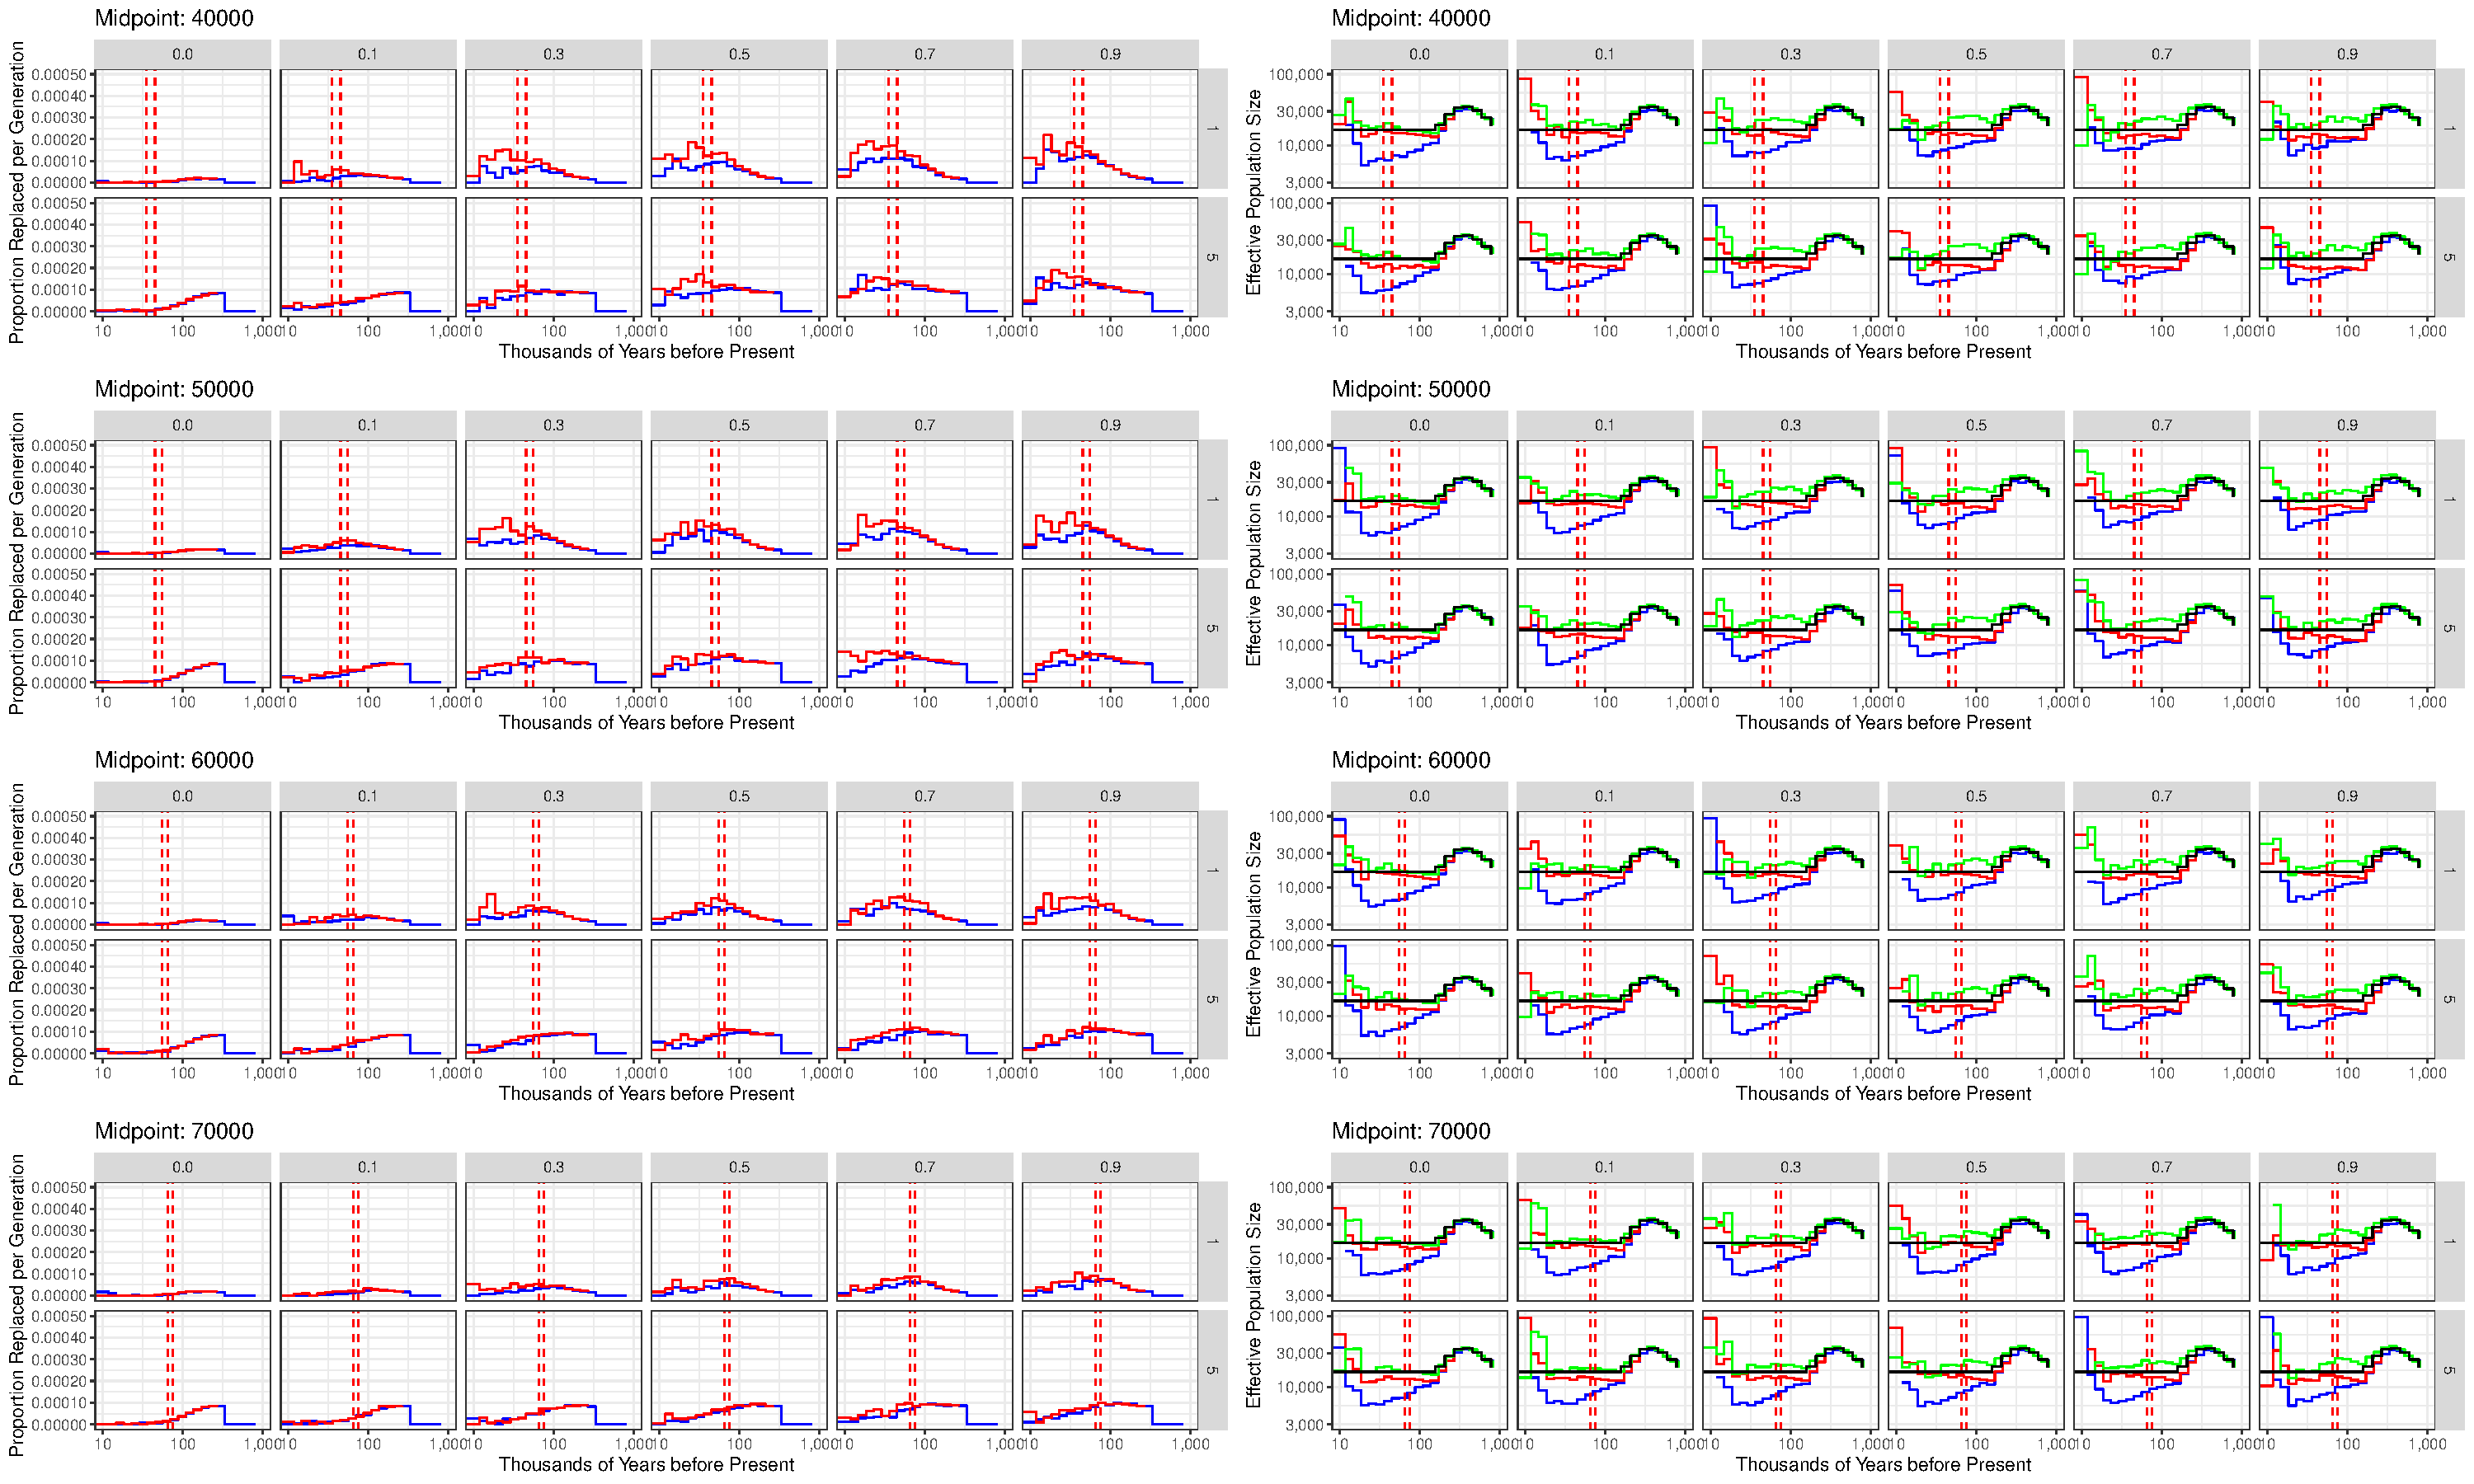
\includegraphics[width=\textwidth]{../plot/sims/bidirectional_different_starts.pdf}
	\caption{Bidirectional simulation}
	\label{fig:bisim}
\end{figure}

\begin{figure}
	\centering
	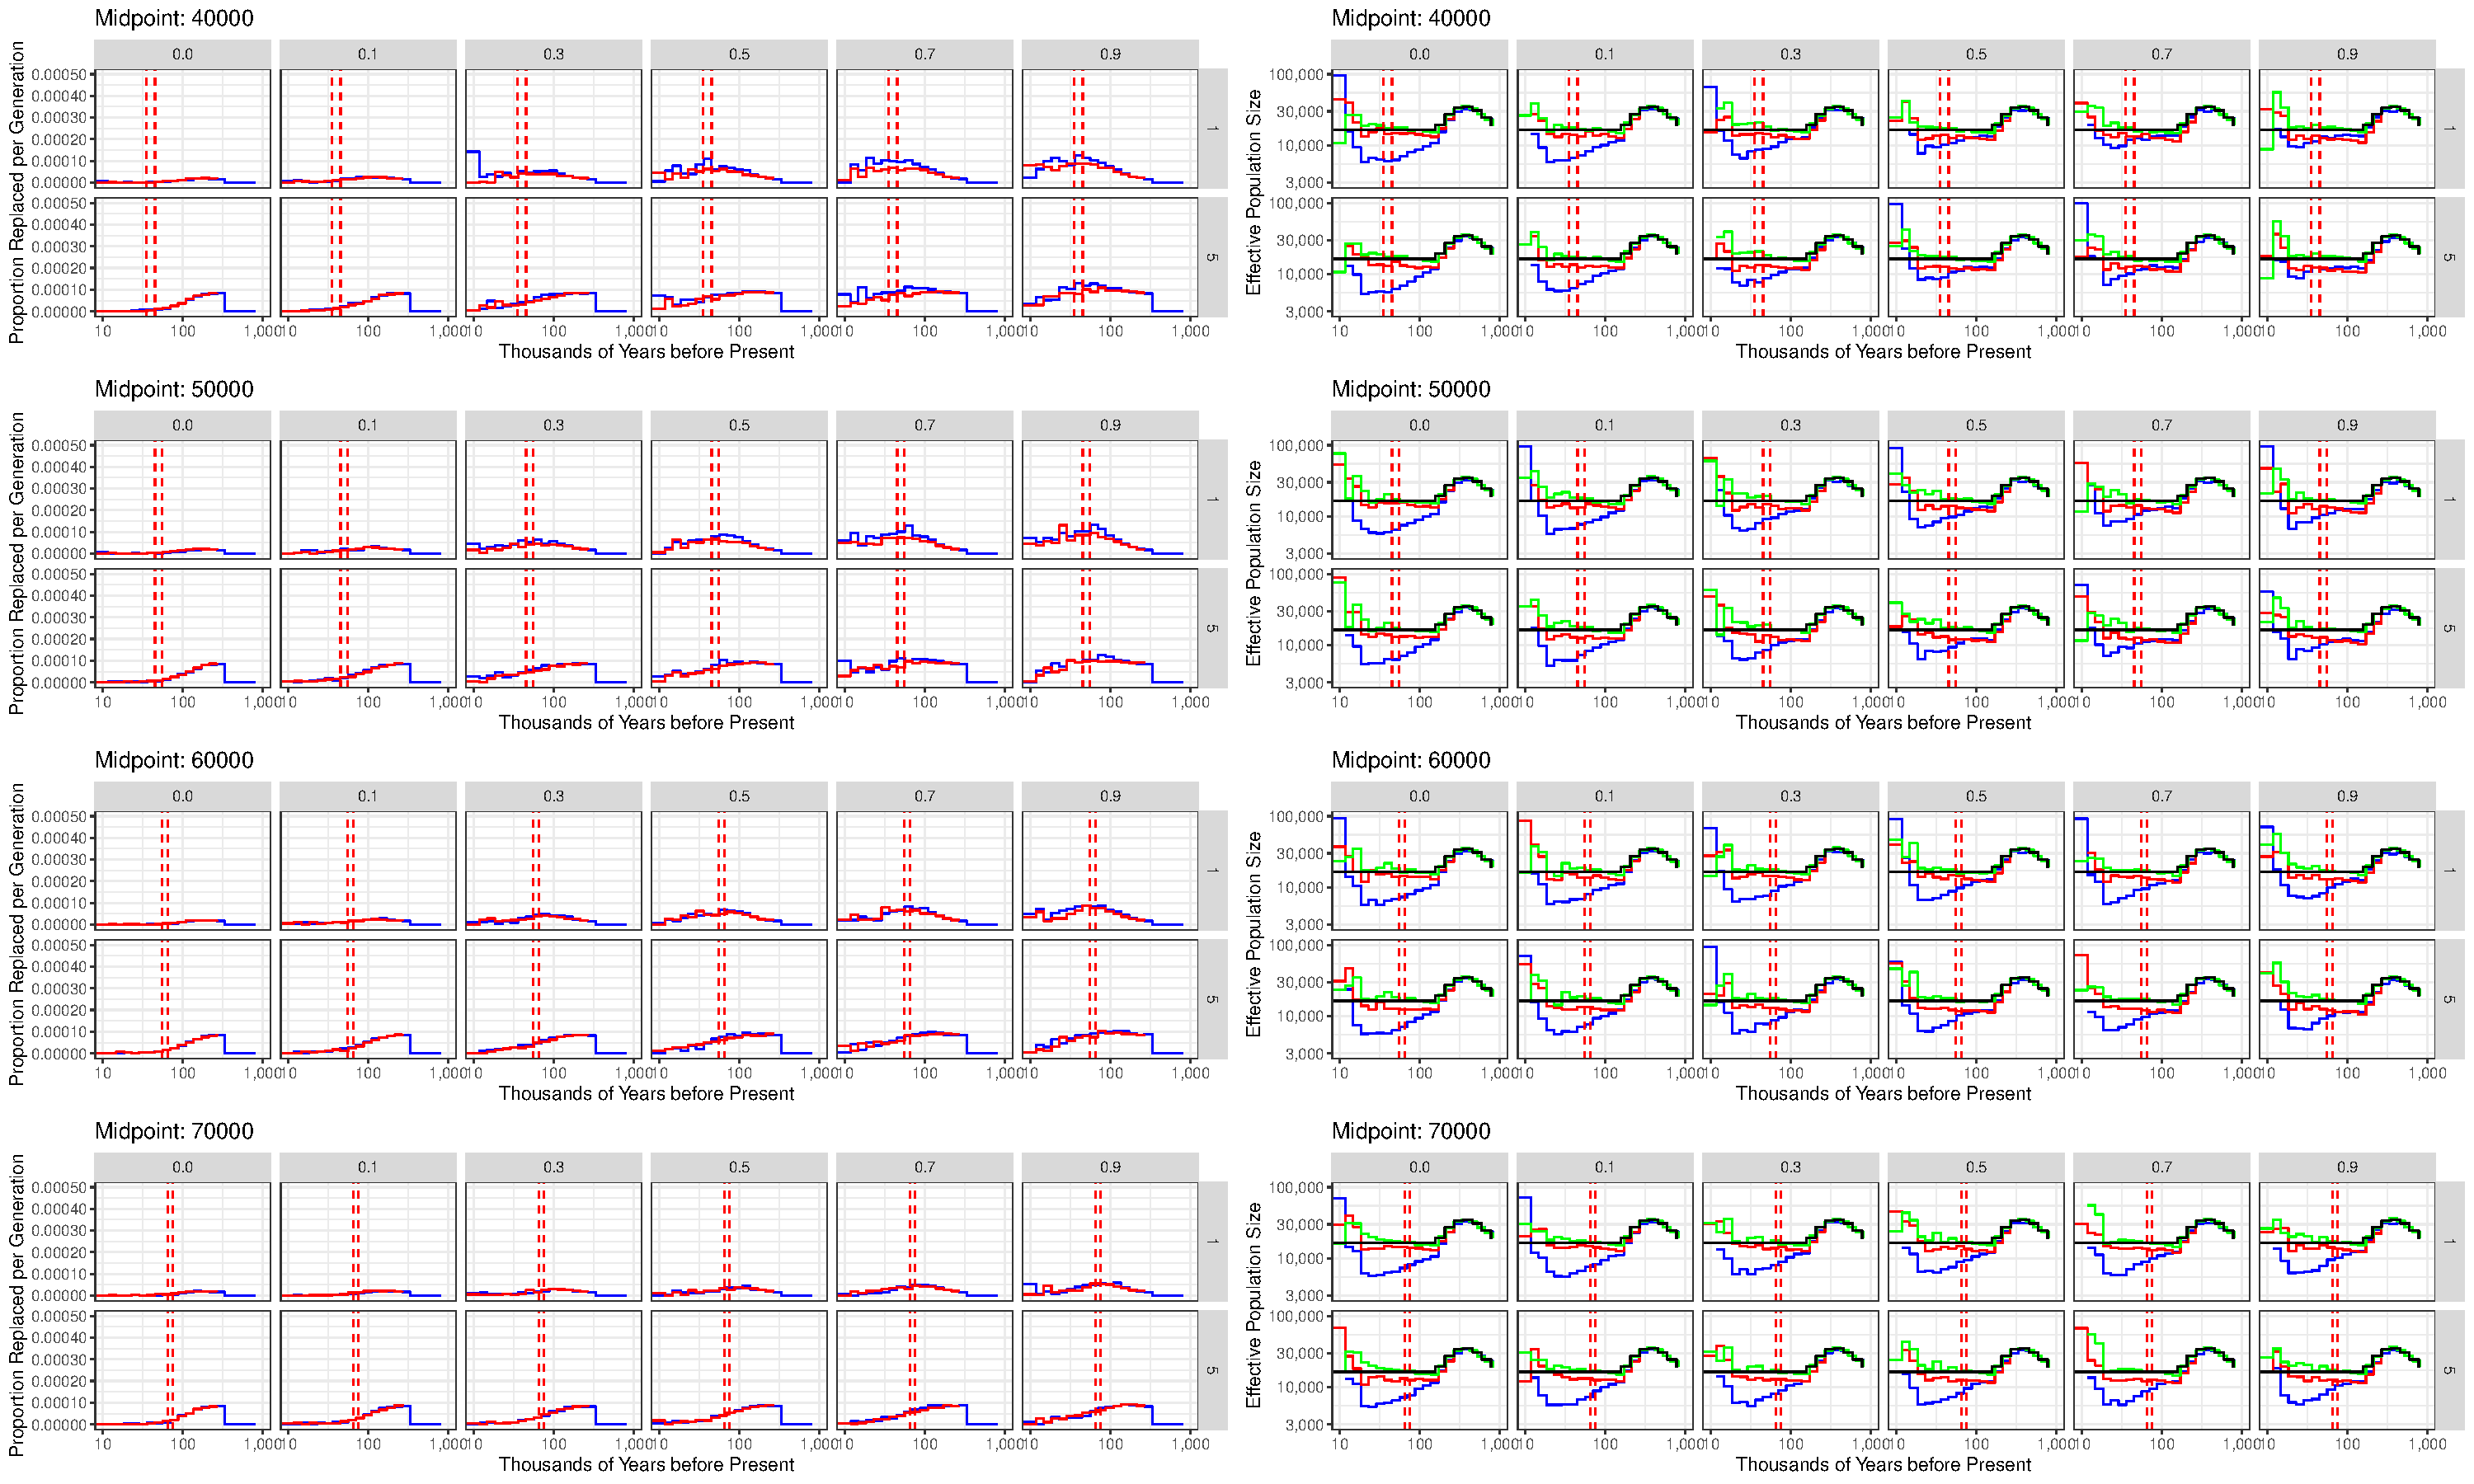
\includegraphics[width=\textwidth]{../plot/sims/forward_different_starts.pdf}
	\caption{Forward simulation}
	\label{fig:fwdsim}
\end{figure}


\begin{figure}
	\centering
	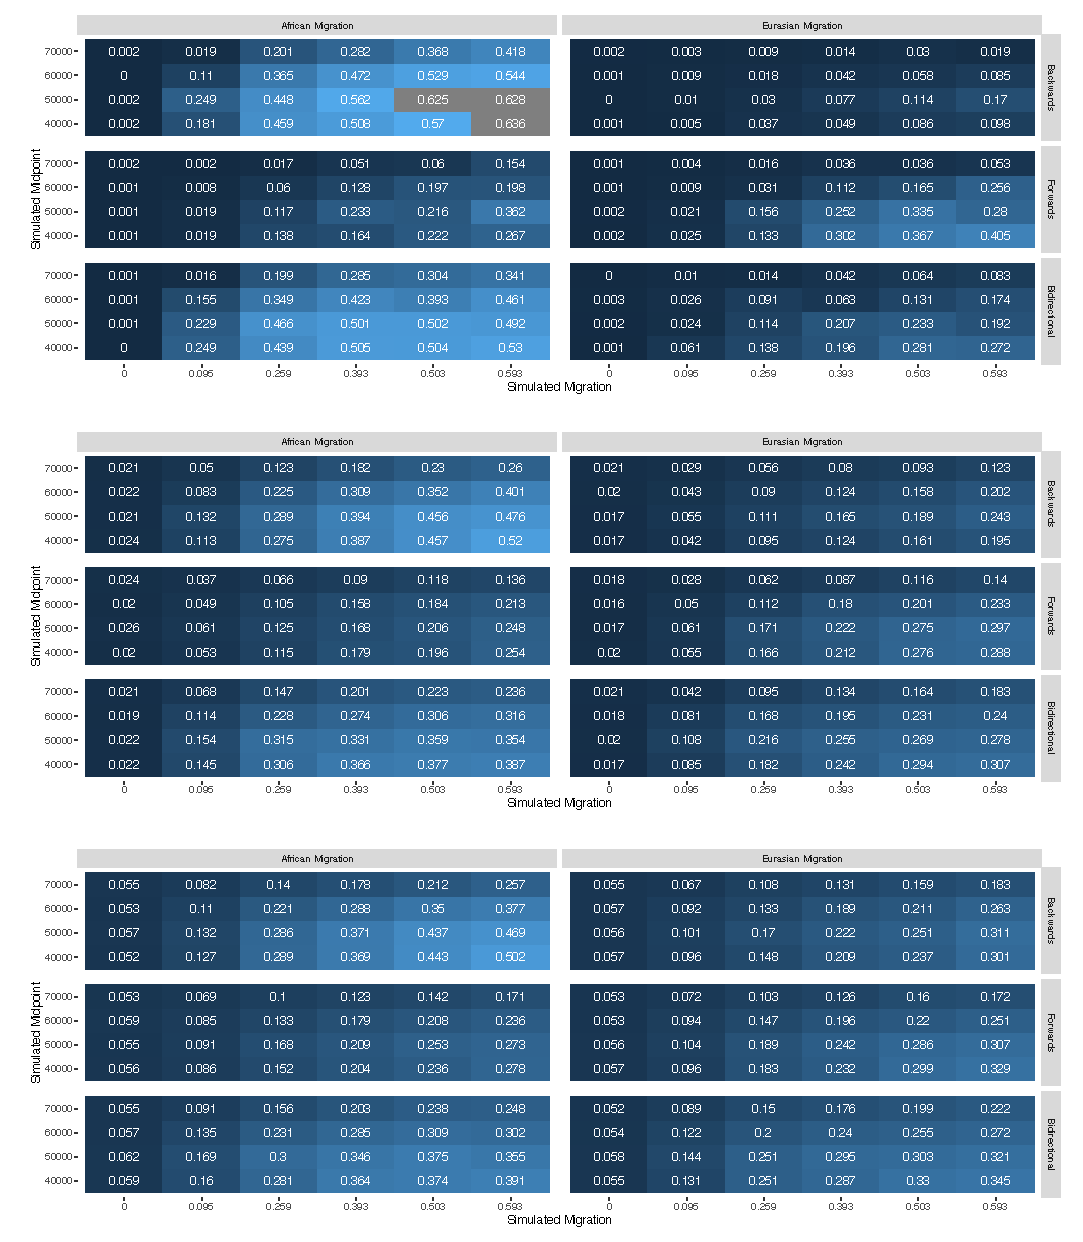
\includegraphics[width=\textwidth]{../plot/sims/all_integrated_sims.pdf}
	\caption{Area under the migration curve for three cases of simulated demography shown in Figures \ref{fig:backsim}, \ref{fig:bisim}, and \ref{fig:fwdsim}. From top to bottom, inference was initiated with 0, 1, and 5 4$N_0$ population replacement per generation.}
	\label{fig:intsim}
\end{figure}


%\begin{figure}
%	\centering
%	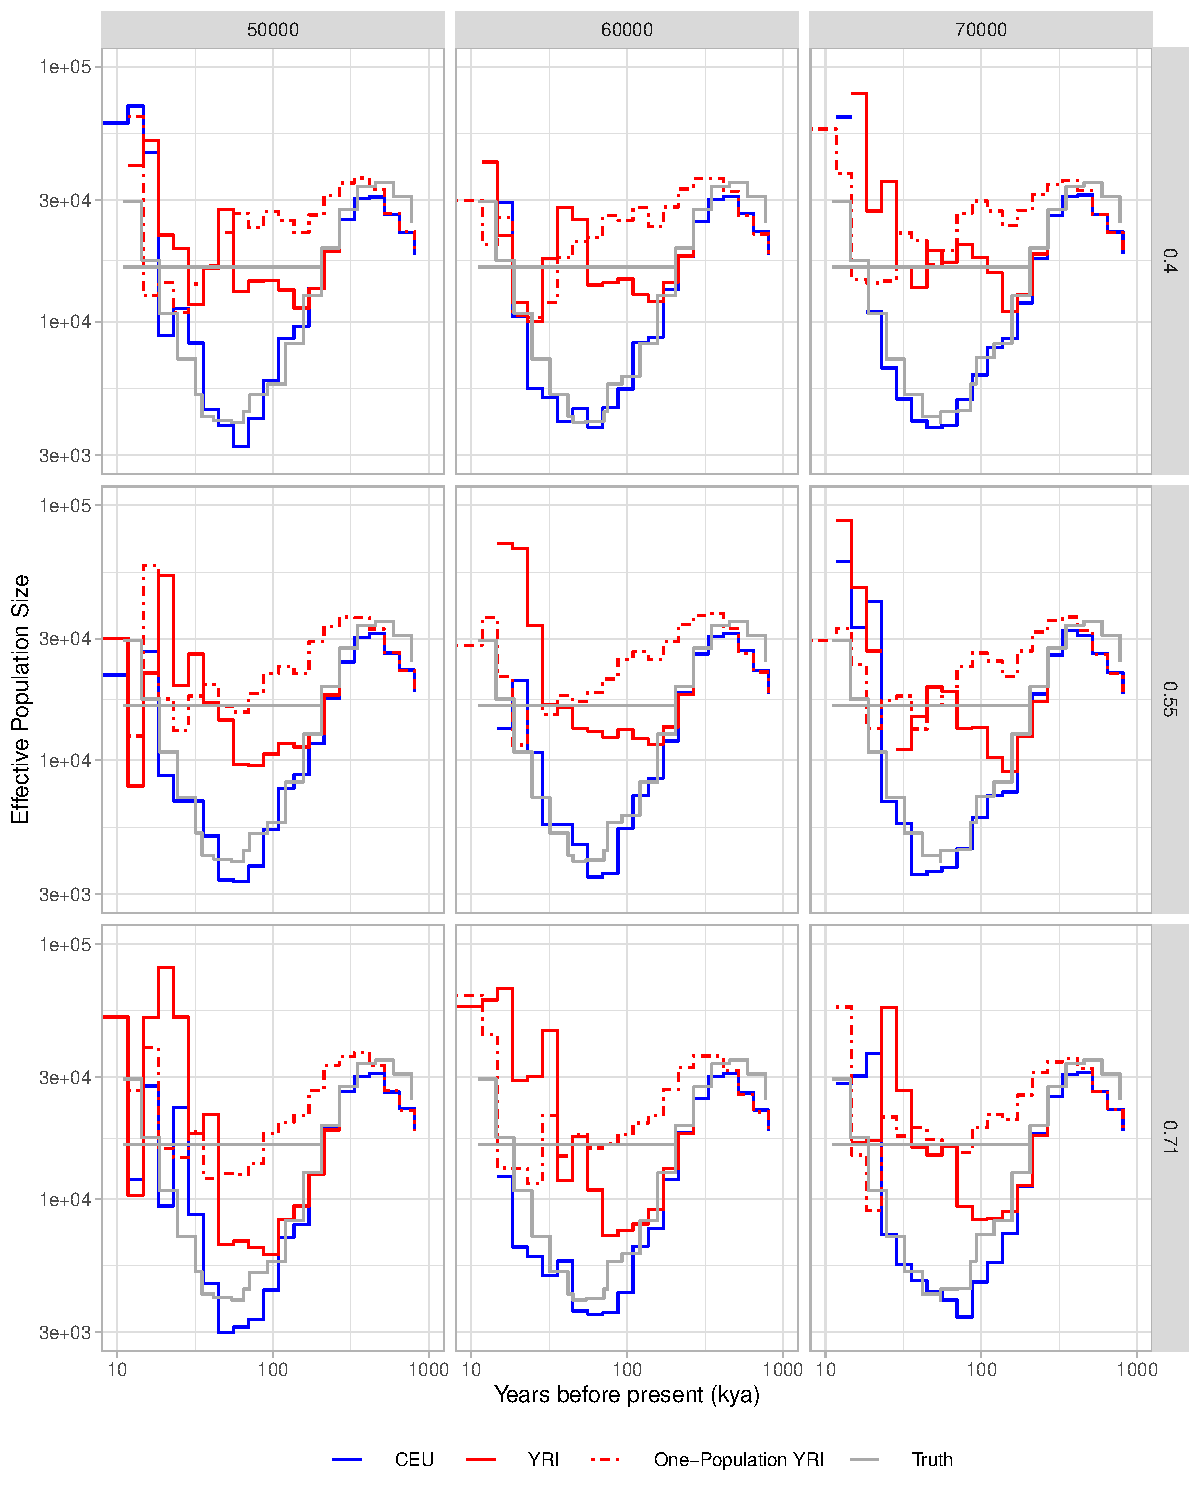
\includegraphics[width=0.5\textwidth]{../plot/old_all_li_durbin.pdf}
%	\caption{Simulated directional migration from effective ``African'' to ``Eurasian'' populations. For this figure, duration of the migration was fixed at 10ky. Simulations performed in {\tt scrm} with one gigabase of sequence. Inference performed in {\tt smcsmc} with five iterations of variational Bayes and 5000 particles.}
%	\label{nesims_10ky}
%\end{figure}

\begin{figure}
	\centering
	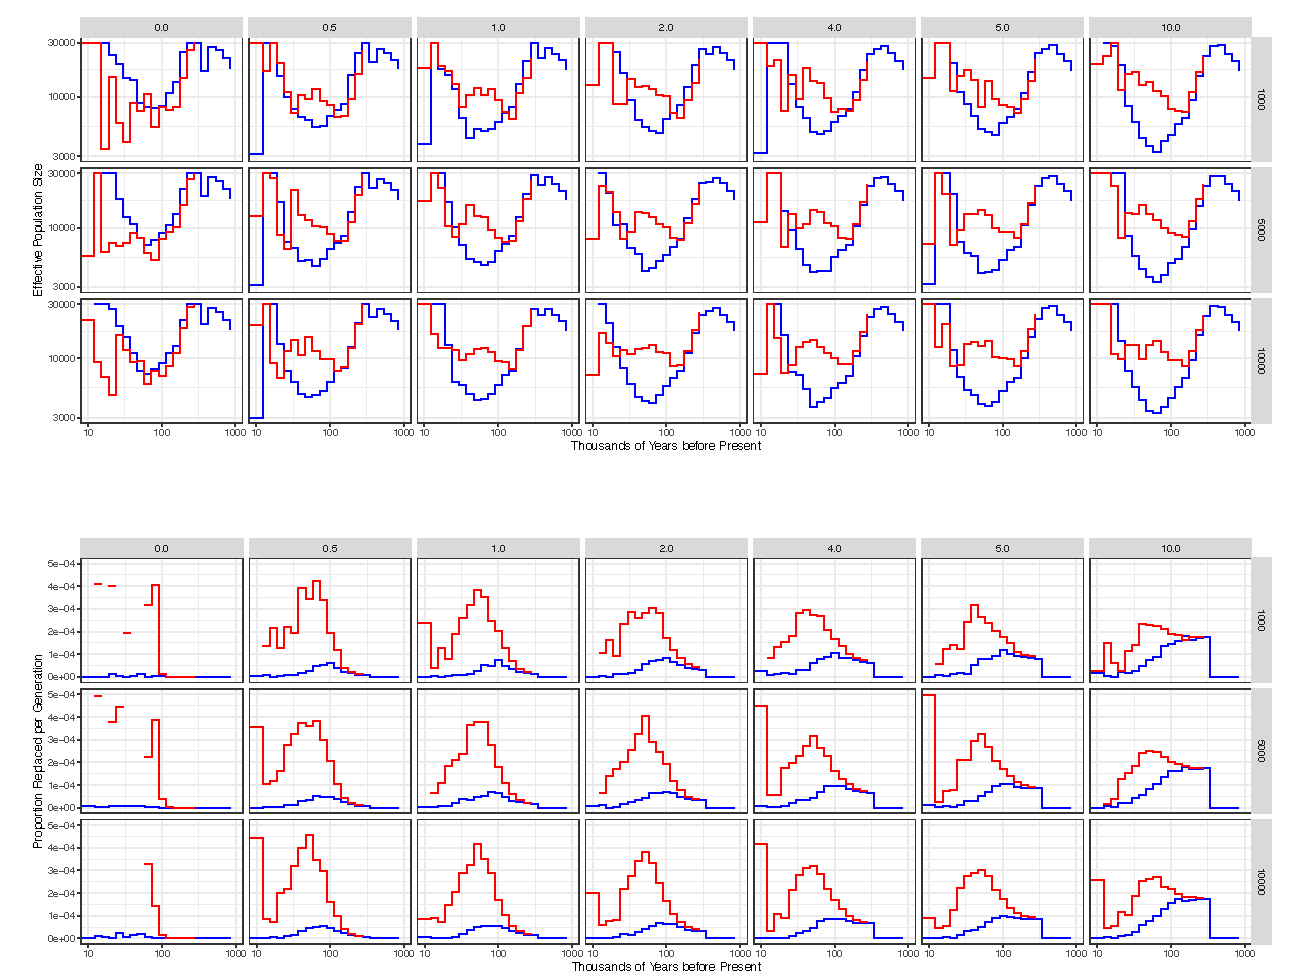
\includegraphics[width=\textwidth]{../plot/mig/yri_dif_migs.pdf}
	\caption{Effective population size and migration history of a Yoruban ({\tt S\_Yoruba-1}) and a French ({\tt S\_French-1}) individual from the Simons Genome Diversity panel. The initial migration proportion was varied along the X axis, while the number of particles is varied along the Y. 10 iterations of variational Bayes was used for parameter inference, while 5000 particles were used to sample from the posterior distribution of trees.}
	\label{init_yri}
\end{figure}

\newpage
\section{Average $D$ Statistics Among Populations}

Here we consider the case of instantaneous admixture explored by Durand et al 2011 when a representative sample from the admixing population is available. Here, the expectation of $D$ is reduced to 
\small 
$$ \begin{aligned} E[  D(P_2, P_1, P0, O)] 
	&= \frac{\text{Pr(ABBA)} - \text{Pr(BABA)}}{\text{Pr(ABBA)} + \text{Pr(BABA)}} \\
&= \frac{3f[t_{P3} - t_{GF}]}{3f [t_{P3} - t_{GF}] + 4N(1-f) (1 - \frac{1}{2N})^{t_{P3}-  t_{P2}} + 4Nf (1 - \frac{1}{2N})^{t_{P3}-t_{GF}}} \end{aligned}$$

where $t_{P_i}$ is the expected time to coalescence of any two lineages in $P_i$, $f$ is the proportion of gene flow while $t_{GF}$ is its timing, and $N$ is the population size. We consider the case where $D$ statistics $D(A_i, A_{pi}, Y, C)$ are summed and divided by their count. In this case, both $A_i$ and $A_{pi}$ are drawn from the same population, which implies that $t_{P_3}$ is constant (with the exception of the San, who are excluded from these calculations). Since we assume that $t_{P_3}$, $f$, $t_{GF}$ are held constant, we straightforwardly rearrange the definition of the $D$ statistic to show that the expectation of averaging over the log of $D$ values for $n$ populations gives the expectation of a $D$ statistic with the average $t_{P2}$, or time to divergence of lineages within the population.  

\resizebox{.75\linewidth}{!}{
	\begin{minipage}{\linewidth}
	$$ \begin{aligned}
	\mathbb{E} [\frac{1}{n} \sum^n_i \ln D(P2, P1, P0, O)] &= \frac{1}{n} \sum^n_i \mathbb{E}[ \ln D(P2, P1, P0, O)] \\
	&= \frac{1}{n} \sum^n_i \ln \frac{3f[t_{P3} - t_{GF}]}{3f [t_{P3} - t_{GF}] + 4N(1-f) (1 - \frac{1}{2N})^{t_{P3}-  t_{P2}} + 4Nf (1 - \frac{1}{2N})^{t_{P3}-t_{GF}}} \\
	&= \frac{1}{n} \sum^n_i \ln \left( 3f[t_{P3} - t_{GF} \right) - \ln ( 3f [t_{P3} - t_{GF}] + 4N(1-f) (1 - \frac{1}{2N})^{t_{P3}-  t_{P2}} \\  &+ 4Nf (1 - \frac{1}{2N})^{t_{P3}-t_{GF}}) \\
	&= \frac{1}{n} \sum^n_i \ln \left( 3f[t_{P3} - t_{GF} \right) - \ln \left( 3f [t_{P3} - t_{GF}] \right) + \ln \left( 4N(1-f) (1 - \frac{1}{2N})^{t_{P3}-  t_{P2}} \right) \\  &- \ln \left( 4Nf (1 - \frac{1}{2N})^{t_{P3}-t_{GF}} \right) \\
	&= \frac{1}{n} \left( n \left( \ln \left( 3f[t_{P3} - t_{GF} \right) + \ln \left( 3f [t_{P3} - t_{GF}] \right) +  + \ln \left( 4Nf (1 - \frac{1}{2N})^{t_{P3}-t_{GF}} \right) \right) \right) \\ &+ \sum^n_i \ln \left( 4N(1-f) (1 - \frac{1}{2N})^{t_{P3}-  t_{P2}} \right) \\
	&= \ldots \sum^n_i (t_{P3}-  t_{P2} ) \ln \left( 4N(1-f) (1 - \frac{1}{2N}) \right) \\
	&= \ldots n \ln \left( 4N(1-f) (1 - \frac{1}{2N}) \right) \sum^n_i (t_{P3}-  t_{P2} ) \\
	&= \ldots n \ln \left( 4N(1-f) (1 - \frac{1}{2N}) \right) \left( \sum^n_i t_{P3} - \sum^n_i t_{P2} \right) \\
	&= \ldots n t_{P3}\ln \left( 4N(1-f) (1 - \frac{1}{2N}) \right) \left(- \sum^n_i t_{P2} \right) \\
	& \text{multiply through the } \frac{1}{n} \ldots \\
	&= \ln \left( 3f[t_{P3} - t_{GF} \right) + \ln \left( 3f [t_{P3} - t_{GF}] \right) +  \ln \left( 4Nf (1 - \frac{1}{2N})^{t_{P3}-t_{GF}} \right) \\ &+ t_{P3} \ln \left( 4N(1-f) (1 - \frac{1}{2N}) \right) \left(- \frac{1}{n} \sum^n_i t_{P2} \right) \\
	&= \ln \left( 3f[t_{P3} - t_{GF} \right) + \ln \left( 3f [t_{P3} - t_{GF}] \right) +  \ln \left( 4Nf (1 - \frac{1}{2N})^{t_{P3}-t_{GF}} \right) \\ &+ \ln \left( 4N(1-f) (1 - \frac{1}{2N})^{t_{P3} - \frac{1}{n} \sum^n_i t_{P2}} \right) \\
	&= \ln \frac{3f[t_{P3} - t_{GF}]}{3f [t_{P3} - t_{GF}] + 4N(1-f) (1 - \frac{1}{2N})^{t_{P3}-  \frac{1}{n} \sum^n_i t_{P2}} + 4Nf (1 - \frac{1}{2N})^{t_{P3}-t_{GF}}} \\
	&= \ln D(\bar{P2}, \bar{P1}, P0, O)
	\end{aligned} $$
\end{minipage}
}

Therefore, the expectation of average $D$ statistics where both $P_1$ and $P_2$ are drawn from the same population produces the expectation of the $D$ statistic with the average within-population coalescent rate. 

\end{document}
